\documentclass{apmcmthesis}
\usepackage{url}
\usepackage{subfigure}
%%%%%%%%%%%%填写相关信息%%%%%%%%%%%%%%%%%%%%%%%%%%
\tihao{B}                            %选题
\baominghao{apmcm2305948}                 %参赛编号
\begin{document}

\pagestyle{frontmatterstyle}

%%%%%%%%%%%%摘要和关键词%%%%%%%%%%%%%%%%%%%%%%%%%%
\begin{abstract}
Crop productivity in greenhouses is influenced by climate factors like temperature, humidity, and wind speed. To address this, a fluid dynamics model using \textbf{Navier-Stokes equations, energy conservation, and Darcy-Forchheimer equations} quantifies airflow and temperature distribution. Simulations are performed with COMSOL software.

In question one, a simplified model uses the \textbf{Reynolds number} under greenhouse conditions, incorporating incompressible laminar flow and heat exchange. Results indicate airflow and temperature changes in different greenhouse areas. \textbf{It is concluded that the wind speed in the middle of the greenhouse can reach 0.2 m/s, and the wind speed on both sides can reach 0.3 m/s. The temperature near the greenhouse fan has risen to 40 degrees Celsius, and the temperature in the further area from the fan has remained around 21-23 degrees}.

In question two, crop growth models are compared, considering crop resistance to fluid flow. The Darcy-Forchheimer equation is added to the previous model. Results show:\textbf{The average air velocity of 0.21 m/s at 0.5 m above the ground was lower than the optimal wind speed of 0.31 m/s, and the plant canopy was not in the optimal wind speed area. The average velocity of the airflow at 0.1 m above the ground is 0.24 m/s, which is also lower than the optimal wind speed}.

In question three, simulations explore two scenarios based on the previous model.  The first involves a vent positioned at 1.3 meters with a ventilation rate of 3 m/s, sustaining favorable conditions despite marginally lower wind speeds. The second scenario, featuring a lower vent at 1 meter and a ventilation rate of 2 m/s, fosters a more conducive environment for plant growth.

In the fourth question, building on the analysis from the previous three questions, we compared and analyzed the impact of factors such as wind speed and fan placement on the design of greenhouse fans in a glass greenhouse. We have proposed a reasonable solution: \textbf{placing the fans at a height of 1m to 1.5m, with a wind speed of 2.5m/s to 3m/s. Additionally, planting heat-loving crops near the fans}. These solutions can provide an optimal growth environment for crops.

Our models provide a comprehensive framework for understanding and optimizing greenhouse environments. They consider both fluid dynamics and plant-crop interactions, offering a holistic approach to greenhouse management. Through simulations, we explored scenarios with different ventilation setups. \textbf{These simulations indicated that altering the position of vents and adjusting ventilation rates can create more conducive environments for plant growth by optimizing temperature and wind speeds.}

In summary, our model demonstrates a propensity to effectively converge with simulation scenarios and holds significant research value for enhancing glass greenhouse systems.
\keywords{Navier-Stokes equations\quad  Energy conservation\quad   Darcy-Forchheimer equations\quad Greenhouse}
\end{abstract}



\newpage
%%%%%%%%%%%%目录%%%%%%%%%%%%%%%%%%%%%%%%%%
\tableofcontents


\newpage
\pagestyle{mainmatterstyle}
\setcounter{page}{1}
%%%%%%%%%%%%问题背景、重述和工作%%%%%%%%%%%%%%%%%%%%%%%%%%
\section{Introduction}
\subsection{Problem Background}
The productivity of crops grown in greenhouses is significantly influenced by a range of climatic factors, such as temperature, humidity, and the speed of the wind.\cite{1}Among these factors, optimal temperature and wind speed are particularly critical for the healthy growth of plants.\cite{2}
%在温室内种植的作物的生产力显著受到多种气候因素的影响,例如温度、湿度和风速。在这些因素中,适宜的温度和风速对植物的健康生长尤为关键。

To regulate climate factors like temperature and wind speed within glass greenhouses, ventilation systems equipped with greenhouse fans are integral to their design, as shown in Figure ~\ref{Image of greenhouse}. The placement of these fans and the rate at which warm air is expelled play a pivotal role in shaping the distribution and evenness of both the velocity and temperature fields inside the greenhouse. Consequently, optimizing the use of greenhouse fans to achieve desirable wind speeds and temperatures, while enhancing their uniformity, represents a crucial challenge in contemporary glass greenhouse design.
%为了调节玻璃温室内的气候因素,如温度和风速,通常在温室设计中使用配备有温室风扇的通风系统,如图1所示。温室风扇的位置以及温暖空气排出的速度对温室内速度场和温度场的分布和均匀性有着决定性的影响。因此,如何优化温室风扇以获得合适的风速和温度,并提高它们的均匀性,是当前玻璃温室设计中需要解决的一个重要问题。

\begin{figure}[htbp]
  \centering
  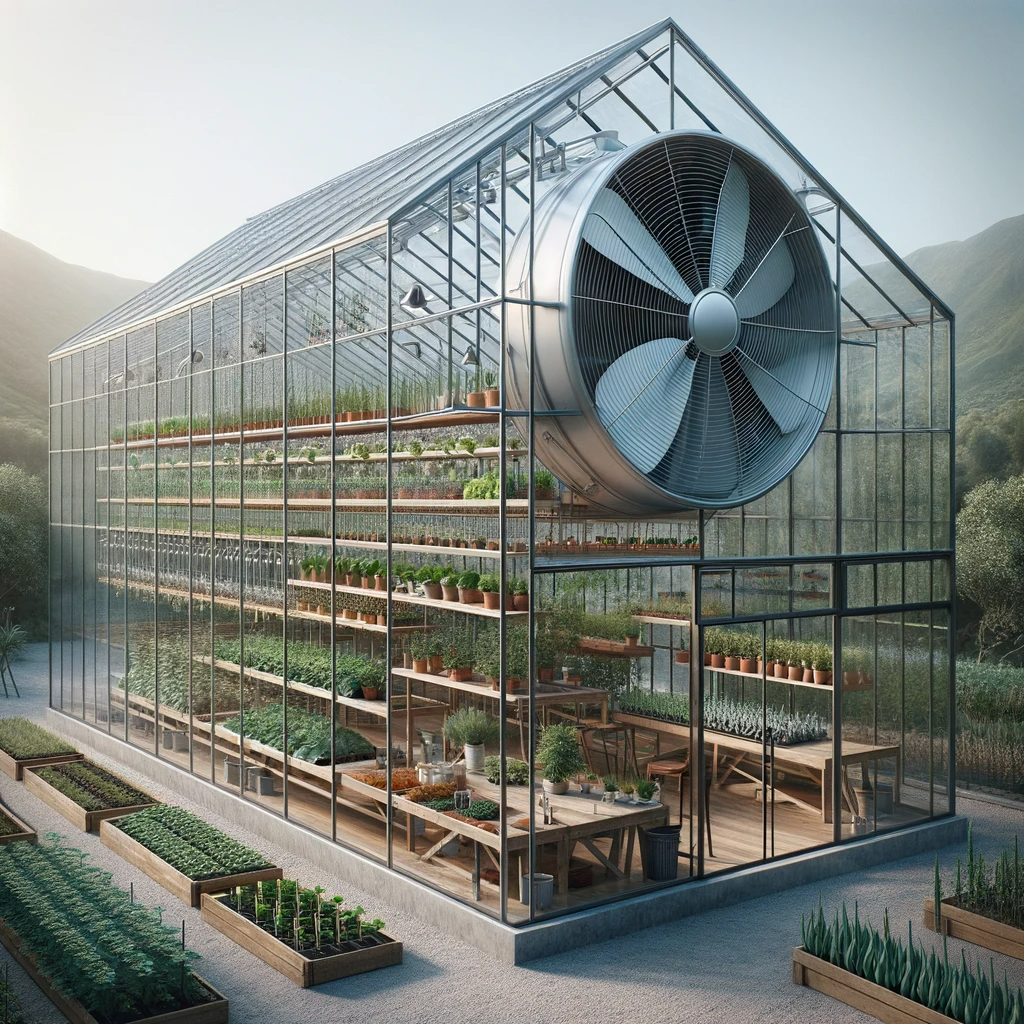
\includegraphics[width=10cm,height=6cm]{figures/GreenHouse.png}
  \caption{Image of greenhouse}
  \label{Image of greenhouse}
\end{figure}

\subsection{Restatement of the Problem}
\subsubsection{Data of the Problem}
\begin{itemize}
  \item \textbf{Glass Greenhouse Design}
  
  (1)The glass greenhouse has dimensions of 10 meters by 3 meters by 2 meters, with a 0.5-meter by 0.5-meter greenhouse fan inside.
  
  (2)The greenhouse fan operates with velocity inlet conditions, blowing warm air at 40 degrees Celsius at an average velocity of 2 meters per second.
  
  (3)The outer glass and bottom soil of the greenhouse are set as wall conditions, exchanging energy with the entire greenhouse through convective heat transfer and conduction.\cite{3}
%玻璃温室设计:(1)玻璃温室尺寸为10米×3米×2米,内部有一个0.5米×0.5米的温室风扇。(2)温室风扇以速度入口条件运行,吹送温度为40摄氏度的温暖空气,速度为2米/秒。(3)温室的外玻璃和底部土壤被设置为墙壁条件,与整个温室通过对流传热和传导交换能量。
  \item \textbf{Greenhouse Environmental Conditions}

  (1)The initial temperature is set at 20 degrees Celsius.
  
  (2)When planting crops inside the greenhouse, it is necessary to consider the canopy resistance of the crops.
  
  (3)The crop model is simplified as a porous medium with dimensions of 8 meters by 2 meters by 0.5 meters.\cite{4}
%温室环境条件:(1)初始温度设定为20摄氏度。(2)在温室内种植作物时,需要考虑作物的冠层阻力。(3)作物模型被简化为一个尺寸为8米×2米×0.5米的多孔介质。
  \item \textbf{Crop Growth Conditions}

  (1)The suitable wind speed for crop growth inside the greenhouse ranges from 0.3 to 1 meter per second.
  
  (2)The suitable temperature range is between 23 and 26 degrees Celsius.
%作物生长条件:(1)温室内适宜作物生长的风速范围为0.3-1米/秒。(2)适宜的温度范围为23-26摄氏度。
\end{itemize}

\begin{figure}[htbp]
  \centering
  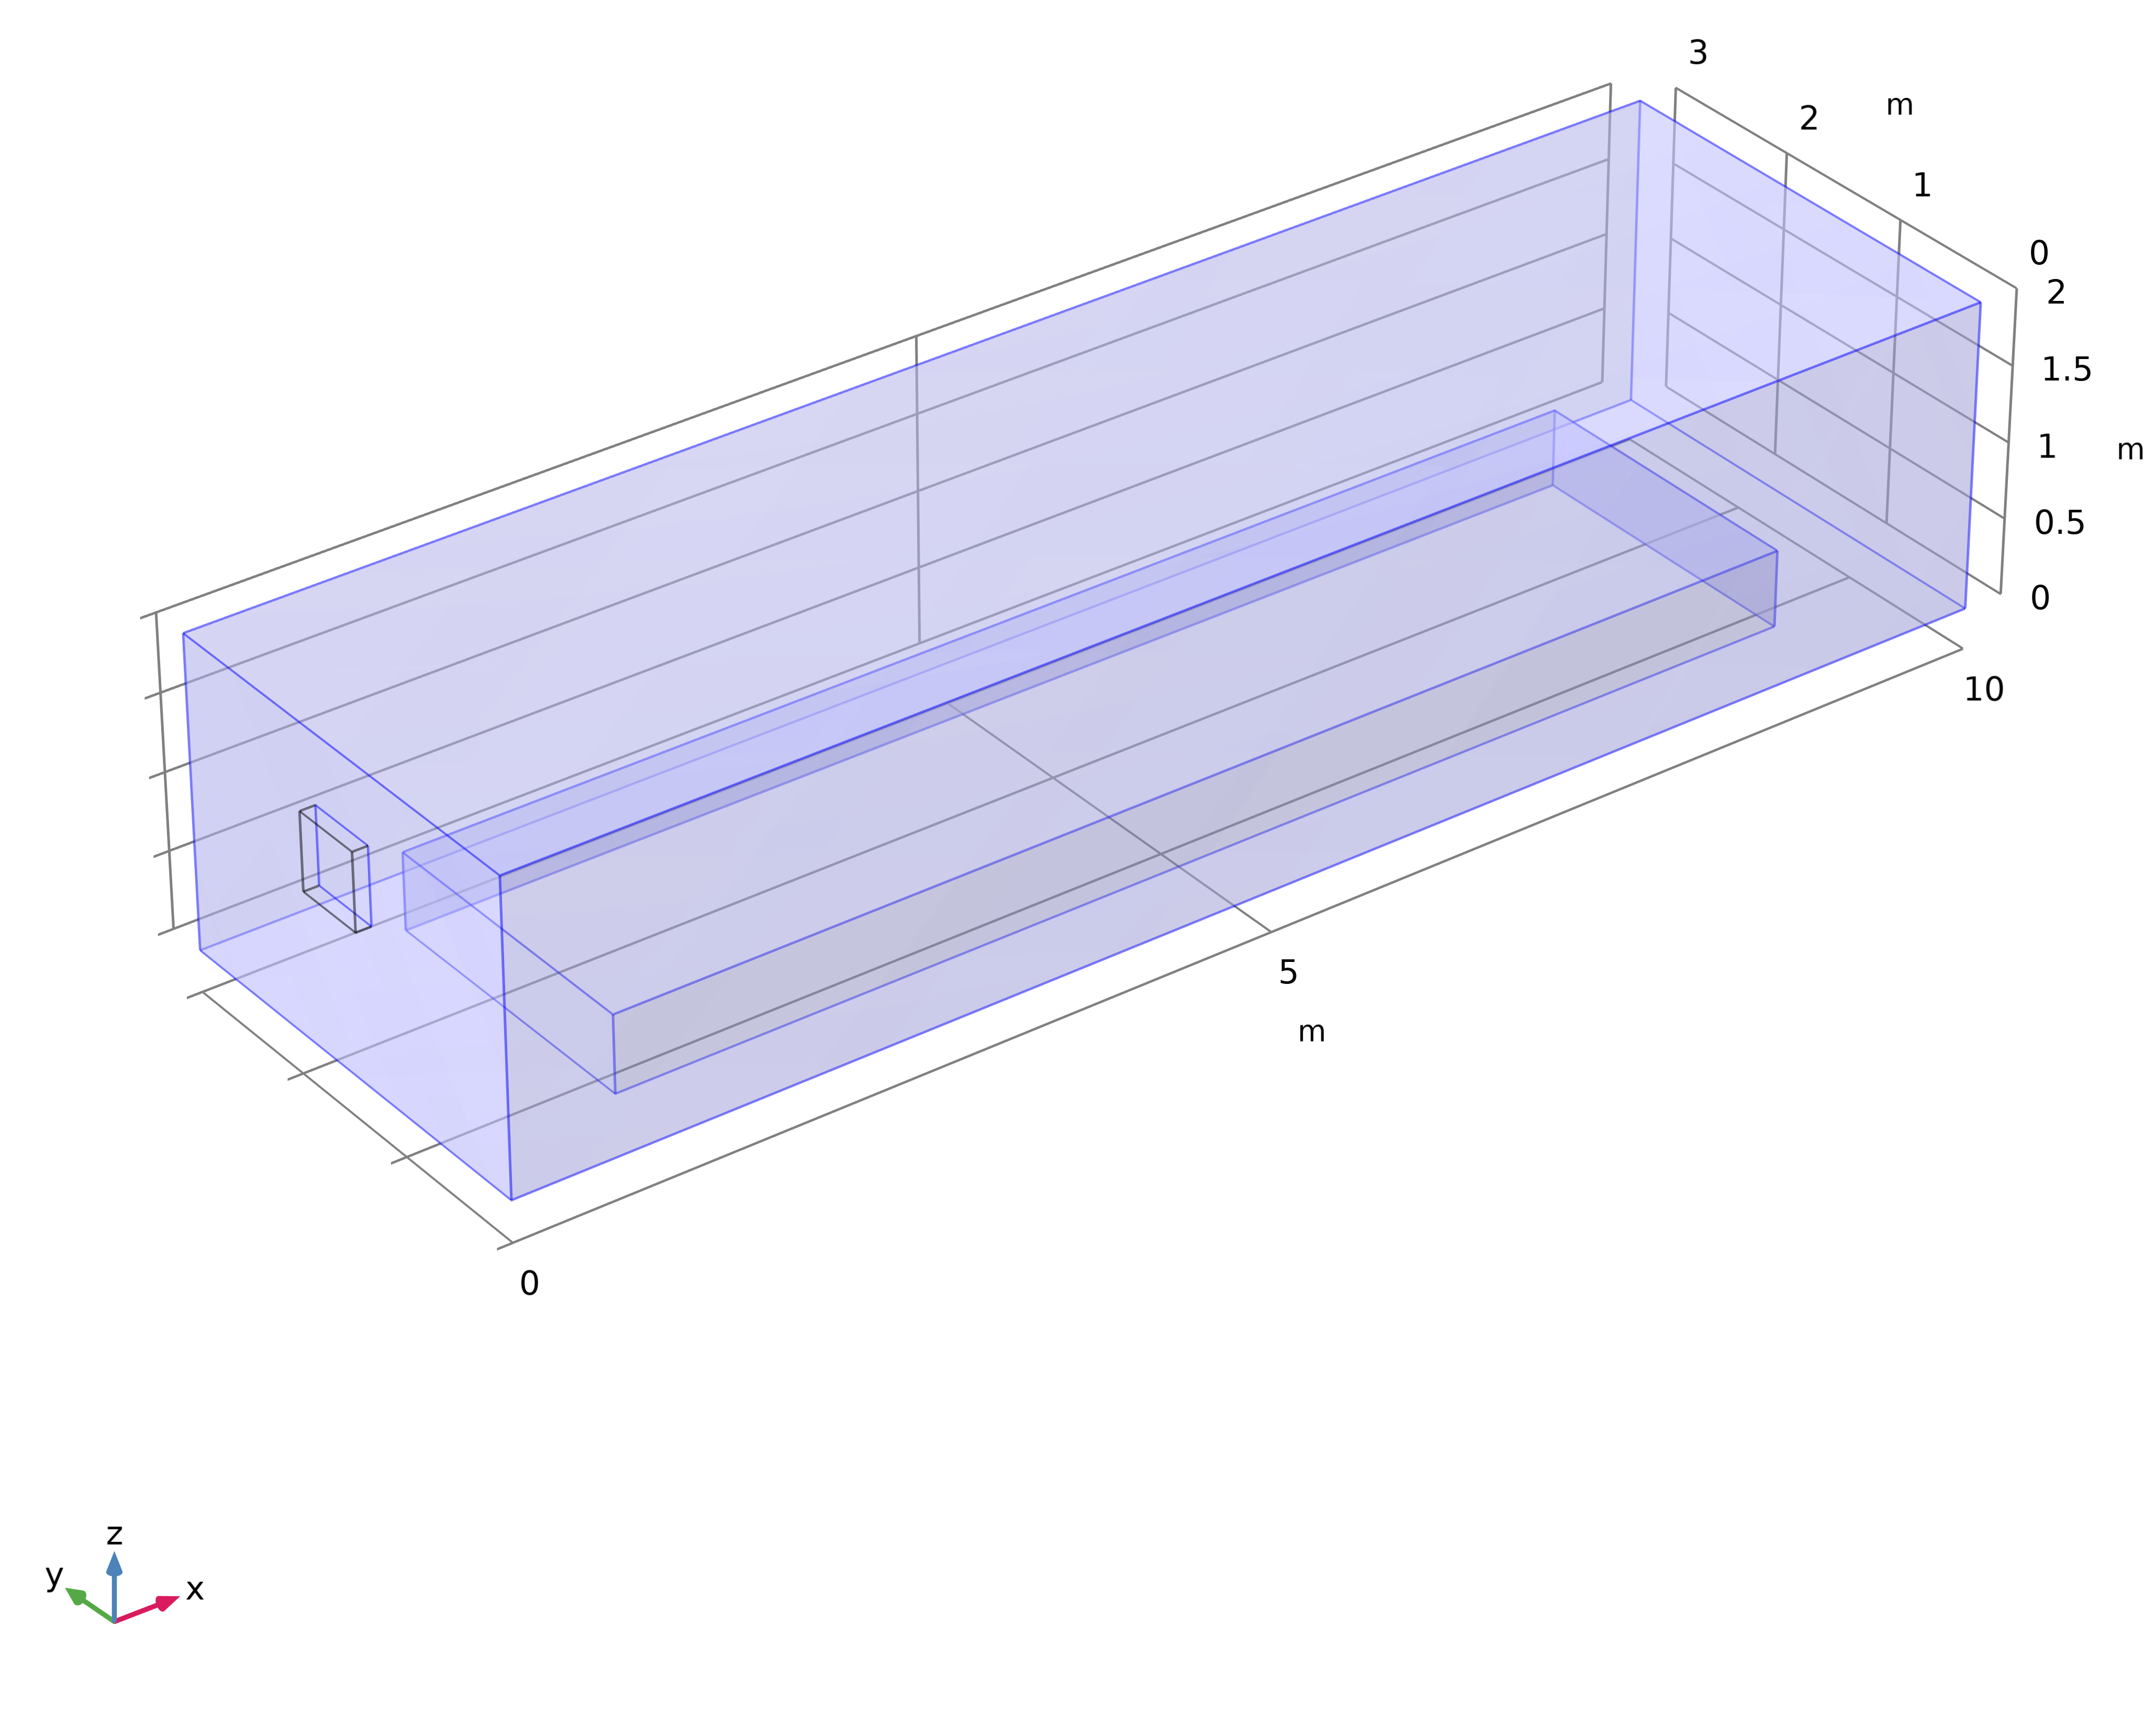
\includegraphics[width=10cm,height=8cm]{figures/Geometric model diagram.png}
  \caption{Geometric model diagram}
  \label{Geometric model diagram}
\end{figure}

\subsubsection{Analysis of Problem}
\begin{itemize}
  \item \textbf{Question 1}
  
  Create a mathematical model to describe the temperature and wind speed distribution within an empty glass greenhouse. Visualize this distribution at a height of 0.5 meters in a cross-section of the greenhouse.
%建立一个数学模型,描述无作物的玻璃温室内温度和风速的分布。在温室的高度为0.5米处,展示温度和风速的分布情况。
  \item \textbf{Question 2}

  Create a mathematical model for temperature and wind speed distribution inside a glass greenhouse with cultivated crops. Show the wind speed and temperature distribution at two cross-sections within the greenhouse: one at 0.5 meters (crop canopy level) and another at 0.1 meters (inside the crop canopy). Assess whether the conditions are conducive to crop growth.
%建立一个关于玻璃温室内种植作物的温度和风速分布的数学模型。展示温室内两个横截面的风速和温度分布:一个位于0.5米高度(作物冠层水平),另一个位于0.1米高度(作物冠层内部)。评估条件是否有利于作物生长。
  \item \textbf{Question 3}

  Provide temperature and wind speed inside the greenhouse for two scenarios and compare them with the solution in the second question. In Scenario One, increase warm air outlet speed from 2 m/s to 3 m/s. In Scenario Two, lower the greenhouse fan position from 1.3 m to 1 m.
%提供玻璃温室内以下两种情况的温度和风速分布,并与第二个问题中的解决方案进行比较。在第一种情况下,将温暖空气出口速度从2 m/s增加到3 m/s。在第二种情况下,通过将温室风扇位置从1.3 m降低到1 m。
  \item \textbf{Question 4}

  Optimize the glass greenhouse fan design by considering factors like fan quantity, placement, wind speed, temperature, specifications, and crop variations.
%考虑因素如风扇数量、位置、风速、温度、规格和不同作物,进一步优化玻璃温室风扇设计。
\end{itemize}

\subsection{Our Work}
\begin{itemize}
  \item \textbf{Question 1}

  By solving the Reynolds number of the greenhouse space conditions, the model is further simplified, and the incompressible laminar flow model is used, and then coupled with the temperature field of convective heat transfer and conduction exchange energy, the airflow and temperature changes caused by warm air are simulated, and then the COMSOL software is used to simulate and solve. Finally, it is concluded that the wind speed in the middle of the greenhouse can reach 0.2 m/s, and the wind speed on both sides can reach 0.3 m/s. The temperature near the greenhouse fan has risen to 40 degrees Celsius, and the temperature in the further area from the fan has remained around 21-23 degrees
  \item \textbf{Question 2}
  
   By reviewing the literature and comparing the fitting results of different models to crops, the motion of crops to the fluid was considered, and the resistance generated by the main generation slowed down the movement of the fluid. We use the Darcy-Forchheimer equation to further constrain the model of problem one. The average air velocity of 0.21 m/s at 0.5 m above the ground was lower than the optimal wind speed of 0.31 m/s, and the plant canopy was not in the optimal wind speed area. The average velocity of the airflow at 0.1 m above the ground is 0.24 m/s, which is also lower than the optimal wind speed, all in all, the temperature is suitable under this condition, and the wind speed is slow, which is not very suitable for plant growth.
  \item \textbf{Question 3}

  On the model of the second question, a simulation is carried out. (1) The simulation results of the vent located at 1.3m and the ventilation 3m/s are as follows: the velocity of the vent increases from 2m/s to 3m/s, the temperature does not change greatly, most areas are suitable for plant growth, the average air velocity of 0.2m/s at 0.5 m from the ground is lower than the optimal wind speed of 0.31m/s, the average flow velocity of the airflow at 0.1 m from the ground is 0.32m/s, which is close to the optimal wind speed, and the internal wind speed of the crop canopy is suitable. The wind speed is faster than the air outlet speed of 2m/s, but it is still slow, compared to the original scene, this scene is still very suitable for plant growth. (2) The simulation results of the vent located at 1m and the ventilation of 2m/s: the height of the air outlet drops from 1.3m to 1m, the average temperature is 25 degrees, which is warmer than the other two scenarios, the average air velocity at 0.5 m from the ground is close to the optimal wind speed, which is larger than the wind speed in the original scene and scenario 1, the wind speed in the crop canopy is appropriate, the average air velocity at 0.1 m from the ground is 0.33m/s close to the optimal wind speed, and the internal wind speed of the crop canopy is appropriate. All in all, the temperature and wind speed are suitable under this condition, which is more suitable for plant growth than scenario 1 and the original scenario.
 
  \item \textbf{Question 4}

  For question 4, on the basis of the first three questions, we compare and analyze the influence of the wind speed and position of the fan on the flow rate and temperature of different greenhouse sections, which can infer the internal law of the device, and give better suggestions: reasonable placement of the fan position, blowing temperature, the number of fans, etc
\end{itemize}

%%%%%%%%%%%%模型假设%%%%%%%%%%%%%%%%%%%%%%%%%%
\section{Model Assumptions}
\begin{itemize}
\item 
The fan blows out without turbulence and the direction of velocity points to the y-axis.
\item
The density of the fluid is uniform and does not change over time.
\item
Due to the relatively slow flow rate of the fluid, it is considered an incompressible fluid and flows as laminar.
\item 
The air quality is light, and gravity has a negligible effect on gas flow.
\item
The walls are smooth and immovable.
\item
The air viscosity is small and flows at a low velocity, which produces less stress and ignores stress heat generation.
\item
The heat flux on the wall is zero.
\item
The effects of plant respiration, photosynthesis, etc. on indoor temperature and wind speed are not considered.
\item
Not considered greenhouse doors, drafts, solar radiation, and other environmental factors.
\end{itemize}

%%%%%%%%%%%%符号说明%%%%%%%%%%%%%%%%%%%%%%%%%%
\section{Symbol Description}
\begin{table}[htbp]
  \centering
  \label{Symbol Description}
  \caption{Symbol Description}
  \begin{tabular}{ccccccc}
   \toprule
    Symbols & ~~~~~~~~~ & Meaning & ~~~~~~~~~ & Unit \\
   \midrule
   $\rho$ & ~~~~~~~~~ & Density & ~~~~~~~~~ & m/s \\
   $t$   & ~~~~~~~~~ & Time  & ~~~~~~~~~ & s \\
   $u,v,w$   & ~~~~~~~~~ & The velocity is a component of the lower x, y, z axis & ~~~~~~~~~ & m/s \\
   $\textbf{u}$   & ~~~~~~~~~ & Velocity vectors & ~~~~~~~~~ & m/s \\
   $i$    & ~~~~~~~~~ & Internal energy & ~~~~~~~~~ & J \\
   $q_x,q_y,q_z$    & ~~~~~~~~~ & The component of the heat flux in all directions & ~~~~~~~~~  & $w/m^2$ \\
   $c_v$   & ~~~~~~~~~ & Must have a heat capacity  & ~~~~~~~~~ & J/(Kg·k)\\
   $k$   & ~~~~~~~~~  & Permeability coefficient  & ~~~~~~~~~ & m/s \\
   $q$   & ~~~~~~~~~  & Flow rate of the fluid  & ~~~~~~~~~ &  $ m^3/s $\\
   $A$   & ~~~~~~~~~  & Cross-sectional area  & ~~~~~~~~~ & $ m^2 $ \\
   $\bigtriangleup h$    & ~~~~~~~~~ & Hydraulic head difference & ~~~~~~~~~  & m \\
   $L$   & ~~~~~~~~~  & Length of the flow path & ~~~~~~~~~ & $ m $ \\
   $p$   & ~~~~~~~~~  & Pressure & ~~~~~~~~~ &  $p_a$ \\
   $S_\varphi$   & ~~~~~~~~~ & Momentum source term  & ~~~~~~~~~ &  $ Kg\cdot m/s $ \\
   $K_p$   & ~~~~~~~~~& Permeability coefficient of the porous medium & ~~~~~~~~~ &   m/s \\
    $\mu$   & ~~~~~~~~~ & Dynamic viscosity of air & ~~~~~~~~~ &  $ p_a \cdot s $ \\
   
   \bottomrule
\end{tabular}
\end{table}

\begin{table}[]
    \centering
    \caption{Symbol Description}
    \begin{tabular}{ccccccc}
     \toprule
    Symbols & ~~~~~~~~~\qquad \qquad & Meaning & \qquad \qquad ~~~~~~~~~ & Unit \\
   \midrule
   $C_F$   &  ~~~~~~~~~ & Nonlinear momentum loss coefficient & ~~~~~~~~~ &  none \\
   $I_LAP$   &  ~~~~~~~~~ & Leaf area index  & ~~~~~~~~~ &  $ cm^2/g $ \\
   $ C_D $   & ~~~~~~~~~  & Drag coefficient of the crop canopy & ~~~~~~~~~ &  none\\
   \bottomrule
    \end{tabular}
    
    \label{tab:my_label}
\end{table}

%%%%%%%%%%%%模型的建立和求解%%%%%%%%%%%%%%%%%%%%%%%%%%
\section{Models}
\subsection{Physical basis of the model}
%最基本的物理学公式
\subsubsection{Principle of Continuity}
%连续性方程
The first step in deriving the mass conservation equation is to establish the mass balance of a fluid element: the rate of change of mass within the fluid element is equal to the net mass flow rate into the fluid element.\cite{5}
%推导质量守恒方程的第一步是建立流体元的质量平衡:流体元内质量的变化率等于流入该流体元的净质量流量。

The rate of increase of mass within a fluid element is:
%流体元内质量的增加率是

\begin{equation}
\frac{\partial }{\partial t} (\rho \delta x \delta y \delta z) = \frac{\partial \rho}{\partial t} (\delta x \delta y \delta z) 
\end{equation}

Next, we will describe the mass flow rate entering the fluid element through the boundary interface, which is determined by the product of density, area, and the component of the normal velocity on the interface. As shown in Figure ~\ref{Mass flow through a fluid element}, the mass flow rate entering the fluid element through the boundary interface is:
%接下来,我们将描述通过边界界面净流入流体元内的质量流量,这是由密度、面积以及界面上法向速度分量的乘积来确定的。从图中可以看出,通过边界界面净流入流体元内的质量流量是

\begin{equation}
\begin{aligned}
&(\rho u-\frac{\partial (\rho u)}{\partial x}\frac{\delta x}{2}  )\delta y\delta z-(\rho u+\frac{\partial (\rho u)}{\partial x}\frac{\delta x}{2}  )\delta y\delta z\\
+&(\rho v-\frac{\partial (\rho v)}{\partial y}\frac{\delta y}{2}  )\delta x\delta z-(\rho v+\frac{\partial (\rho v)}{\partial y}\frac{\delta y}{2}  )\delta x\delta z\\
+&(\rho w-\frac{\partial (\rho w)}{\partial z}\frac{\delta z}{2}  )\delta x\delta y-(\rho w+\frac{\partial (\rho w)}{\partial z}\frac{\delta z}{2}  )\delta x\delta y
\end{aligned}
\end{equation}

All terms of the mass balance equation are placed on the left side of the equation, and the expression is divided by the volume of the fluid element, denoted as $\delta x\delta y\delta z$.
%质量平衡式的所有项放到等号左边,用流体元的体积δxδyδz除表达式得到

\begin{equation}
\begin{aligned}
&\frac{\partial \rho }{\partial t}+\frac{\partial (\rho u)}{\partial x}+\frac{\partial (\rho v)}{\partial y}+\frac{\partial (\rho w)}{\partial z}=0\\
&\frac{\partial \rho }{\partial t}+\nabla\cdot (\rho \textbf{u})=0
\end{aligned}
\end{equation}

\begin{figure}[htbp]
  \centering
  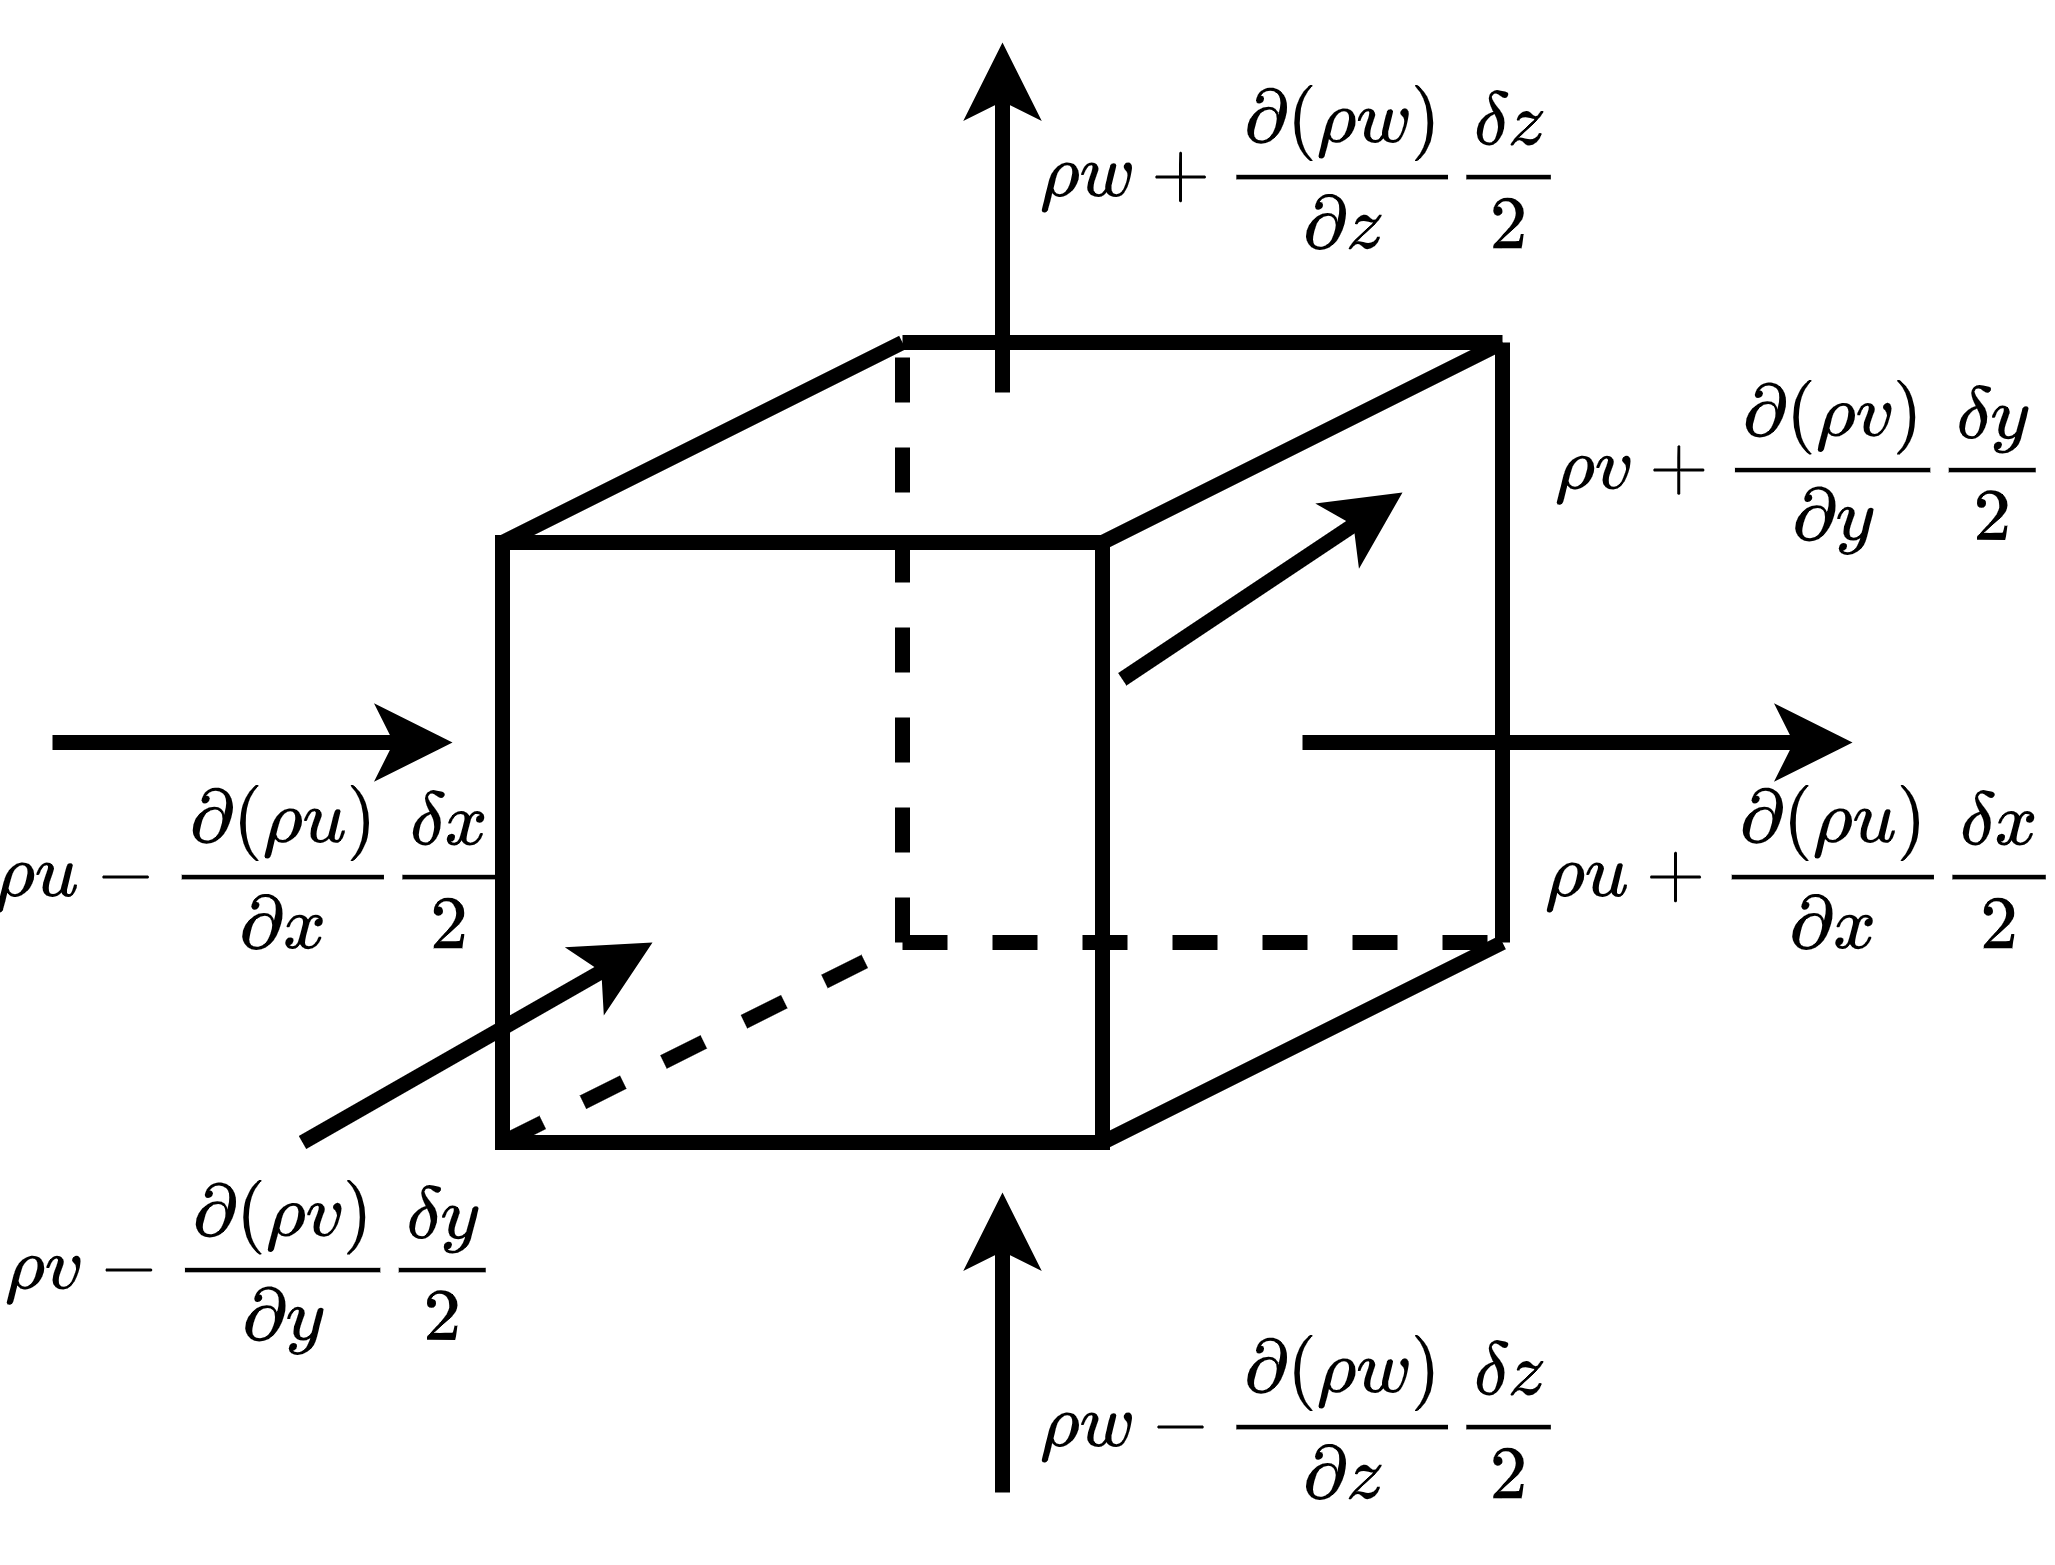
\includegraphics[width=10cm,height=7cm]{figures/Mass flow through a fluid element.png}
  \caption{Mass flow through a fluid element}
  \label{Mass flow through a fluid element}
\end{figure}

In the second term of formula (3), \textbf{u}=(u,v,w), represents the velocity vector, and $\nabla\cdot ()$ denotes the divergence operation on the variables inside the parentheses. It is the unsteady, three-dimensional mass conservation equation or continuity equation for a compressible fluid at a point. The first term on the left-hand side is the rate of change of density (mass per unit volume) with respect to time. The second term describes the net outflow of mass across the boundary.
%公式(3)中第二个,u=(u,v,w)是速度矢,▽·()表示对括号中的变量进行散度运算。其是可压缩流体中一点的非定常、三维质量守恒方程或连续性方程。左边第一项是密度(单位体积的质量)的时间变化率。第二项描述越过边界净流出流。

\subsubsection{Momentum Equation}
%动量方程

Each physical quantity of a fluid particle is a function of the particle's position (x,y,z) and time t, so that the value of this physical quantity per unit mass of fluid is, and the full derivative of the time following the fluid particle can be written as
%流粒子的每一个物理量是粒子的位置(x,y,z)和时间t的函数,令每单位质量流体的这个物理量的值为,跟随流体粒子的时间全导数可写为
\begin{equation}
\frac{\mathrm{d} \varphi }{\mathrm{d} t} =\frac{\partial \varphi }{\partial t} +\frac{\partial \varphi }{\partial x}\frac{\mathrm{d} x}{\mathrm{d} t}+ \frac{\partial \varphi }{\partial y}\frac{\mathrm{d} y}{\mathrm{d} t}+\frac{\partial \varphi }{\partial z}\frac{\mathrm{d} z}{\mathrm{d} t} 
\end{equation}

The fluid particles move with the fluid, so dx/dt=u, dy/dt=v, dz/dt=w, and then the derivative of matter for $\varphi$ is 
%流体粒子随流体运动,因此dx/dt=u,dy/dt=v,dz/dt=w,于是\varphi的物质导数为
\begin{equation}
\frac{\mathrm{d} \varphi }{\mathrm{d} t} =\frac{\partial \varphi }{\partial t} +u\frac{\mathrm{d} x}{\mathrm{d} t}+ v\frac{\mathrm{d} y}{\mathrm{d} t}+w\frac{\mathrm{d} z}{\mathrm{d} t}+\textbf{u}\cdot \nabla\varphi 
\end{equation}

The rate of change of the fluid particles per unit volume $\varphi$ is given by the product of d$\varphi$/dt and density $\rho$, so there is
%流体粒子每单位体积\varphi 的变化率由d\varphi/dt和密度\rho 的积给出,于是有
\begin{equation}
\rho \frac{\mathrm{d} \varphi }{\mathrm{d} t} =\rho(\frac{\partial \varphi }{\partial t} +\textbf{u} \cdot \nabla\varphi  )
\end{equation}

The sum of the density change and convection terms of the fluid element in the equation of conservation of mass is
%质量守恒方程中流体元的密度变化和对流项之和是
\begin{equation}
\frac{\partial \rho }{\partial t} +\nabla\cdot (\rho \textbf{u} )
\end{equation}

Generalized to any conserved quantity $\varphi$
%推广到任意守恒量\varphi ,可得
\begin{equation}
\frac{\partial \rho \varphi }{\partial t} +\nabla\cdot (\rho \varphi \textbf{u} )
\end{equation}

Rewrite it in relation to the material derivative of $\varphi$ on the basis of the above equation
%在上式基础上重写它与\varphi的物质导数的关系
\begin{equation}
\frac{\partial (\rho \varphi )}{\partial t} +\nabla\cdot (\rho \varphi \textbf{u})=\rho [\frac{\partial \varphi }{\partial t}+ \textbf{u}\cdot \nabla\varphi]+\varphi[\frac{\partial \rho }{\partial t}+\nabla\cdot(\rho \textbf{u}) ]=\rho \frac{\mathrm{d} \varphi }{\mathrm{d} t} 
\end{equation}

To construct the three components of the momentum equation, u, v, and w are used instead of $\varphi$ in the above formula
%为构造动量方程的三个分量式,分别用u、v和w代替上述公式里面的\varphi,得
\begin{equation}
\begin{aligned}
&\rho \frac{\mathrm{d} u}{\mathrm{d} t}=\frac{\partial (\rho u)}{\partial t}+\nabla\cdot (\rho u\textbf{u})  \\
&\rho \frac{\mathrm{d} v}{\mathrm{d} t}=\frac{\partial (\rho v)}{\partial t}+\nabla\cdot (\rho v\textbf{u})\\
&\rho \frac{\mathrm{d} w}{\mathrm{d} t}=\frac{\partial (\rho w)}{\partial t}+\nabla\cdot (\rho w\textbf{u})
\end{aligned}
\end{equation}

Viscous stress is denoted as $\tau$, and the resultant force acting on the fluid by surface stress per unit volume is equal to the sum of the net forces on the three opposite surfaces divided by volume, considering the force acting in the x-direction. At the same time, the x-component of the momentum equation can be obtained by using the source term of the momentum per unit time and per unit volume in the x-direction $S_{Mx}$, and the same can be said for the y and z directions.
%粘性应力记为\tau ,考虑x方向作用的力,通过表面应力作用在流体上单位体积的合力等于三对面上的净力之和除以体积。同时,可以用单位时间、单位体积x方向动量的源项S_{Mx}得到动量方程的x分量式,同理可以推出y和z方向的。
\begin{equation}
\begin{aligned}
&\rho \frac{\mathrm{d} u}{\mathrm{d} t} =\frac{\partial (-p+\tau _{xx}) }{\partial x} +\frac{\partial \tau _{yx}}{\partial y}+\frac{\partial \tau _{zx}}{\partial z}+S_{Mx}\\
&\rho \frac{\mathrm{d} v}{\mathrm{d} t} =\frac{\partial (-p+\tau _{yy}) }{\partial y} +\frac{\partial \tau _{xy}}{\partial x}+\frac{\partial \tau _{zy}}{\partial z}+S_{My}\\
&\rho \frac{\mathrm{d} w}{\mathrm{d} t} =\frac{\partial (-p+\tau _{zz}) }{\partial z} +\frac{\partial \tau _{xz}}{\partial x}+\frac{\partial \tau _{yz}}{\partial y}+S_{Mz}\\
\end{aligned}
\end{equation}

\subsubsection{Energy Equation}
%能量方程

The rate of energy increase of the fluid particle is equal to the sum of the heating rate given to the fluid particle and the power to the fluid particle. The increase rate of energy per unit volume is:
%流体粒子的能量增加率等于给流体粒子的加热率与对流体粒子的功率之和。单位体积能量增加率为:
$$\rho \frac{\mathrm{d} i}{\mathrm{d} t} $$

$i$ is the internal energy, that is, the energy per unit mass of fluid. Here, since the airflow is not very fast, ignore the effect of the stress generated by the viscosity and increase the internal energy of the control element. Considering only the change in internal energy caused by heat conduction, if the heat flux vector $Q$ has three components, $q_x, q_y, q_z$. The net heat transfer rate in the x-direction is the difference between the heat input rate of the crossing surface $W$ and the heat loss rate of the crossing surface $E$:
%$i$为内能,即单位质量流体能量。在这里由于空气流动并不是很快,忽略黏度产生应力而使控制元内能增加的影响。仅考虑热传导带来的内能变化,若热通量矢量$Q$的有三个分量$q_x,q_y,q_z$。在x方向上的净传热率为越过面$W$的热输入率和越过面$E$的热损失率之差:
$$[(q_x-\frac{\partial q_x}{\partial x}\frac{\delta x}{2})-(q_x+\frac{\partial q_x}{\partial x}\frac{\delta x}{2})-(q_x+\frac{\partial q_x}{\partial x}\frac{\delta x}{2})]\delta y\delta z=-\frac{\partial q_x}{\partial x}\delta x\delta y\delta z$$
There is the same equation in the y,z direction. The sum of the above three items is divided by the volume $$\delta x \delta y\delta z$$ to obtain the total heating rate per unit volume of fluid particles:
%在y,z方向上有同样的方程。由以上三项之和同时除以体积$\delta x \delta y\delta z$得到单位体积流体粒子的总加热率:
$$-\frac{\partial q_x}{\partial x} -\frac{\partial q_y}{\partial y}-\frac{\partial q_z}{\partial z}=-\bigtriangledown \cdot q$$
The Fourier theorem is used in the x-direction to relate heat flux and temperature:
%在x方向上利用Fourier定理将热通量和温度联系起来:
$$q_x=-k \frac{\partial q_x}{\partial x}$$
The same is true in the y,z direction. The divergence is calculated on both sides of the equation at the same time to establish the relationship between the heat source and the temperature:
%在y,z方向上同理。对式子两边同时求进行散度运算,建立起热源和温度的关系。
$$-\bigtriangledown  \cdot q=\bigtriangledown \cdot (k\bigtriangledown T)$$
For an incompressible fluid, $i=c_v T$, $c_v$ is the definite heat capacity, $\bigtriangledown \cdot u=0$.
%对于不可压缩的流体而言,$i=c_v T$,$c_v$是必定热容,$\bigtriangledown \cdot u=0$.上式成为温度方程:
$$\rho c_v\frac{\mathrm{d} T}{\mathrm{d} t} =k\bigtriangledown^2T+q$$
where q is the heat source intensity of the external heating source term.
%式子中的q为外加热源项的热源强度。

\subsubsection{Darcy-Forchheimer Equation}
%达西-福尔什海默方程

The Darcy-Forchheimer equation is a fundamental equation used to describe fluid flow in porous media. It finds widespread applications in fields such as groundwater flow, petroleum engineering, soil mechanics, and more。
%达西-福尔什海默方程是描述多孔介质中流体流动的基本方程之一。它在地下水流动、石油工程、土壤力学等领域中有广泛的应用。

The Darcy-Forchheimer equation is typically expressed as:
%达西-福尔什海默方程通常表示为:

\begin{equation}
q = -k \cdot A \cdot \frac{\Delta h}{L}
\end{equation}

Where:
%其中:
\begin{align*}
q & : Flow rate of the fluid \\
k & : Permeability of the porous media \\
A & : Cross-sectional area \\
\Delta h & : Hydraulic head difference \\
L & : Length of the flow path
\end{align*}

This equation describes the relationship between the flow rate of a fluid in porous media and the permeability, cross-sectional area, hydraulic head difference, and length of the flow path.
%这个方程描述了流体在多孔介质中的流动速率与渗透率、横截面积、水头差和流动路径长度之间的关系。

\subsection{Temperature and wind speed distribution in a no-crop glass greenhouse}
%无作物玻璃温室温度和风速分布

\subsubsection{Laminar flow}
% 层流

  Laminar flow is an orderly state of fluid motion, and its theoretical foundation can be described through the mathematical equations of fluid dynamics. Under the condition of incompressible fluid, the primary equations used to express laminar flow are the mass conservation equation and the Navier-Stokes equation. The mass conservation equation states that the fluid density does not change over time, and mass conservation is a critical condition in fluid motion. The mathematical expression is:
  $\nabla \cdot \mathbf{v} = 0$
% 层流是一种流体运动的有序状态,其理论基础可以通过流体动力学的数学方程来描述。在不可压缩流体条件下,主要采用质量守恒方程和Navier-Stokes方程来表达层流的运动。质量守恒方程表示流体的密度不随时间变化,在流体运动中质量守恒是一个关键条件。数学表达式为:

Where $\nabla \cdot \mathbf{v}$ represents the divergence of the fluid velocity field, and when it equals zero, it indicates that mass conservation holds.
% 其中,∇⋅v 表示流体速度场的散度,等于零表示质量守恒成立。

On the other hand, the Navier-Stokes equations describe the motion of fluid under external forces, including acceleration, pressure, and viscous effects. For incompressible fluids, the Navier-Stokes equations can be simplified to:
% 另一方面,Navier-Stokes方程则描述了流体在外力作用下的运动,包括加速度、压力和黏性效应。对于不可压缩流体,Navier-Stokes方程可以简化为:

\begin{equation}
\rho \left(\frac{\partial \mathbf{v}}{\partial t} + \mathbf{v} \cdot \nabla \mathbf{v}\right) = -\nabla p + \mu \nabla^2 \mathbf{v}
\end{equation}

Where \(\rho\) is the fluid density, \(\mathbf{v}\) is the velocity field, \(t\) is time, \(p\) is pressure, and \(\mu\) is the dynamic viscosity coefficient of the fluid.
%其中,ρ 是流体密度,v 是速度场,t 是时间,p 是压力,μ 是流体的动力黏性系数。

In laminar flow conditions, stable streamlines form within the fluid, with minimal velocity differences between adjacent streamlines. This typically occurs at low Reynolds numbers, where the inertial forces are relatively small compared to viscous forces. The occurrence of laminar flow is also influenced by boundary conditions.
% 在层流条件下,流体内部形成了稳定的流线,相邻流线之间的速度差异较小。这通常发生在低雷诺数的情况下,即惯性力相对于黏性力较小的情况。层流的出现还受到边界条件的影响。
\newpage
\begin{figure}[htbp]
  \centering
  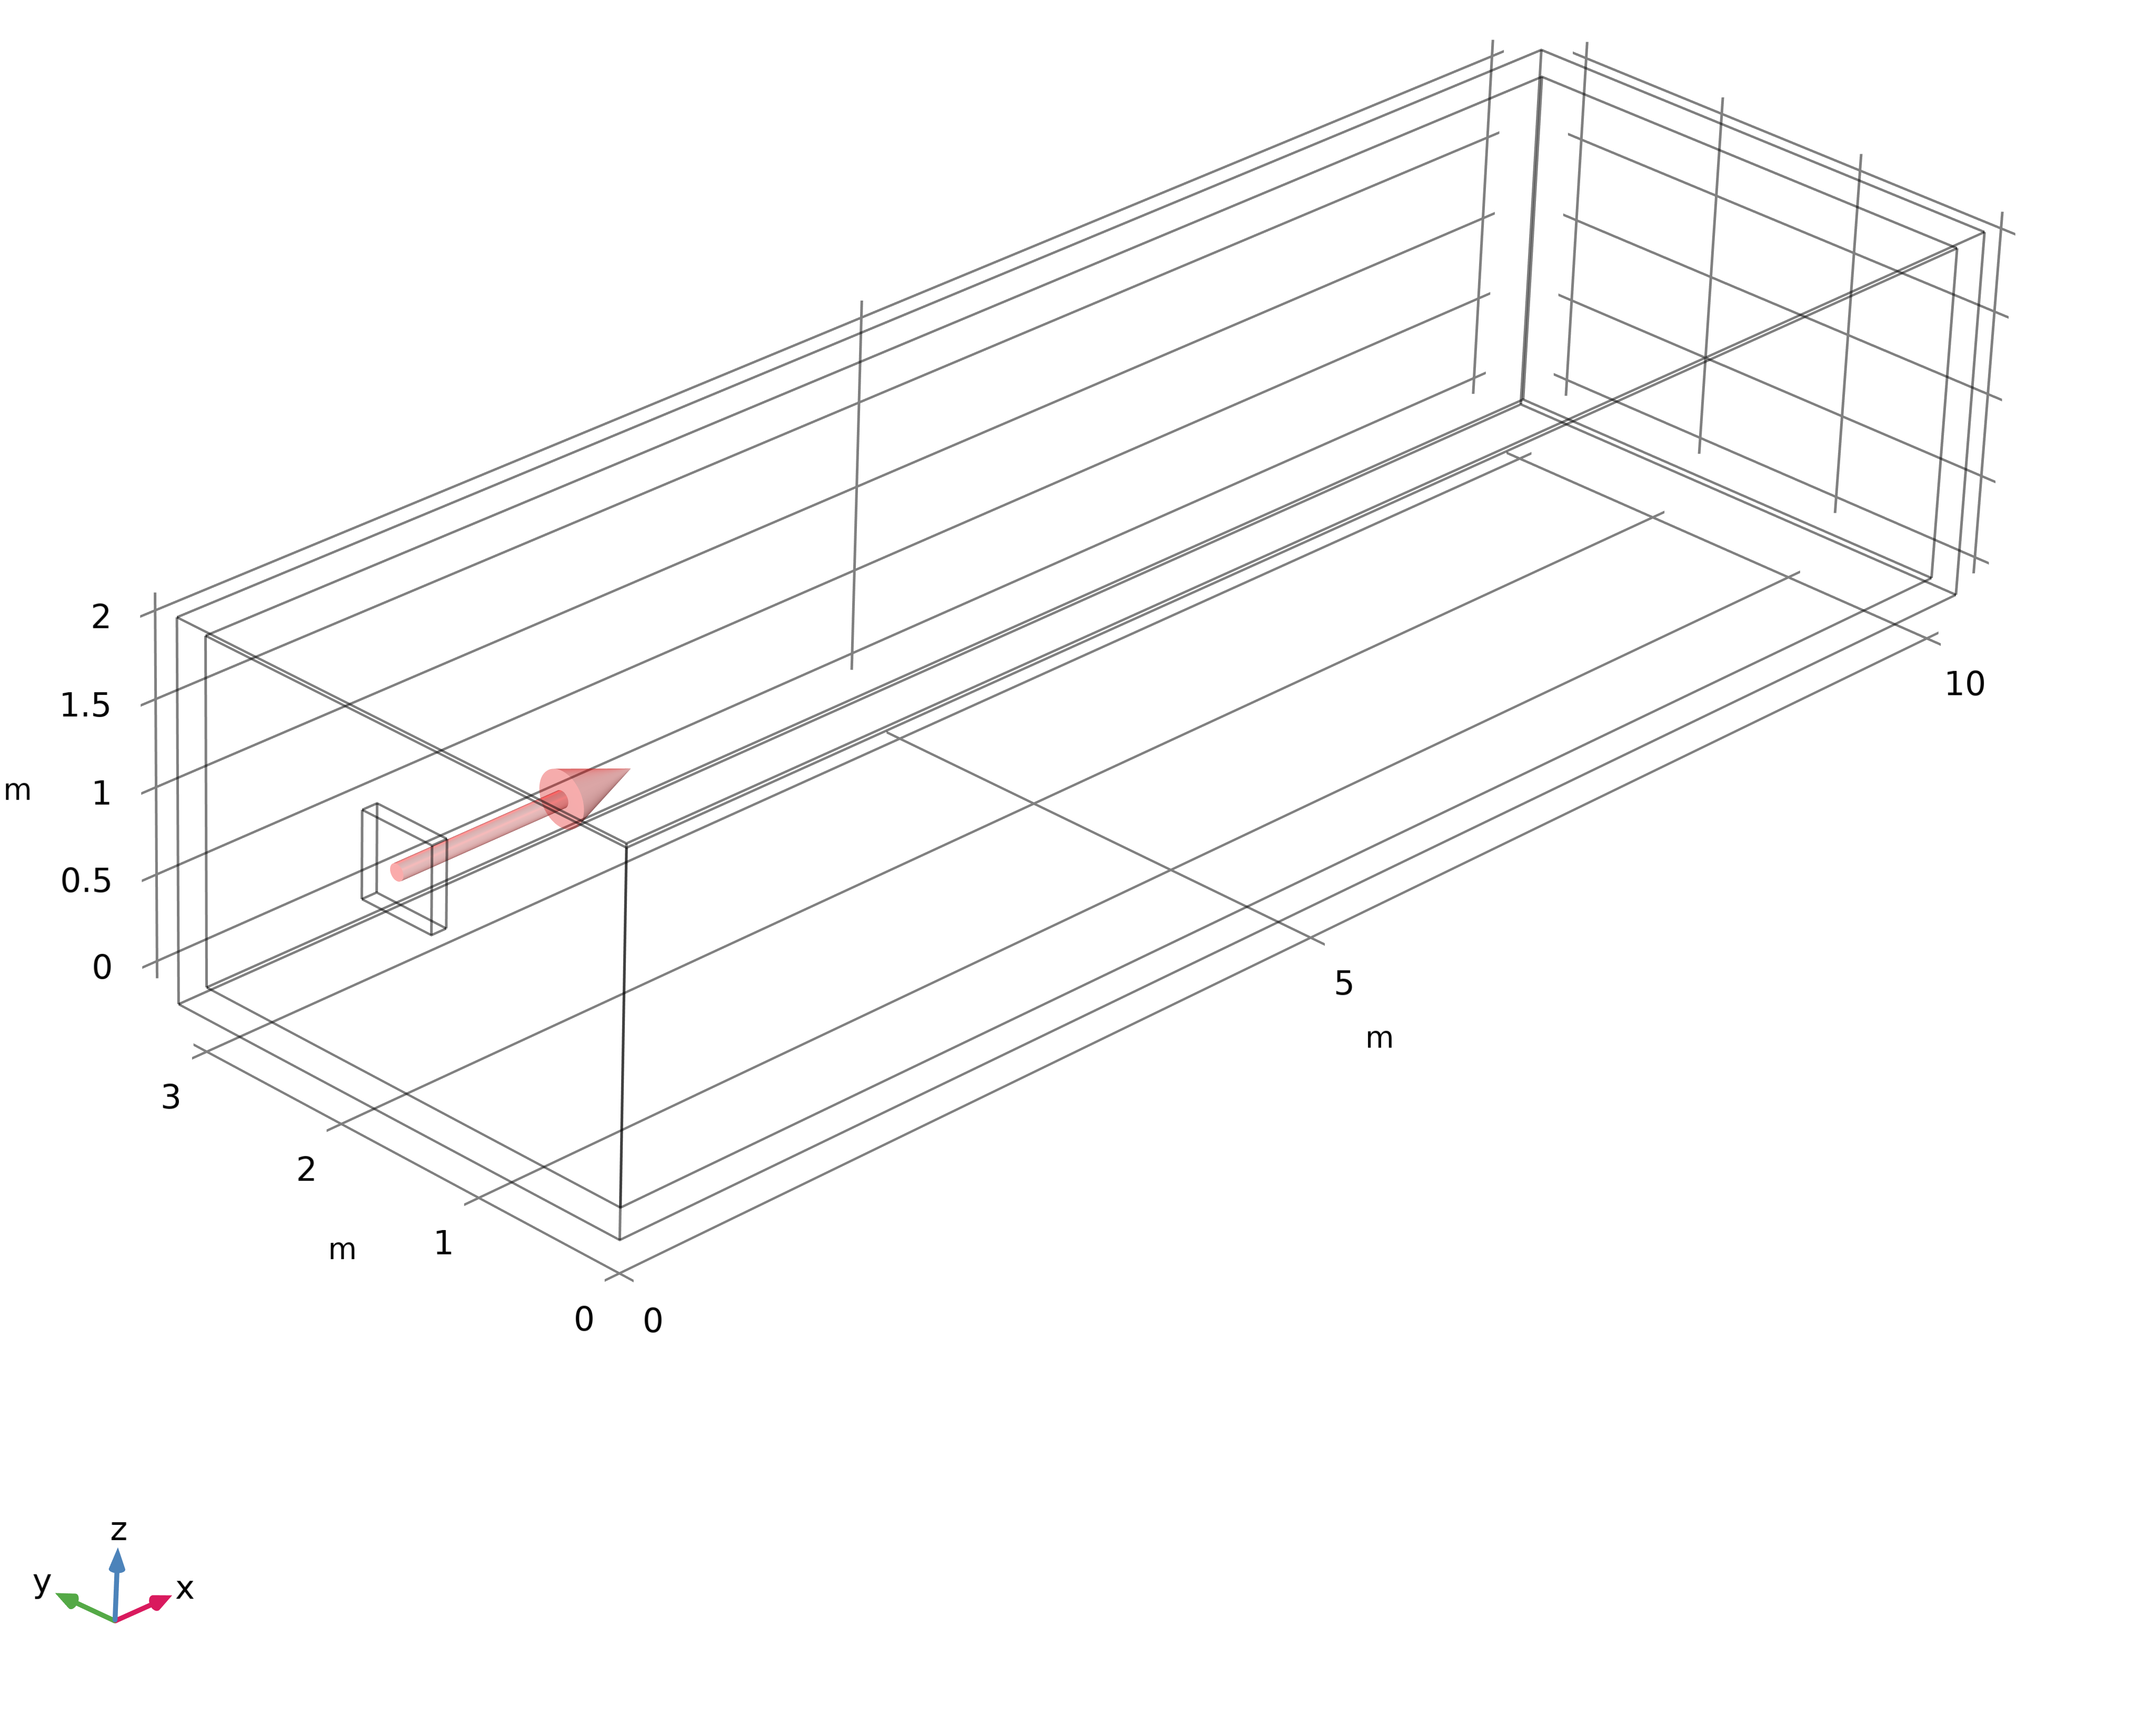
\includegraphics[width=10cm,height=9cm]{figures/Laminar flow schematic.png}
  \caption{Laminar flow schematic} % 层流示意图
  \label{Laminar flow schematic}
\end{figure}

When simulating the gas inside a greenhouse, laminar flow simulation can be used to predict the movement of the gas. According to the problem, the boundary conditions on one side of the greenhouse fan are set as velocity inlet conditions, while the outer glass and the bottom soil are set as wall conditions. In this way, we construct a laminar flow model for a crop-free greenhouse, below we give the specific boundary conditions and initial values. In COMSOL, we construct a crop-free laminar flow model as shown as illustrated in the schematic diagram\ref{{Laminar flow schematic}.  
initial values:
$$\left\{\begin{matrix} 
  P|_{t=0}=101.325 \\ 
  V|_{t=0}=0\\
  V_t|_{t=0}=0\\
\end{matrix}\right$$
boundary conditions:
$$\left\{\begin{matrix} 
  V_z|_{z=0}=V_z|_{z=2}=0\\
V_x|_{x=0}=V_x|_{x=3}=0\\
V_y|_{y=10}=0\\
V|_{y=0,x,z\in (1.25,1.75)}=2\vec{j} 
\end{matrix}\right$$
% 在模拟温室内气体时,层流模拟可以用于预测气体的运动,根据题目,温室风机一侧的边界条件设置为速度入口条件,外层玻璃和底土被设置为墙体条件,下面我们给出其具体边界条件和初始值。在comsol中我们构造了如图Missing close braceMissing close brace层流模型。

\subsubsection{Fluid heat transfer}
% 流体传热

Fluid heat transfer is the field that investigates how thermal energy is transferred within a fluid. This process typically involves the transfer of heat from one region to another, achieved through the movement or conduction of the fluid. There are several ways to describe fluid heat transfer:
% 流体传热是研究热能如何在流体中传递的领域。这个过程通常涉及热能从一个区域传递到另一个区域,通过流体的运动或传导来实现。有几种方式可以描述流体传热:
\begin{enumerate}
	\item Convection heat transfer: This is the process of transferring thermal energy through the movement of a fluid. When the fluid flows over the surface of an object, it carries away heat from the surface, and this is convection heat transfer. This process is typically influenced by the velocity, density, and temperature differences of the fluid.
% 对流传热: 这是通过流体的流动来传递热能的过程。当流体在物体表面流动时,它带走了表面的热量,这就是对流传热。这个过程通常由流体的速度、密度和温度差异来影响。

  \item Conduction heat transfer: This is the process of transferring heat through the internal molecular vibrations of a substance. In fluids, this often refers to the direct collision and transfer of thermal energy between molecules.
% 传导传热: 这是通过物质内部的分子振动来传递热量的过程。在流体中,这通常是指分子之间的直接碰撞传递热能。

    \item Radiation heat transfer: This is the process of transferring heat through electromagnetic radiation, independent of the material of the fluid. Thermal radiation can propagate through a vacuum without the need for a medium.
% 辐射传热: 这是通过电磁辐射传递热量的过程,与流体的物质无关。热辐射可以在真空中传递,而不需要介质。
\end{enumerate}

Regarding this issue, since the model does not account for solar radiation, the entire greenhouse primarily relies on convective heat exchange and conductive energy transfer.
% 对于这个问题由于该模型不考虑太阳辐射,整个温室主要是通过对流换热和传导交换能量。

\subsubsection{Multiphysics field coupling}
% 多物理场耦合

By using computational fluid dynamics (CFD) methods, we can simulate the airflow when warm air is introduced. Since the flow is laminar, meaning the fluid exhibits clear layering in the flow direction, we can observe relatively ordered flow patterns.
% 通过使用流体力学的方法,我们可以模拟暖风通入时的空气运动。由于流动是层流的,即流体在流动方向上的层次结构清晰,我们可以观察到相对有序的流动模式。

Considering fluid heat transfer is crucial for analyzing changes in temperature distribution within the greenhouse. We are interested in understanding how heat is transferred within the greenhouse. Heat transfer mechanisms include convective heat transfer and conductive heat transfer. When warm air enters the greenhouse, convective heat transfer is the primary mechanism at play.
% 考虑流体传热对于分析温室内温度分布的变化至关重要,我们关心热量是如何在温室内传递的。传热机制包括对流传热、和传导传热。当暖风进入温室时,对流传热是主要的机制。

We couple fluid dynamics and heat transfer to simulate the airflow and temperature changes induced by warm air. By employing tools such as Computational Fluid Dynamics (CFD) and Finite Element Analysis (FEA), we can gain a more detailed understanding of the velocity and temperature distribution when warm air is introduced.
% 我们将流体力学和传热学耦合在一起,以模拟暖风引发的空气流动和温度变化。通过使用计算流体力学(CFD)和有限元分析(FEA)等工具,我们可以更详细地了解暖风通入时风速和温度分布。

By comprehensively considering these physical fields, we can gain a more comprehensive understanding of non-isothermal flow phenomena. Solving for multiple physical fields allows us to obtain the temperature and wind speed distribution in a crop-free glass greenhouse.
% 通过综合考虑这些物理场,我们可以更全面地了解非等温流动的现象,通过对多物理场的求解我们可以得到无作物玻璃温室温度和风速分布。

\subsubsection{Crop-free glass greenhouse simulation}


% 两张图片并列
\begin{figure}[htbp]
      \centering
      \subfigure[Crop-free Greenhouse Geometric Model] {
          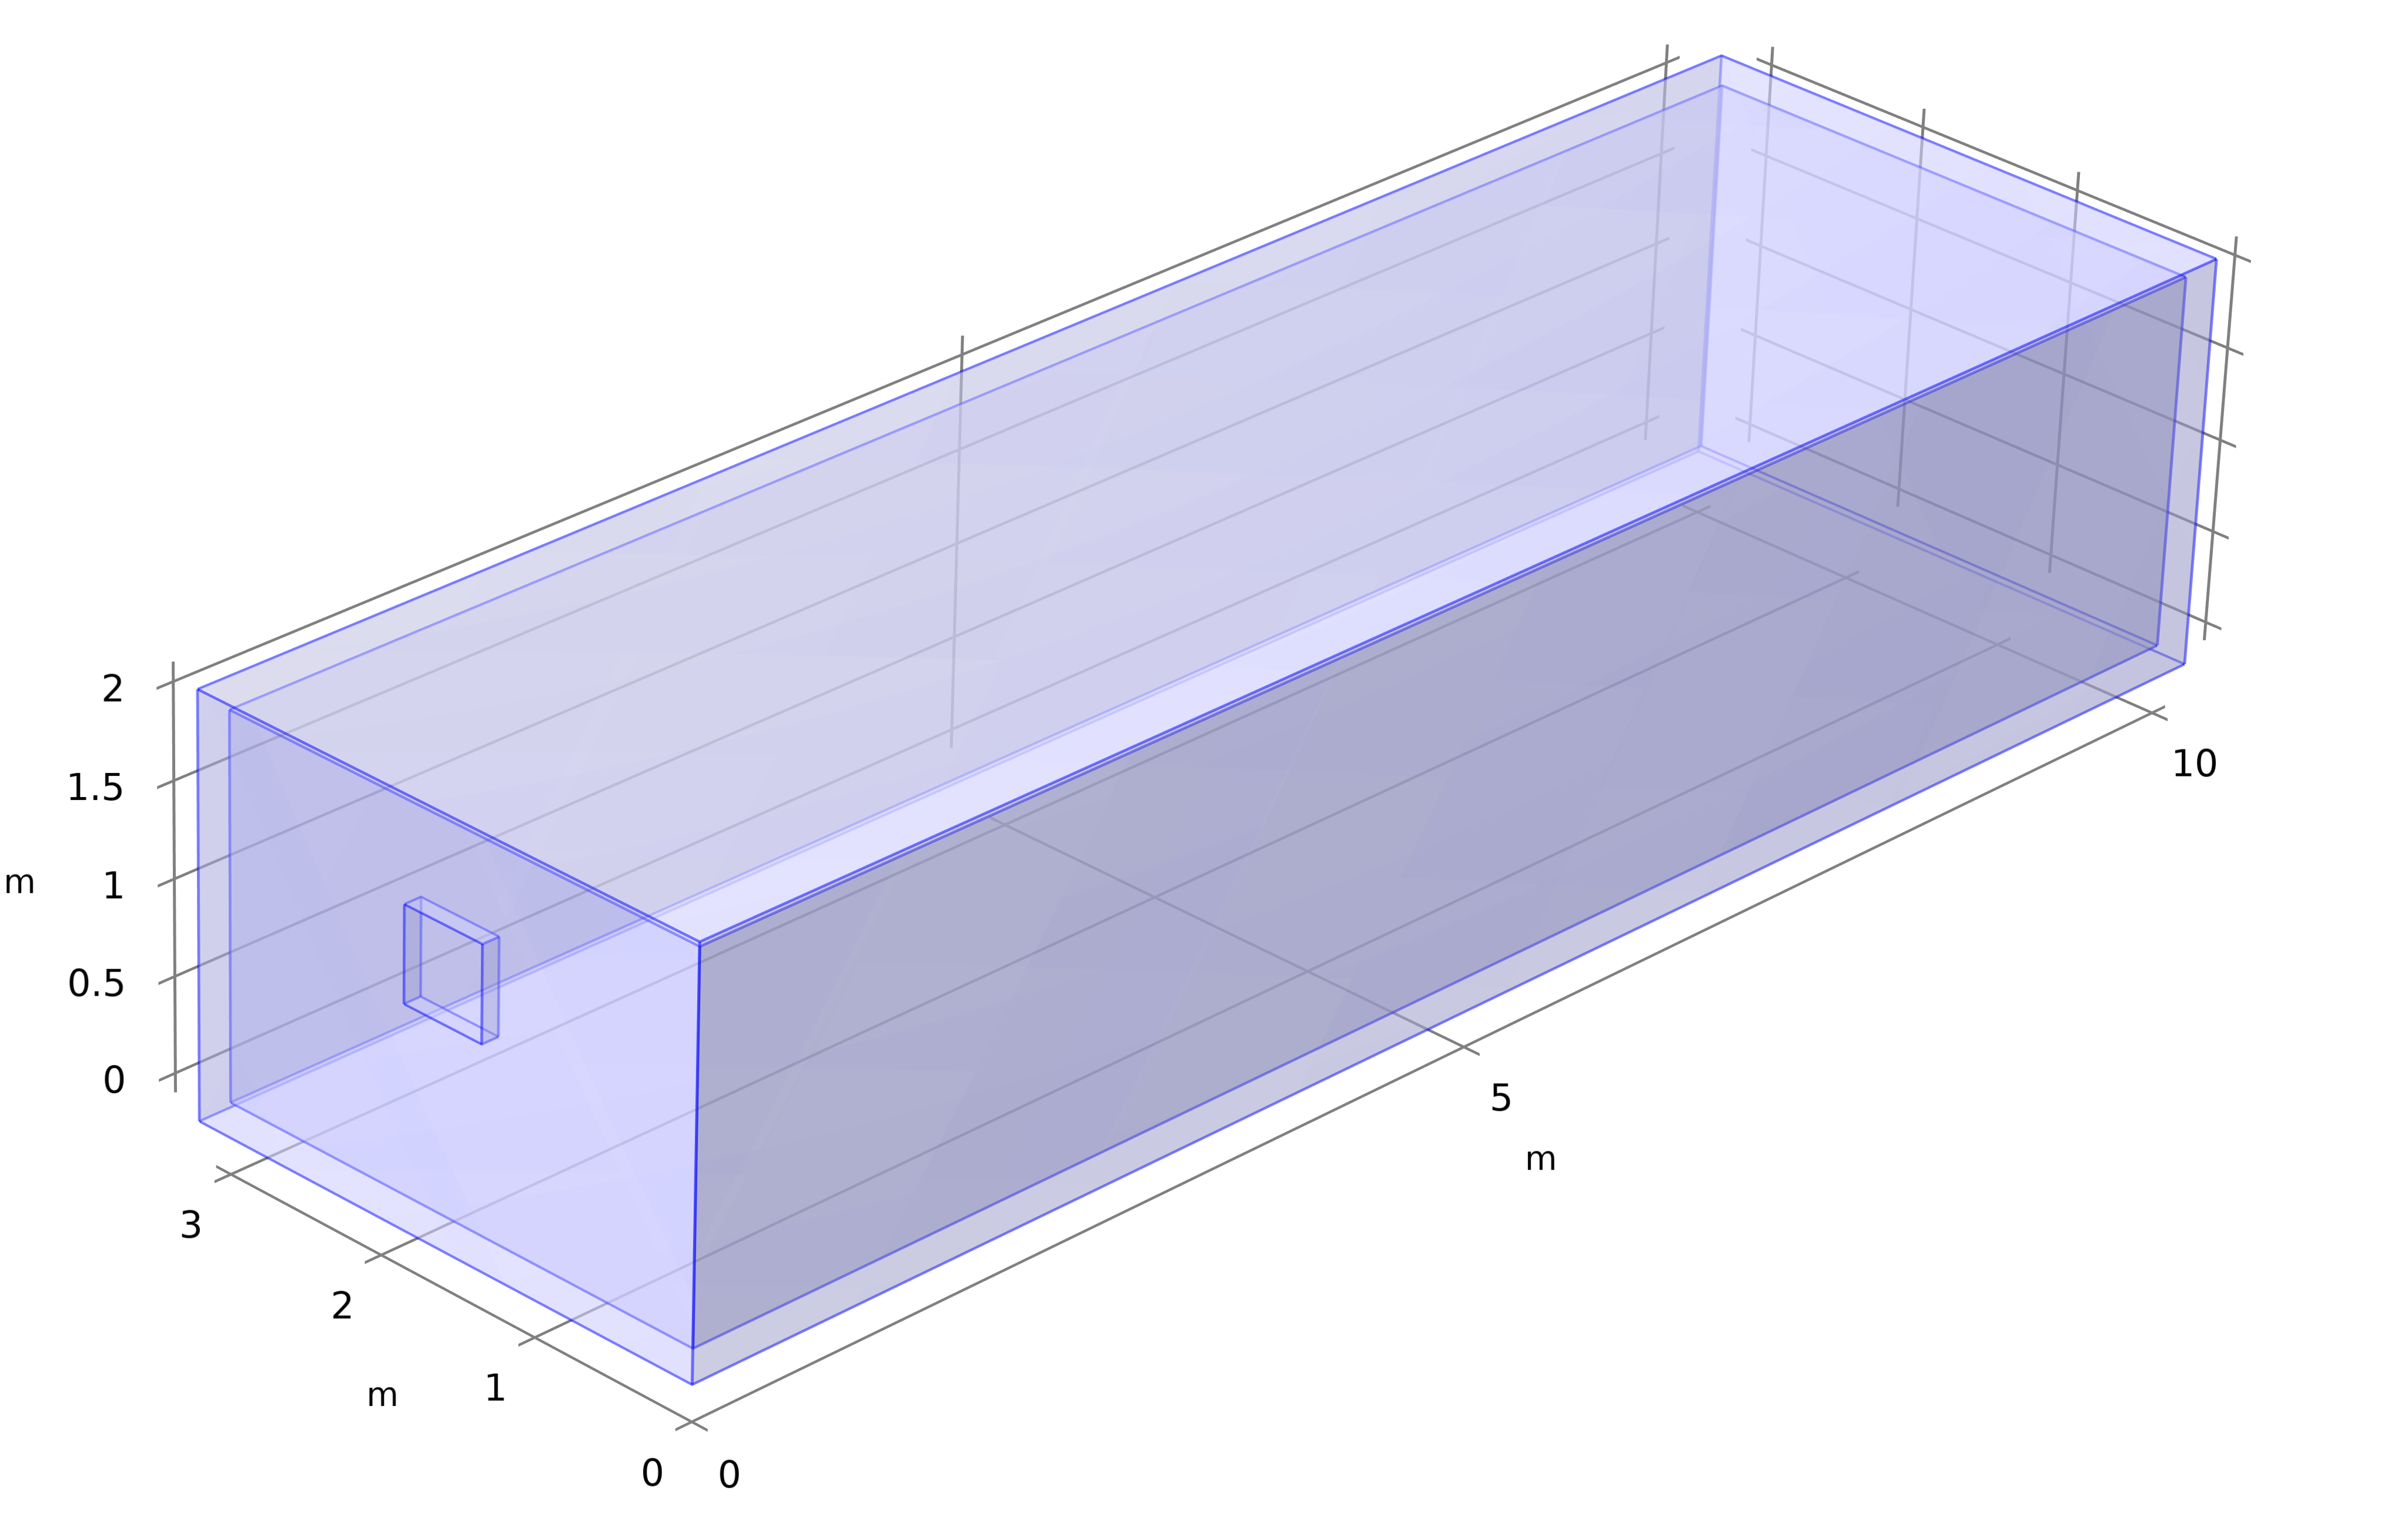
\includegraphics[width=0.4\textwidth]{figures/model1.png}
          \label{Crop-free Greenhouse Geometric Model}
      }
       \subfigure[Parameter Settings] { \label{Crop-free Greenhouse Geometric Model}
         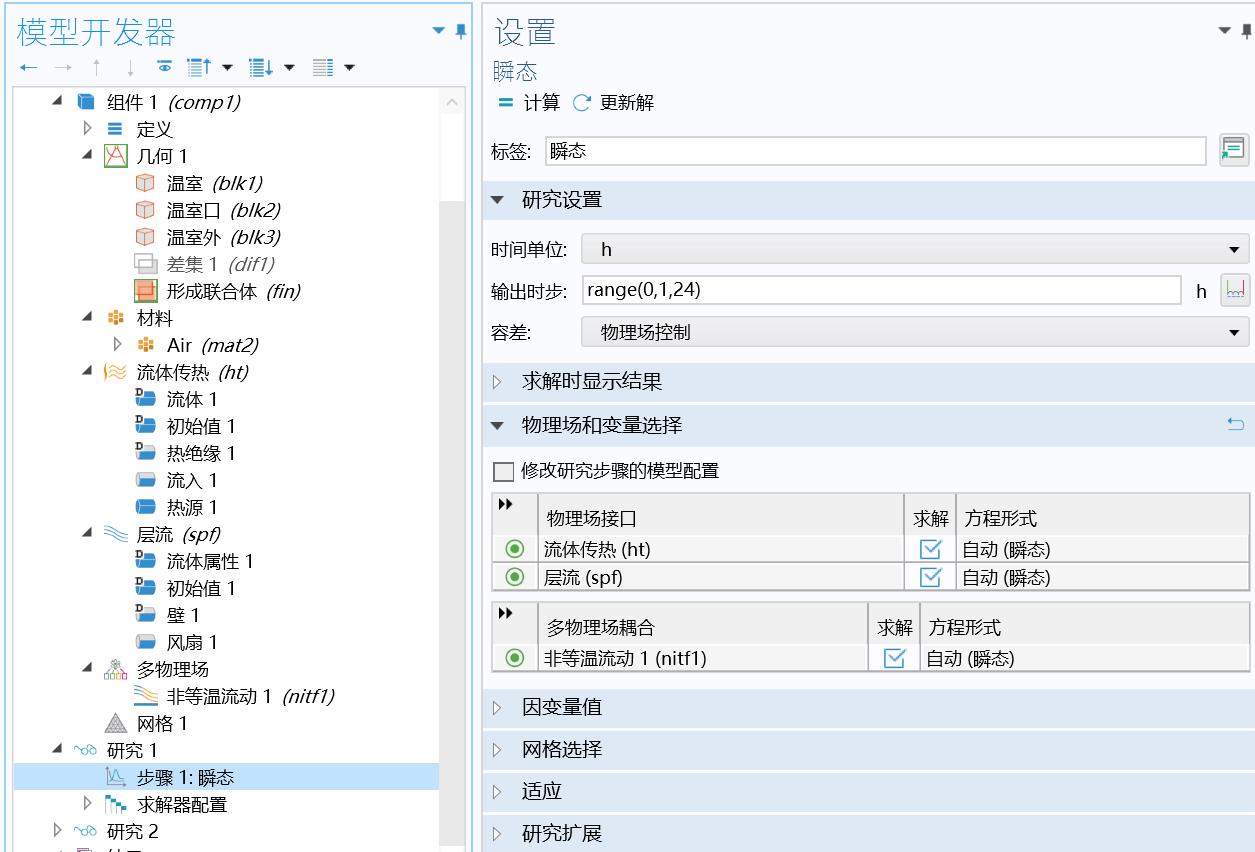
\includegraphics[width=0.4\textwidth]{figures/setting1.png}
          \label{Parameter Settings}% 参数设置
      }
      
      \caption{Preparation for Crop-Free Simulation} %无作物仿真准备工作
      \label{Preparation for Crop-Free Simulation}
  \end{figure}

  We conducted simulations using COMSOL. Firstly, following the given problem statement, we constructed the geometric model of a crop-free glass greenhouse, as shown in Figure \ref{Crop-free Greenhouse Geometric Model}. Then, we set the parameters for fluid heat transfer, laminar flow, and non-isothermal flow, as illustrated in Figure \ref{Parameter Settings}. Subsequently, we performed the simulation calculations, and the convergence plot is presented in Figure \ref{Convergence Plot for the Crop-Free Greenhouse}. Finally, we obtained the temperature and wind speed distribution in the greenhouse, as depicted in Figure \ref{Plot for the Crop-Free Greenhouse}. As per the problem requirements, we extracted the results at a height of 0.5 meters, with specific data detailed in Figure \ref{Plot at 0.5m Cross-Section of the Crop-Free Greenhouse}.
% 我们使用comsol进行仿真,首先根据题意,我们构造了无作物玻璃温室的几何模型,模型如图\ref{},在设置流体传热,层流,非等温流动的参数如图\ref{},进行仿真计算,计算的收敛图见图\ref{},最后求出温室的温度与风速分布,如图/ref{},根据题意,我们截取了0.5m高度的结果,具体结果如图/ref{}.

% 两张图片并列
\begin{figure}[htbp]
      
      \centering
      \subfigure[Convergence Plot 1 for the Crop-Free Greenhouse] { 
          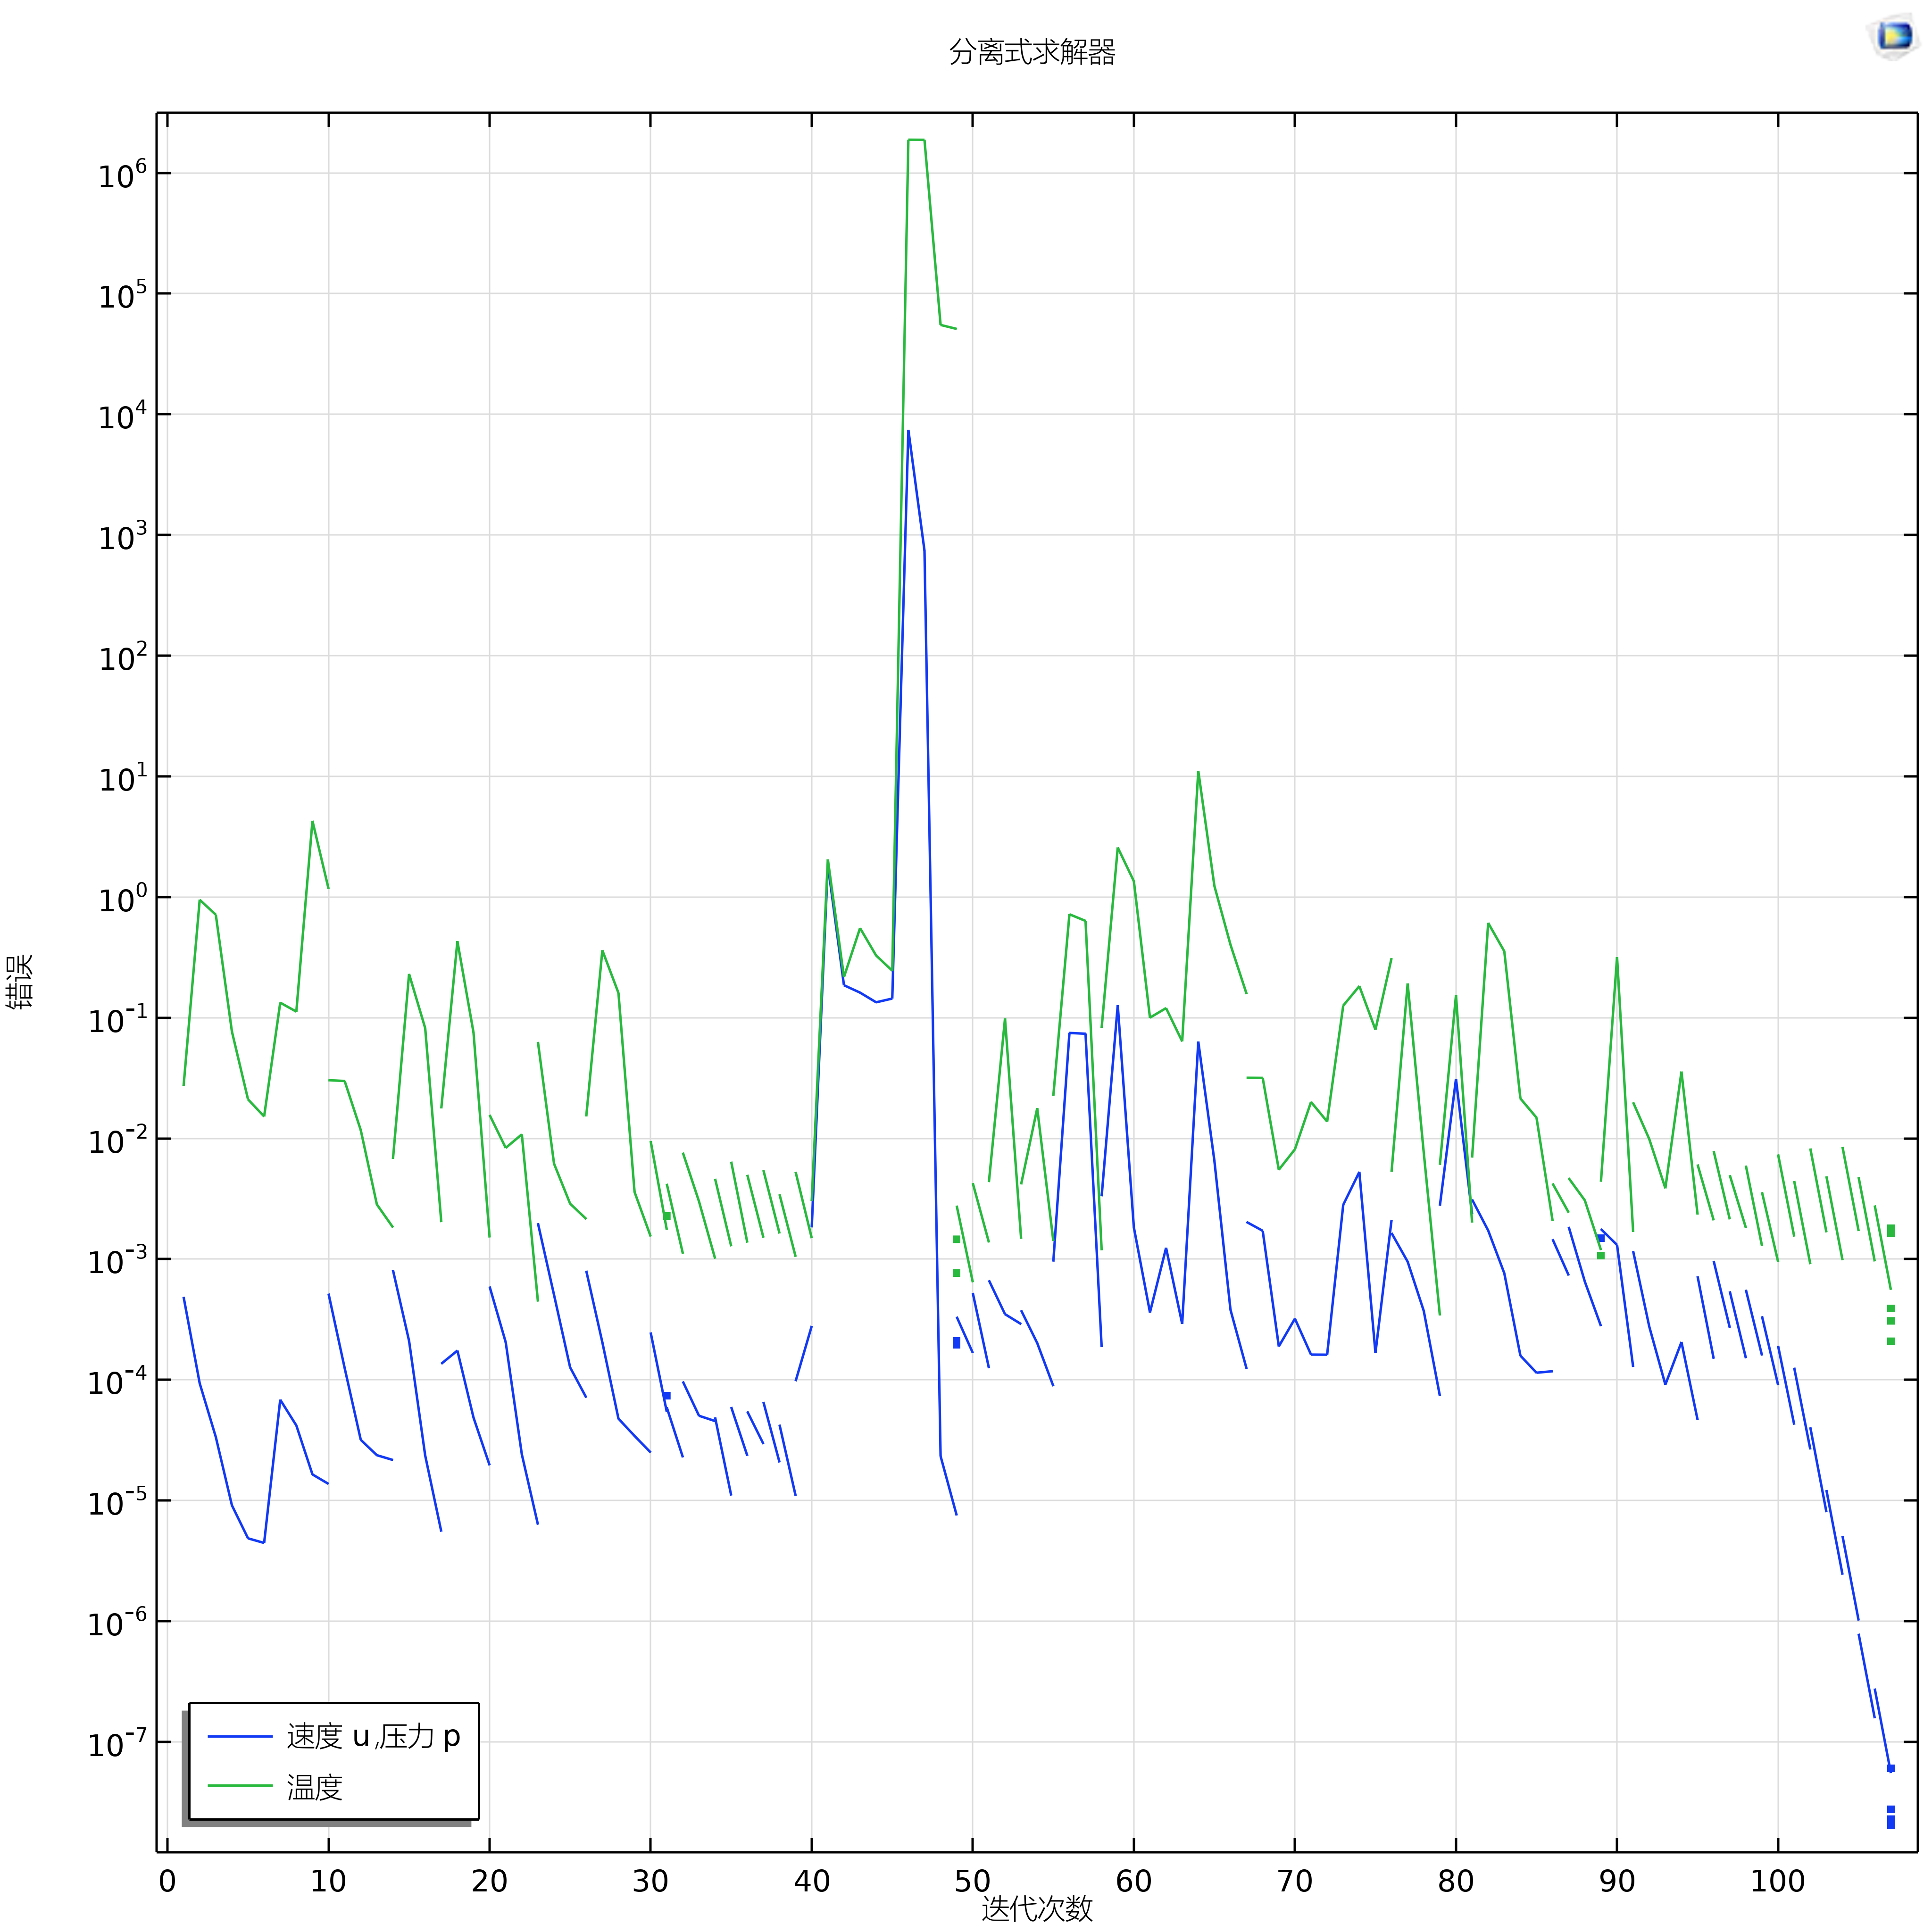
\includegraphics[width=0.4\textwidth]{figures/Model1 convergence plot1.png}
          
      }
       \subfigure[Convergence Plot 2 for the Crop-Free Greenhouse] {
         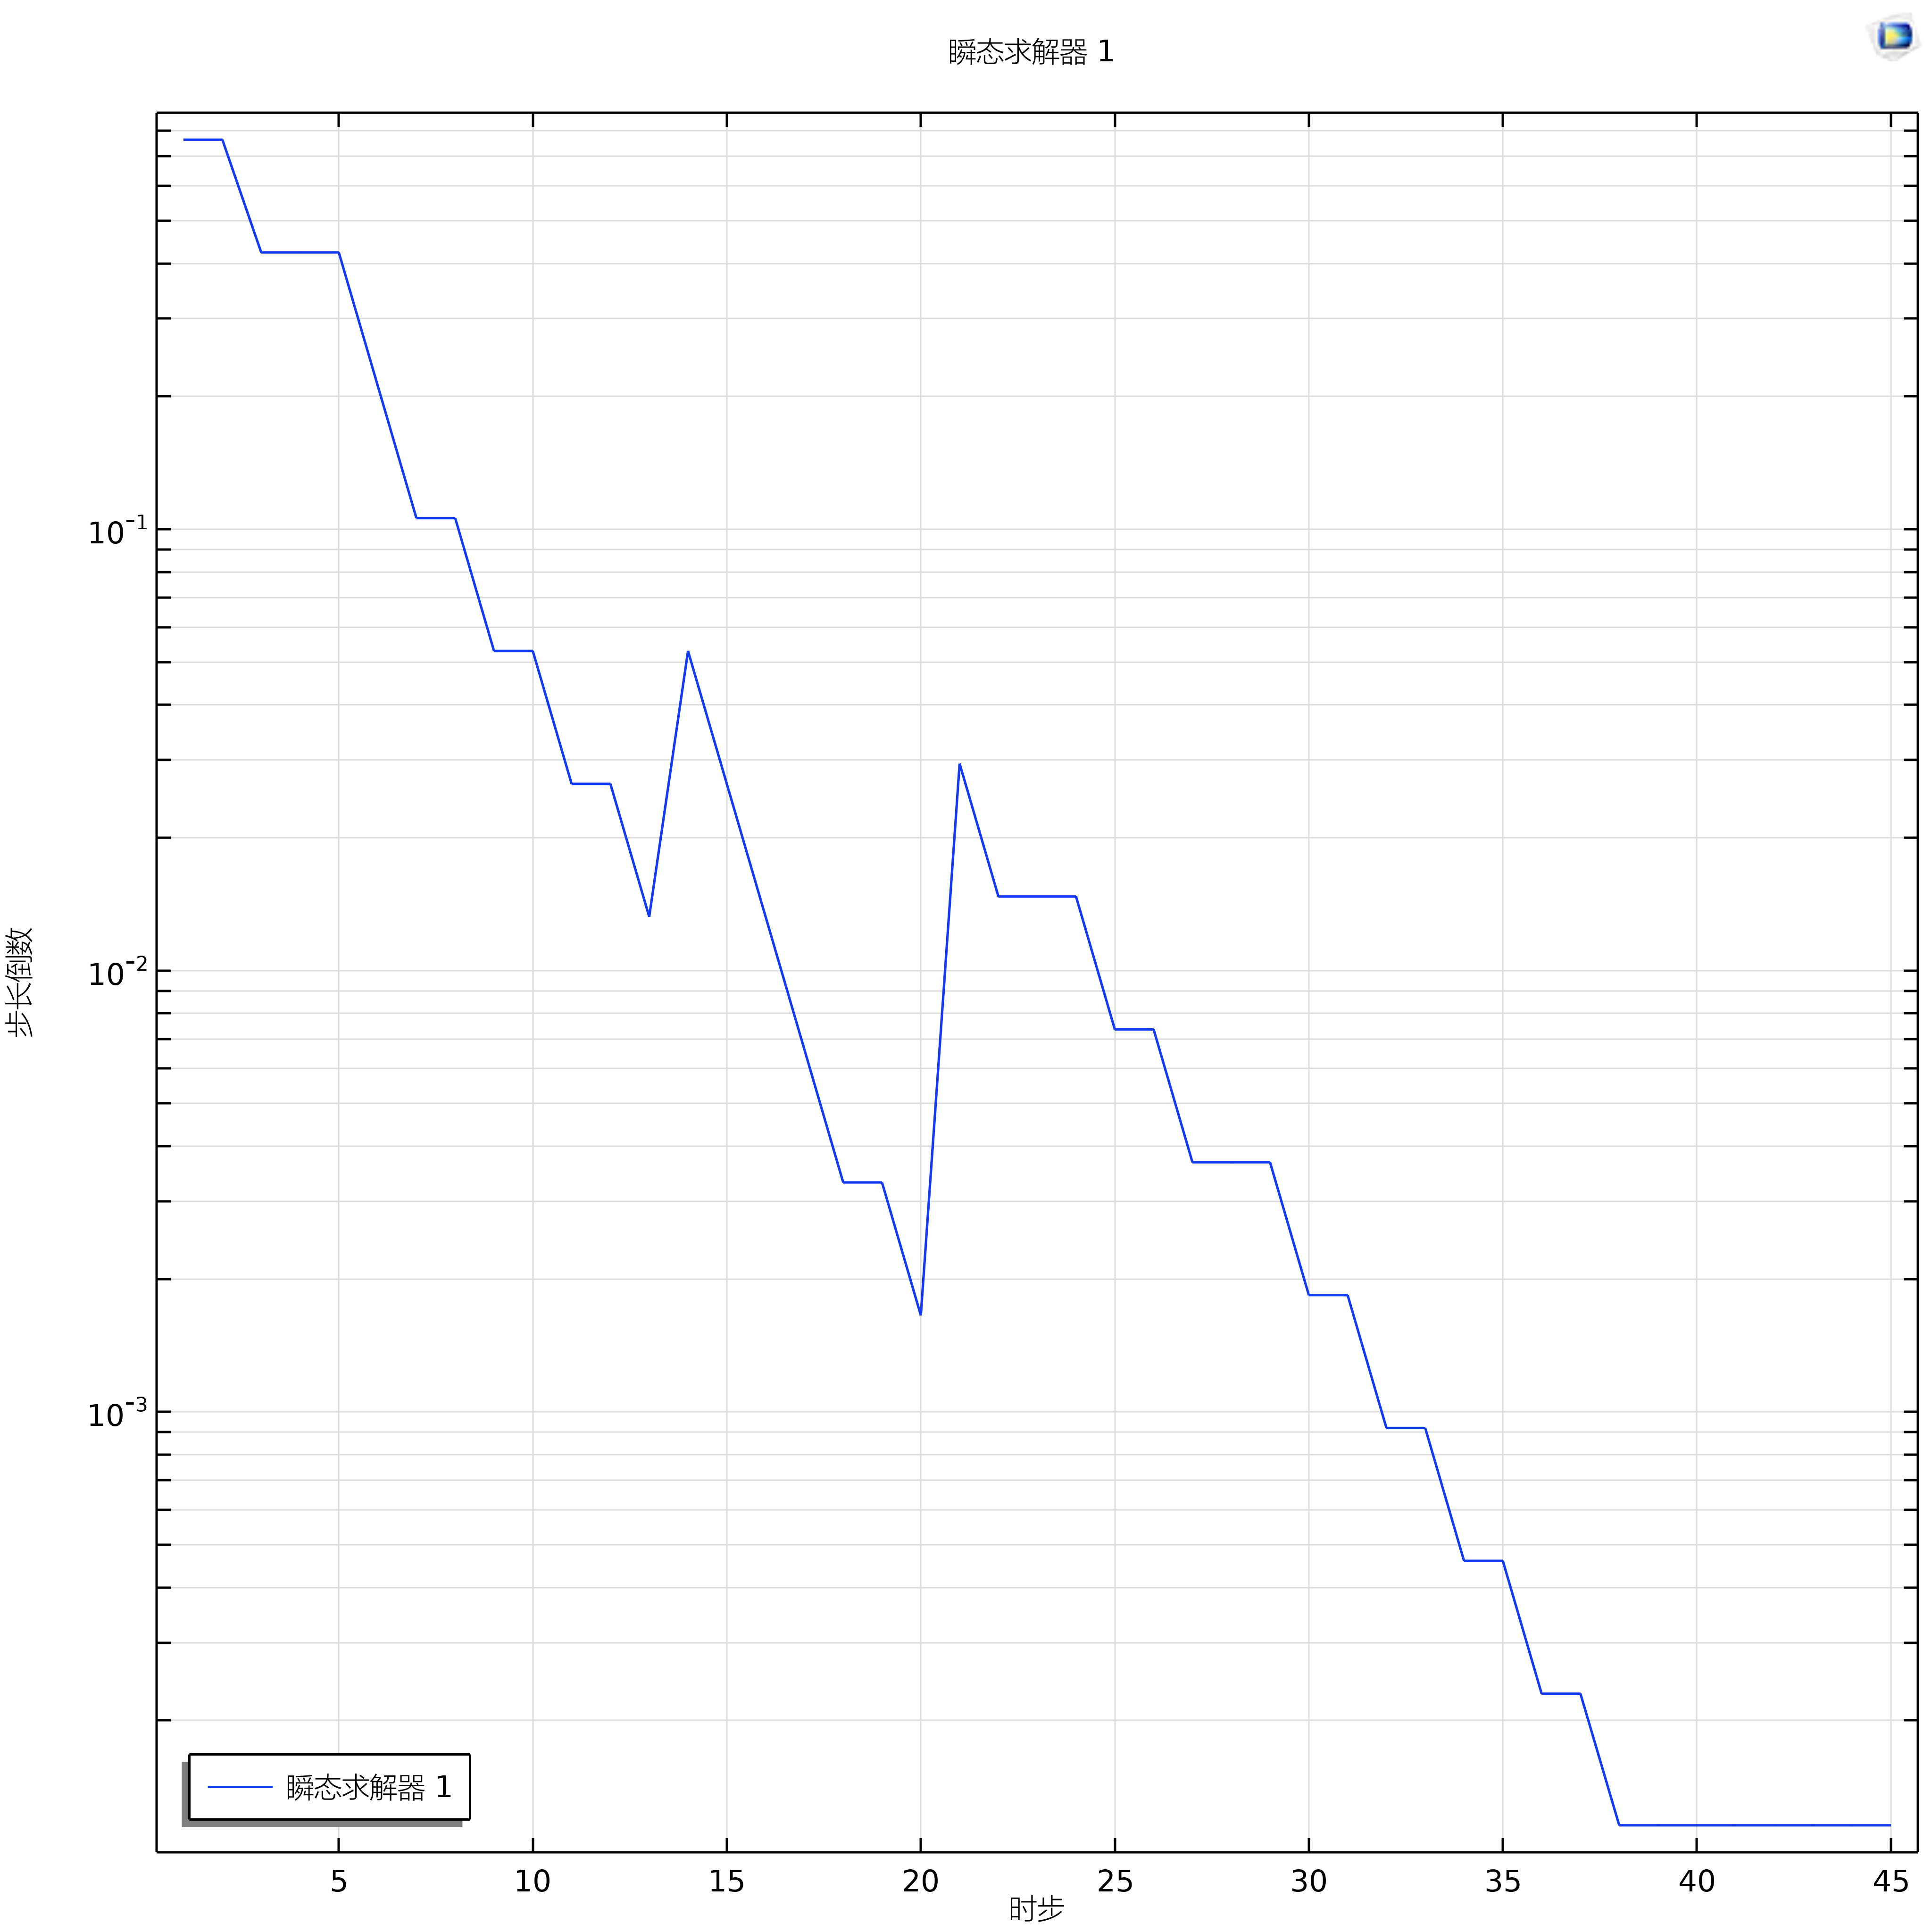
\includegraphics[width=0.4\textwidth]{figures/Model1 convergence plot2.png}
      }
      \caption{Convergence Plot for the Crop-Free Greenhouse}
      \label{Convergence Plot for the Crop-Free Greenhouse}
  \end{figure}

  
% 两张图片并列
\begin{figure}[htbp]
      
      \centering
      \subfigure[Crop-free glass greenhouse temperature] { 
          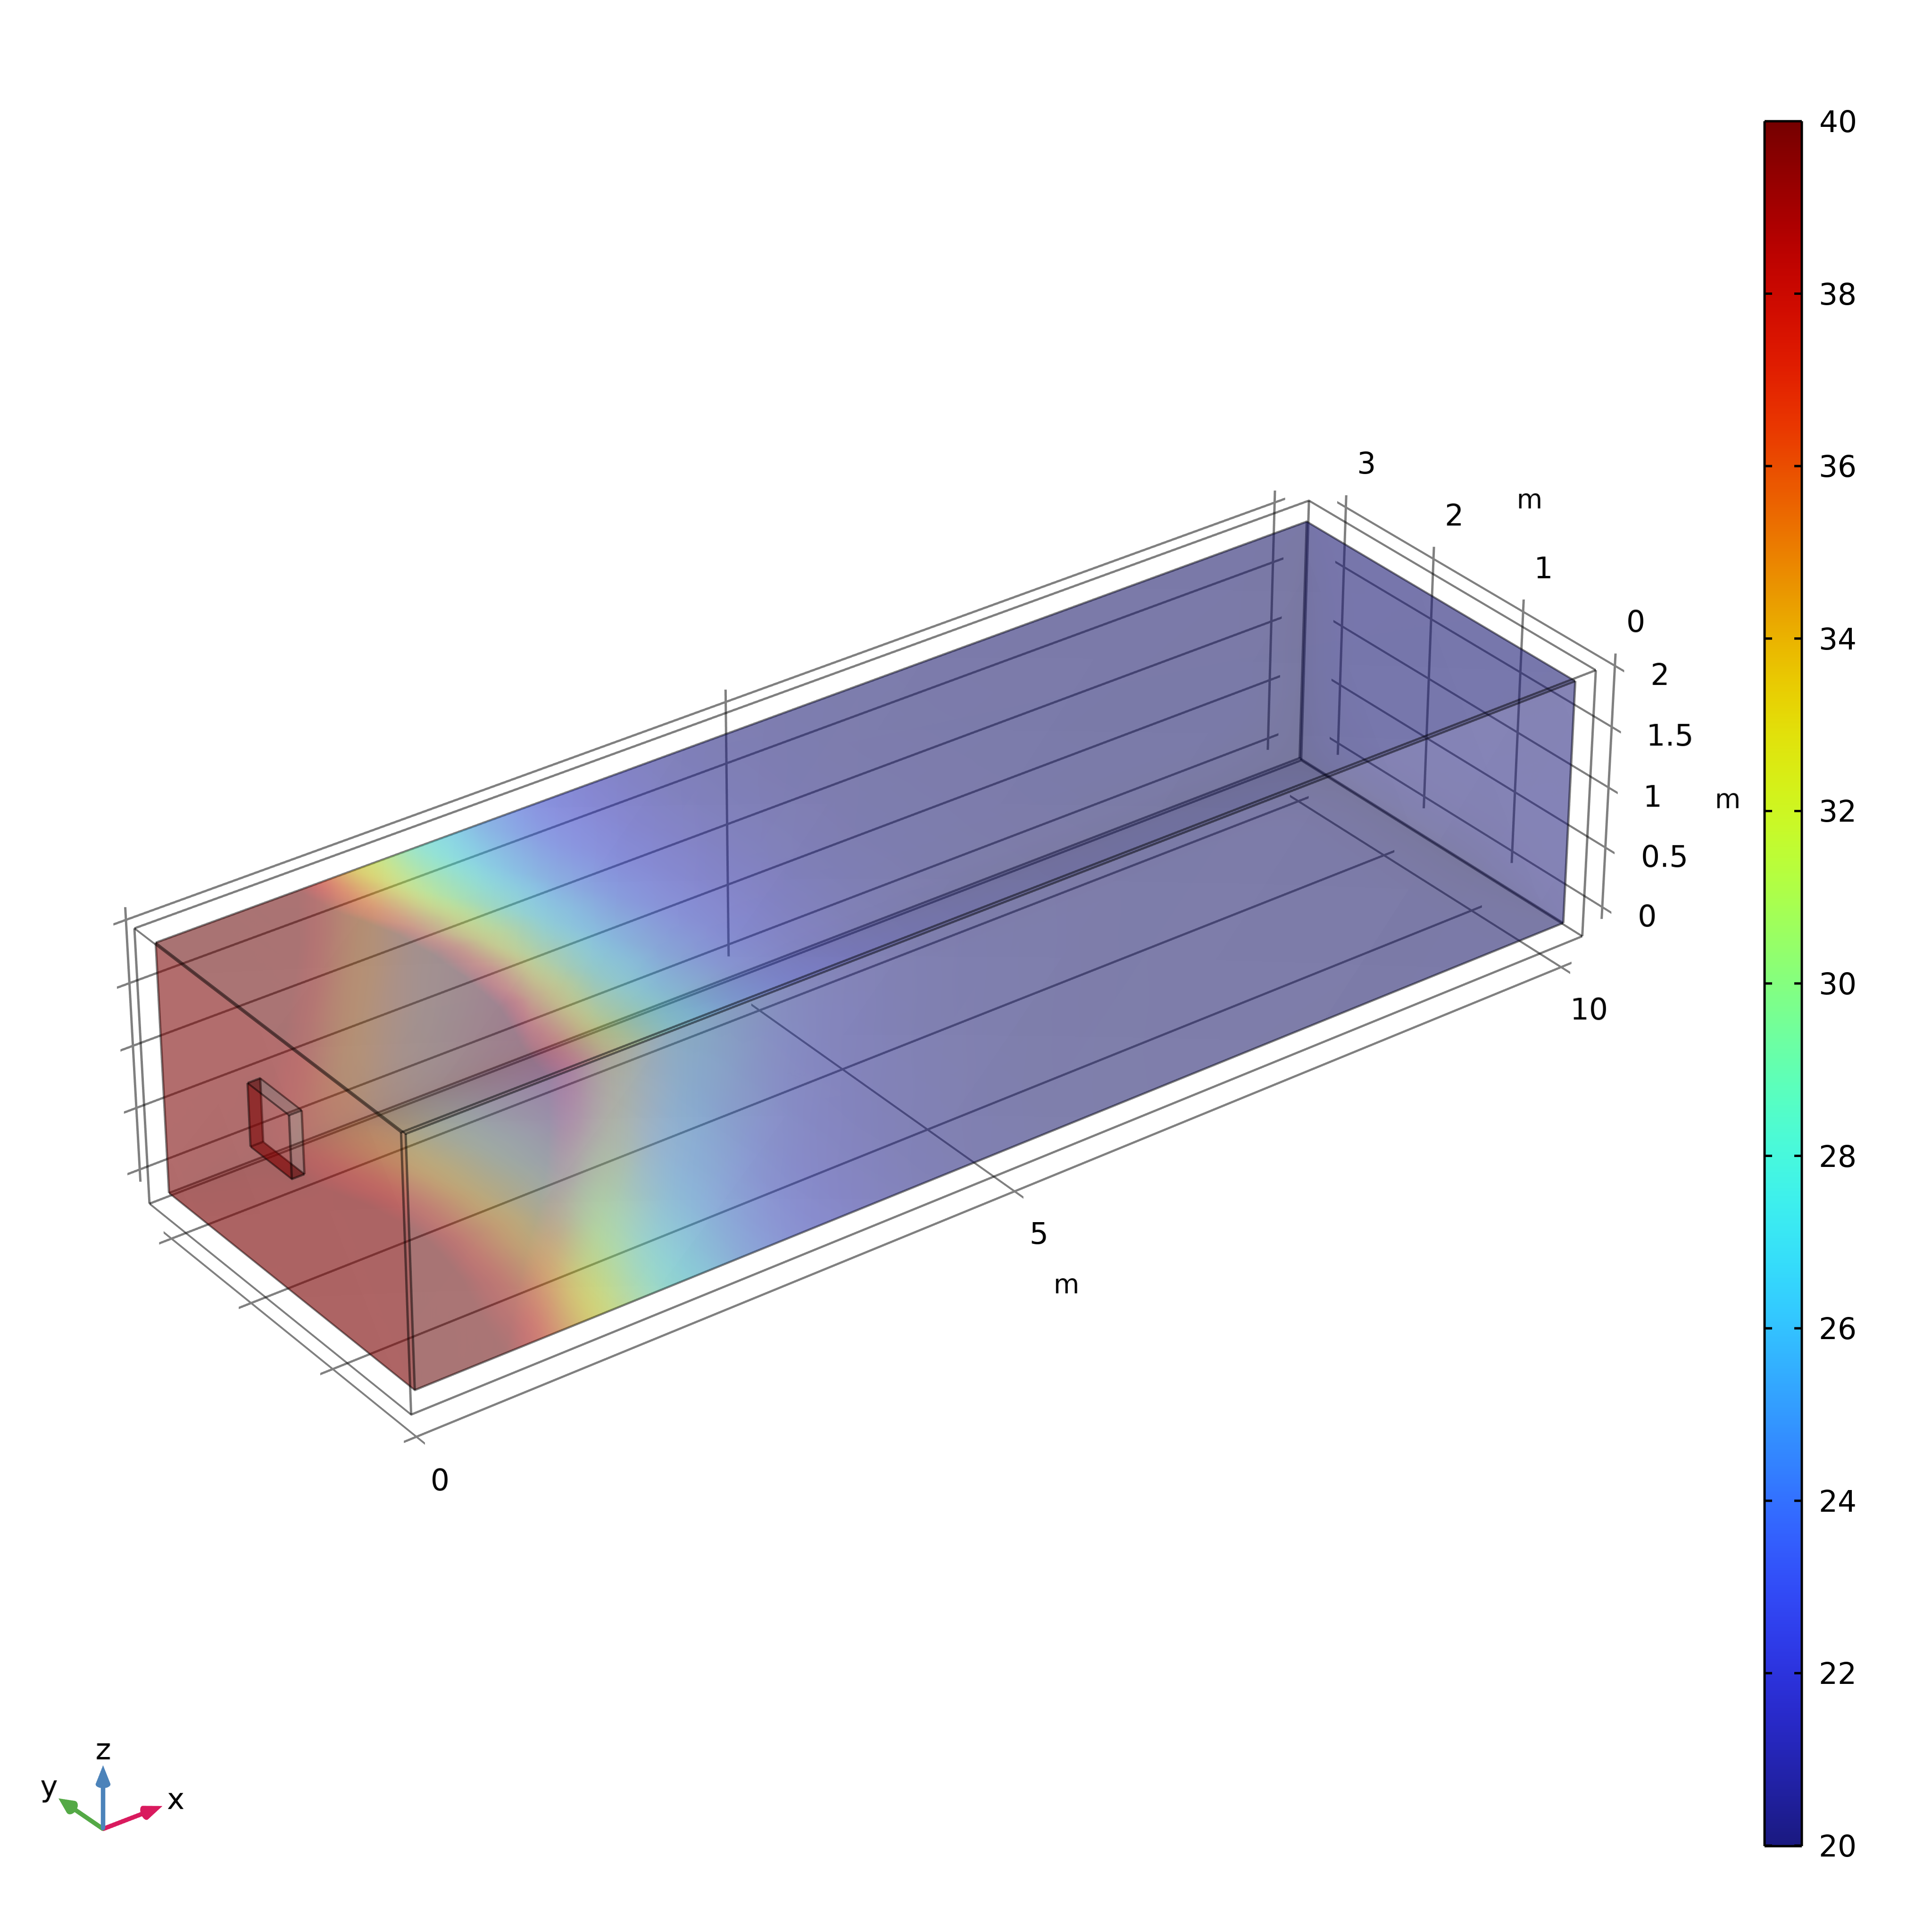
\includegraphics[width=0.4\textwidth]{figures/Crop-free glass greenhouse temperature.png}
          
      }
       \subfigure[Crop-free glass greenhouse wind speed] { 
         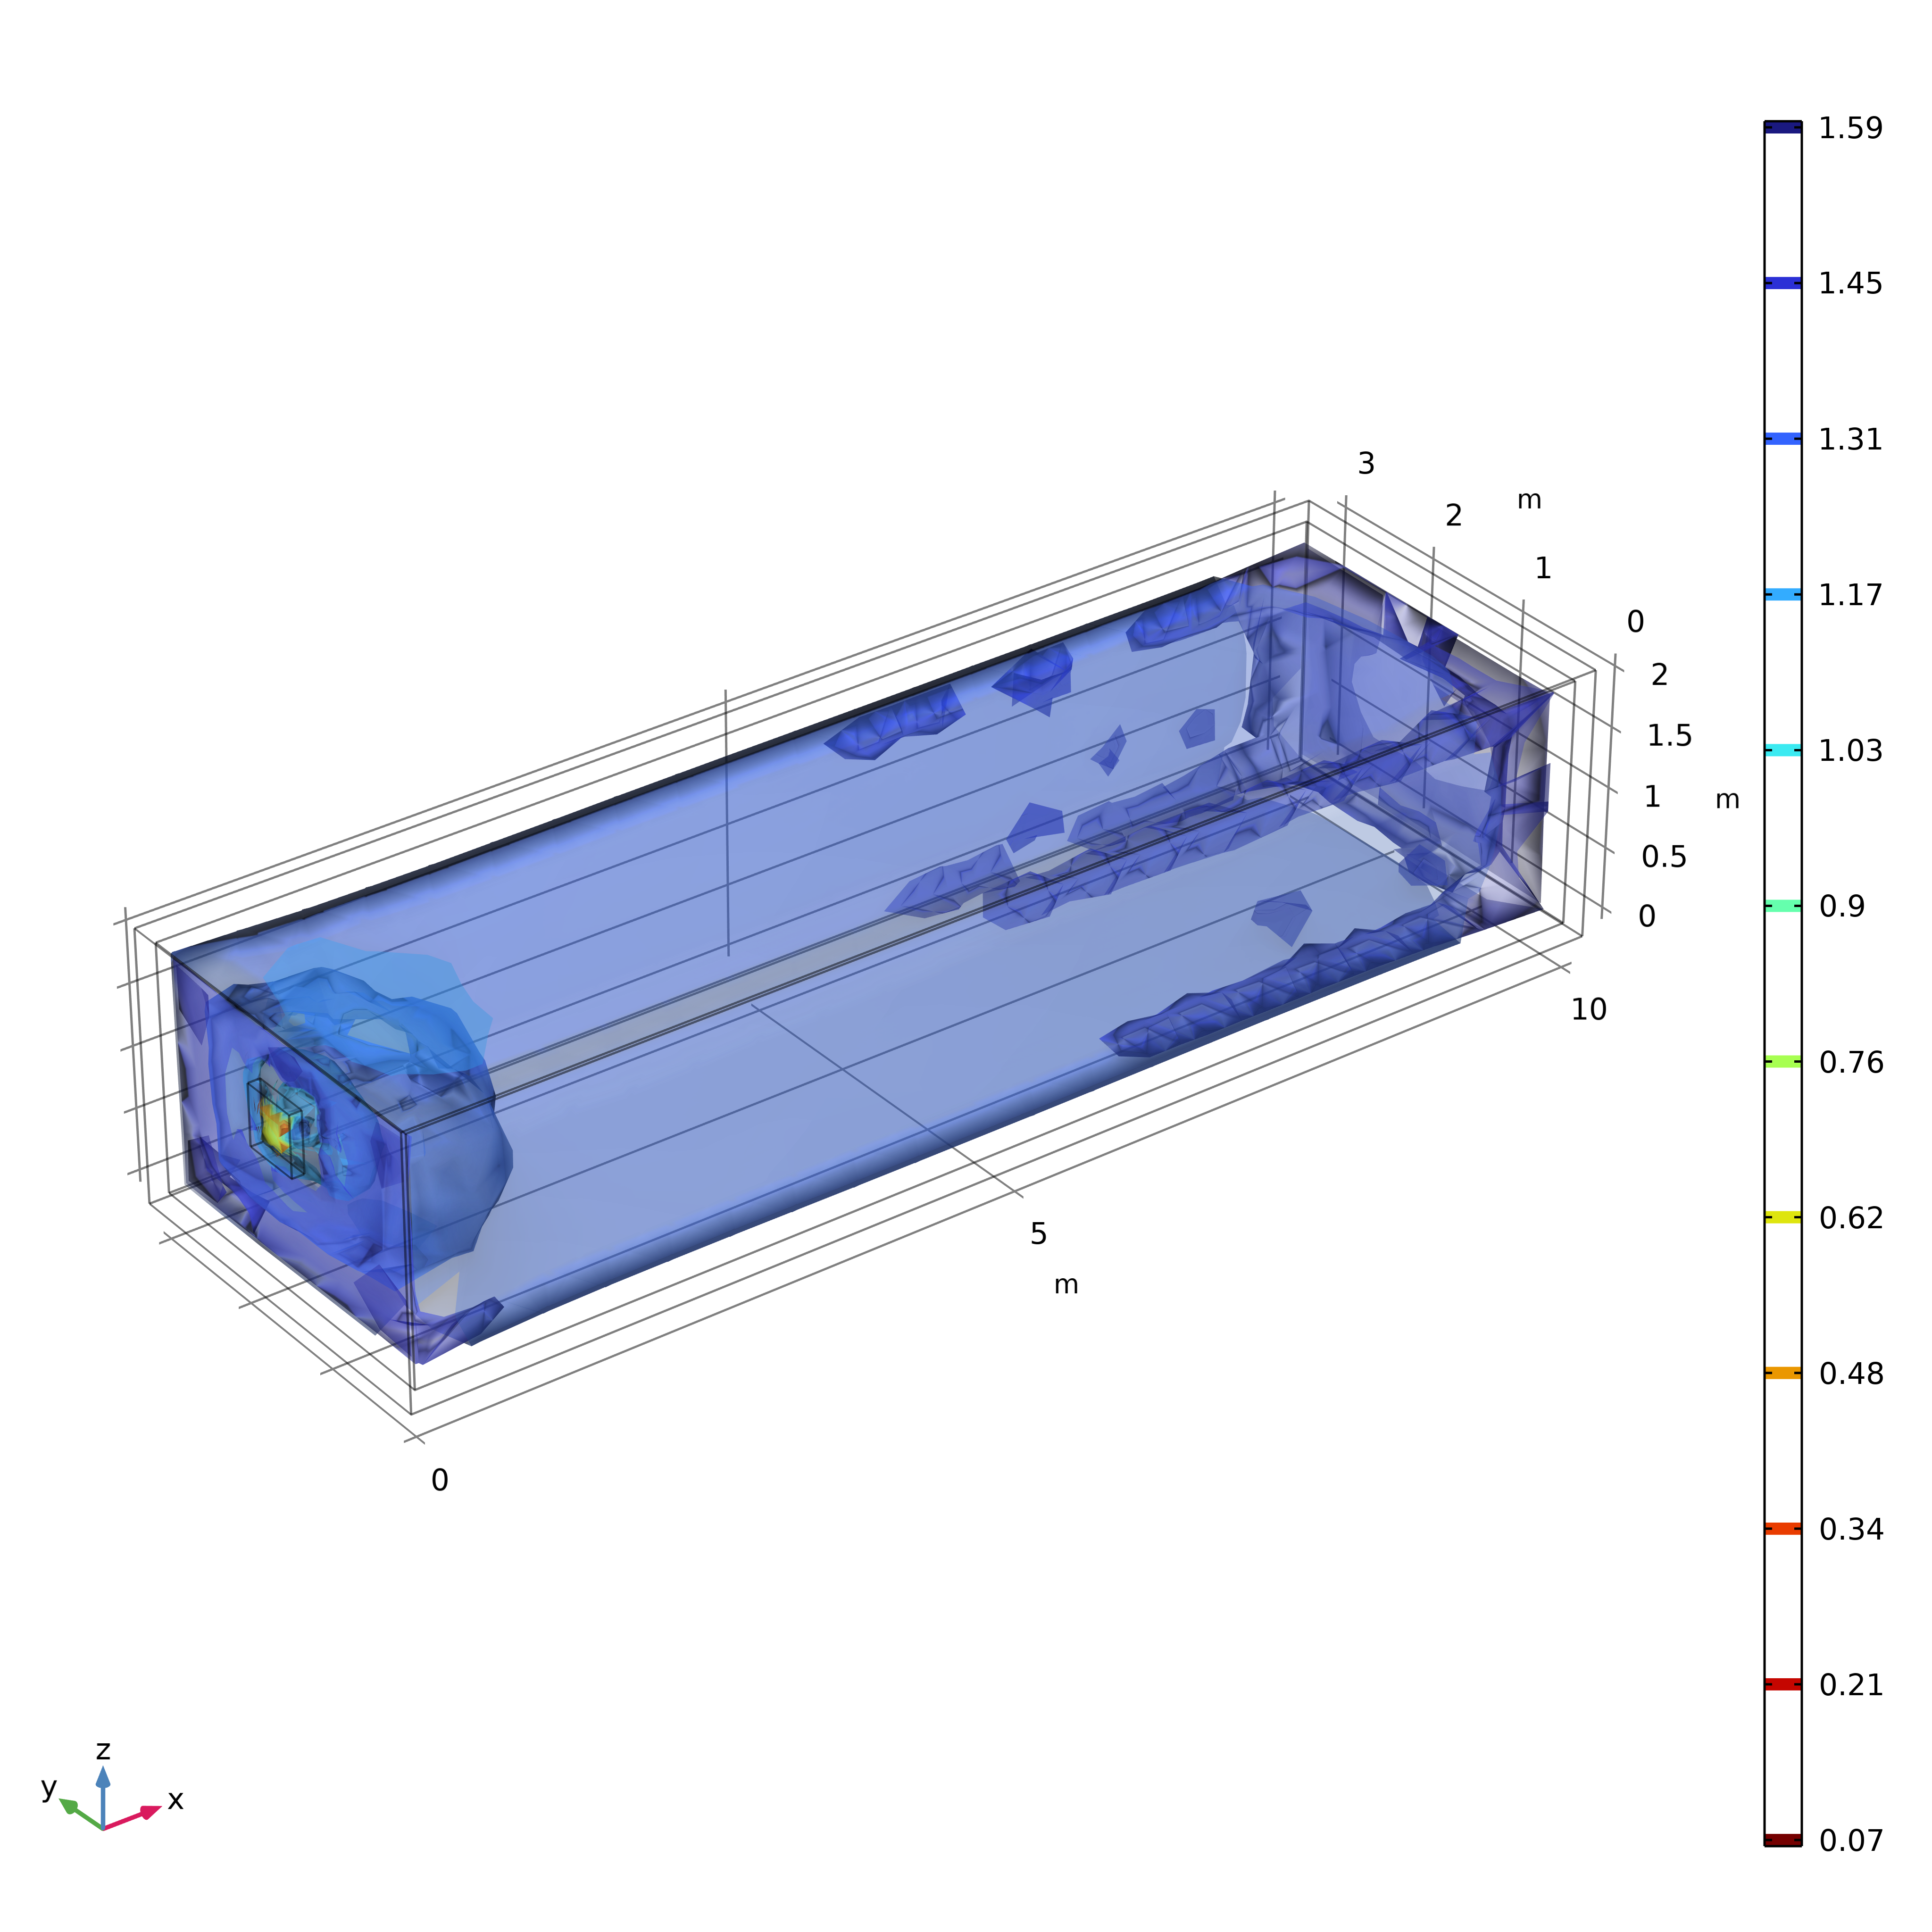
\includegraphics[width=0.4\textwidth]{figures/Crop-free glass greenhouse wind speed.png}
      }
       \caption{Plot for the Crop-Free Greenhouse}
       \label{Plot for the Crop-Free Greenhouse}
  \end{figure}

% 两张图片并列
\begin{figure}[htbp]
     
      \centering
      \subfigure[Temperature Distribution Plot at 0.5m Cross-Section of the Crop-Free Greenhouse] { 
          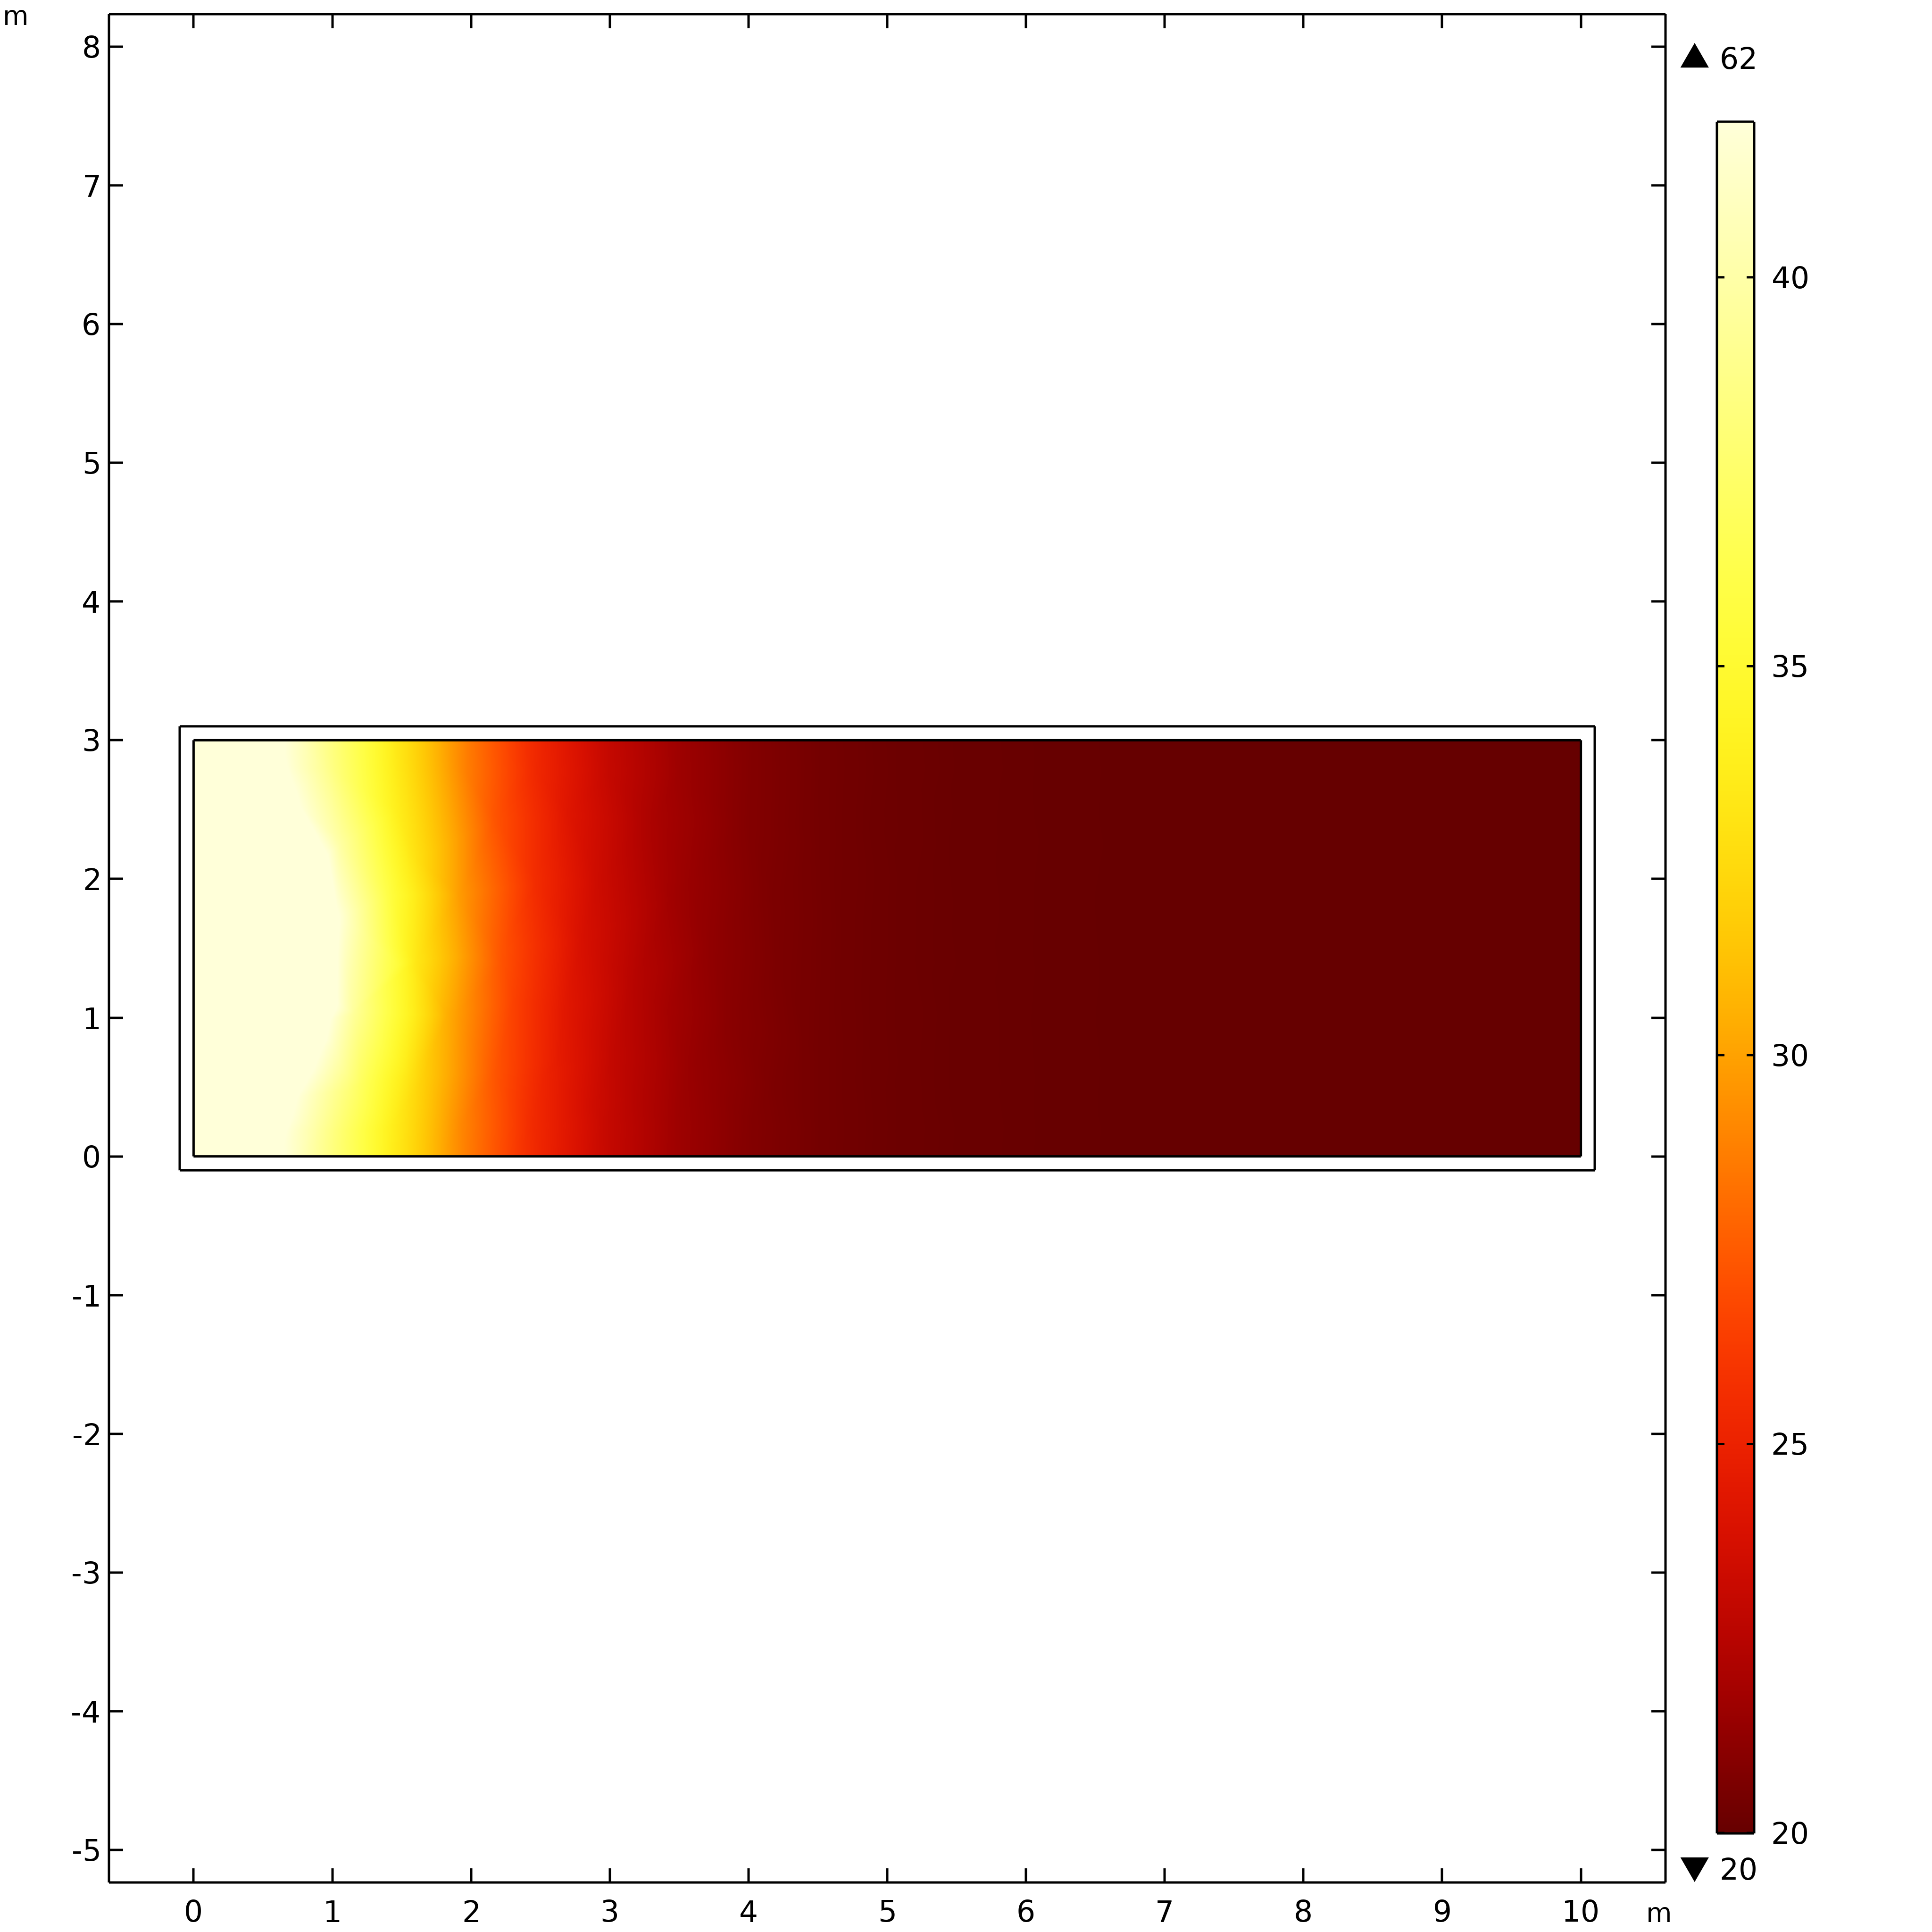
\includegraphics[width=0.4\textwidth]{figures/Temperature Distribution Plot at 05m Cross-Section of the Crop-Free Greenhouse.png}
          \label{Temperature Distribution Plot at 0.5m Cross-Section of the Crop-Free Greenhouse}
          
      }
       \subfigure[Wind Speed Distribution Plot at 0.5m Cross-Section of the Crop-Free Greenhouse] { 
         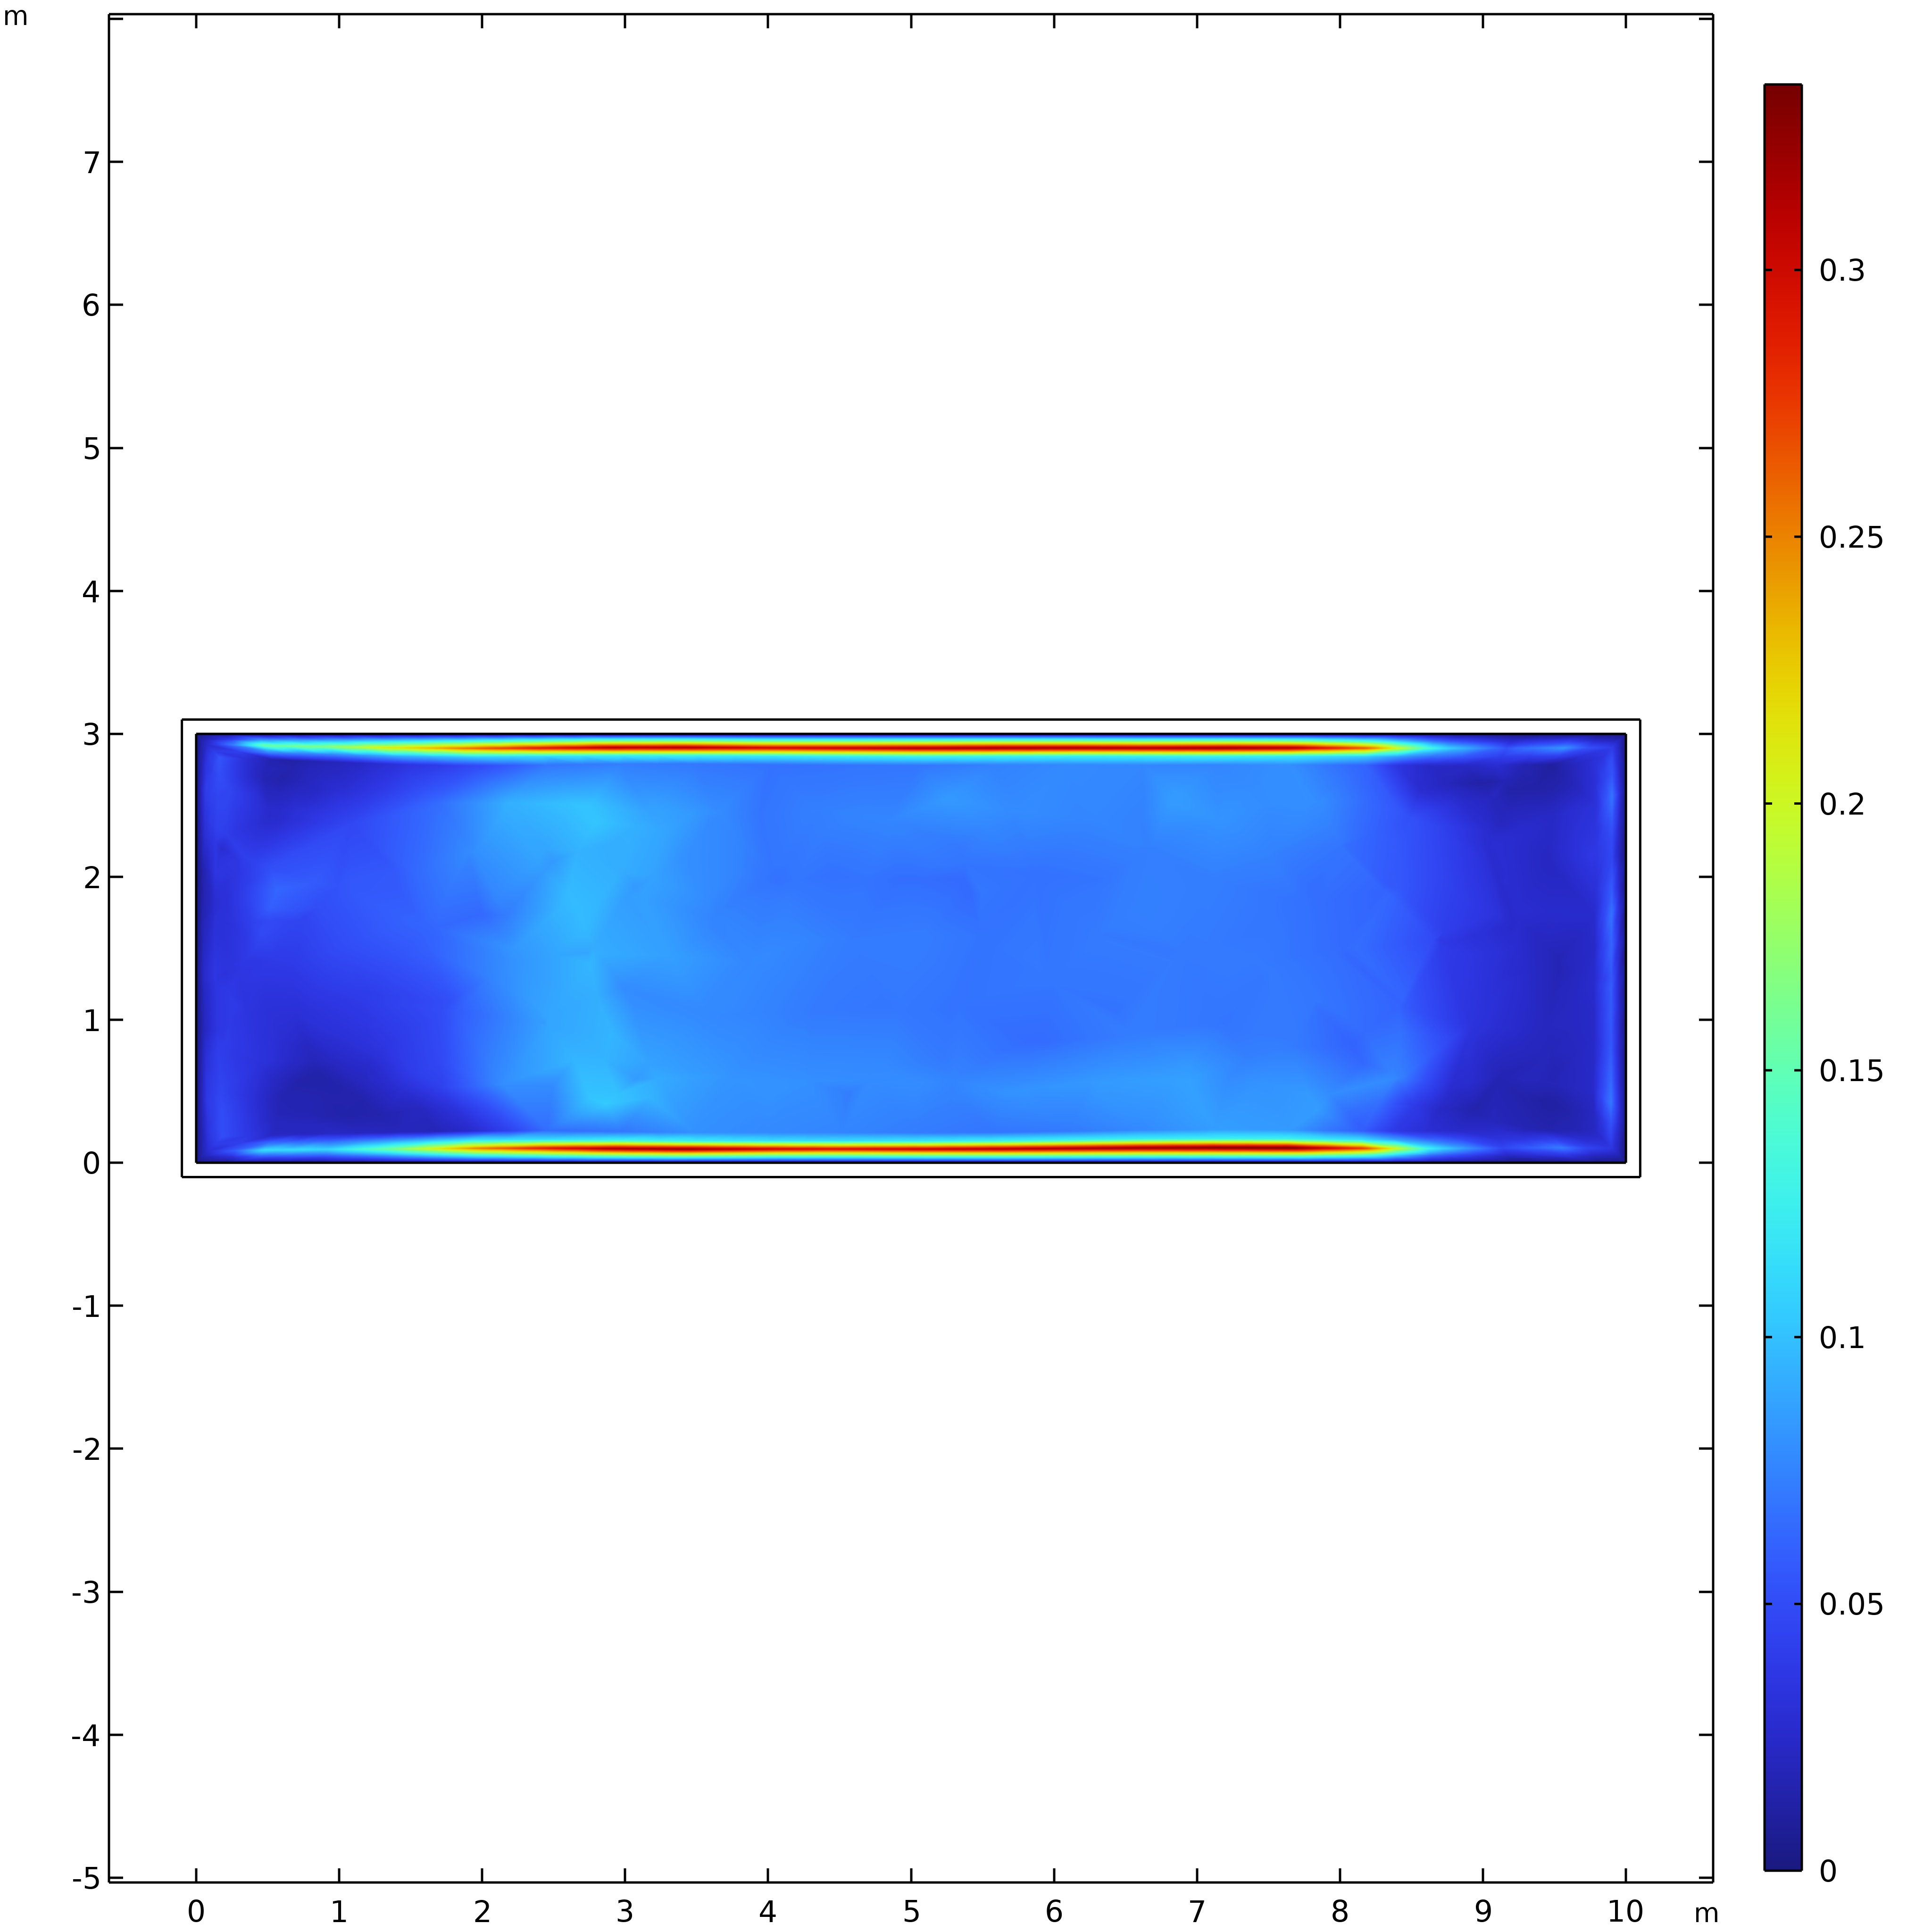
\includegraphics[width=0.4\textwidth]{figures/Wind Speed Distribution Plot at 05m Cross-Section of the Crop-Free Greenhouse.png}
         \label{Wind Speed Distribution Plot at 0.5m Cross-Section of the Crop-Free Greenhouse}
      }
       \caption{Plot at 0.5m Cross-Section of the Crop-Free Greenhouse}
        \label{Plot at 0.5m Cross-Section of the Crop-Free Greenhouse}
  \end{figure}


\subsubsection{Analysis of the Result}
% \begin{itemize}
% \item Local optimization and overall optimization:
% \item Sensitivity: The result is quite sensitive to the change of the three parameters
% \item
% \item Trend:
% \item Comparison:
% \end{itemize}

We simulated the crop-free glass greenhouse and calculated the temperature distribution for each hour from 1 to 24, as shown in Figure \ref{Temperature Distribution Plot at 0.5m Cross-Section of the Crop-Free Greenhouse}. It can be observed that the temperature near the greenhouse fan has risen to 40 degrees Celsius, while the temperature in areas farther from the fan remains around 21-23 degrees Celsius. From Figure \ref{Wind Speed Distribution Plot at 0.5m Cross-Section of the Crop-Free Greenhouse}, it can be seen that after ventilation, the wind speed in the middle of the greenhouse can reach 0.2m/s, while the wind speed on both sides is higher, reaching 0.3m/s.
% 我们对无作物玻璃温室进行模拟,并且计算出从1-24小时每个状态的结构,如图???可以看出靠近温室风机的温度已经上升到40摄氏度,距离风机较远地区温度保持在21-23度左右。从图可以看出通风后,温室中间风速可以达到0.2m/s,两侧风速较大,达到0.3m/s.

\subsection{Temperature and Wind Speed Distribution in a Glass Greenhouse with Crops}
%种植作物玻璃温室温度和风速分布

\subsubsection{Porous Medium Model}
%多孔介质模型

In greenhouse simulation, treating cultivated crops as a porous medium is an innovative approach that holds the potential to deepen our understanding of gas flow and plant influence within the greenhouse. Studies referenced in literature \cite{4} and \cite{6} involve establishing a mathematical model for the interaction between crops and greenhouse airflow using the Darcy-Forchheimer law. The Darcy-Forchheimer law provides a theoretical framework for describing gas or liquid flow in porous media.

We consider the crops themselves as a porous medium within the greenhouse, containing numerous small channels and gaps internally. These channels influence the characteristics of gas flow within the greenhouse, and the Darcy-Forchheimer law offers a quantitative way to describe this impact. 
% 在温室模拟中,将种植作物视为多孔介质是一种创新的方法,它有望深化我们对温室内气体流动和植物影响的理解。有关文献和的研究,涉及到使用Darcy-Forchheimer定律建立作物与温室气流速度之间的数学模型。Darcy-Forchheimer定律是描述多孔介质中气体或液体流动的理论框架。我们将作物本身看作温室内的多孔介质,其内部存在许多微小的通道和空隙。这些通道会影响温室内气体流动的特性,而Darcy-Forchheimer定律为我们提供了一个定量的方式来描述这种影响。

The movement of crops to fluids is mainly to create resistance and slow down the movement of fluids. The effect on the momentum of the control element is defined as $S_\varphi $, which is mathematically modeled according to the Darcy-Forchheimer law and added to the momentum equation as a source term:
%农作物对流体运动,主要是产生阻力减缓流体的运动。对控制元动量的影响定义为Sφ,根据Darcy-Forchheimer定律建立其与流体速度之间的数学模型,并作为源项添加到动量方程中:
$$ S_\varphi =-\left ( \frac{\mu }{K_p} +\tfrac{C_F}{\sqrt{K_p} } \rho u^2  \right ) $$

$S_\varphi $ is the momentum source term; $K_p$ is the permeability coefficient of the porous medium; $C_F$ is the nonlinear momentum loss coefficient; $\mu$ is the dynamic viscosity of air; $\rho$ is the density of the air; $u$ is the air velocity.
% S是动量源项;Kp是多孔介质的渗透性系数;CF是非线性动量损失系数;μ是空气的动力黏度;ρ是空气的密度;u是空气流速。

This law considers nonlinear effects arising from the medium's structure, which is crucial for simulating gas flow under actual greenhouse conditions. We can incorporate factors such as porosity within the crops, stomatal distribution, and crop density into the model to more accurately reflect the complex gas flow within the greenhouse.
%通过将Darcy-Forchheimer定律引入数学模型,我们可以考虑到作物的多孔性对气流速度的影响。该定律考虑了由于介质结构引起的非线性效应,这对于模拟实际温室条件下的气体流动至关重要。我们可以将作物内部的孔隙度、气孔分布以及作物密度等因素纳入模型,以更准确地反映出温室内部的复杂气体流动情况。

According to the research, $S_\varphi $ can be correlated with the leaf density, resistance coefficient, and other related exponents of plants, and these parameters can be used to directly establish the relationship with $u^2$, the specific form is as follows
%根据研究,Sφ又可以和植物叶子密度,阻力系数等相关的指数相关,利用这些参数直接建立和u2的关系,具体形式如下:

   $$S_\varphi =-I_{LAV}C_D\rho u^2$$
where $I_{LAV}$ is the leaf area index; $C_D$ is the drag coefficient of the crop canopy. Due to the slow flow of gas, the dynamic viscosity is very small, and the first term of $S_\varphi$ can be ignored, so as to obtain the formula for calculating $\frac{C_F}{\sqrt{K_p}}$:
   %其中,ILAV是叶面积指数;CD是作物冠层的阻力系数。由于气体流动的比较慢,动力黏度很小,可以忽略Sφ的第一项,从而得到$\frac{C_F}{\sqrt{K_p}$计算公式:

   $$\frac{C_F}{\sqrt{K_p} } =I_{LAP}C_D$$
By looking up, we get the parameters $C_D$=0.32,$I_{CA}$=3.0.
   %通过查阅,我们得到参数CD=0.32,ICA=3.0.
We get the final momentum equation:
   %我们得到最后的动量方程:
   $$\begin{equation}
\rho \left(\frac{\partial \mathbf{v}}{\partial t} + \mathbf{v} \cdot \nabla \mathbf{v}\right) = -\nabla p + \mu \nabla^2 \mathbf{v} - I_{LAP}C_D \rho u^2 
\end{equation}$$
   %对于作物呼吸作用以及和环境交换热的效应并不是研究重点,不予以考虑。
\subsubsection{Simulation of a Glass Greenhouse with Cultivated Crops}
% 种植作物玻璃温室仿真

Building upon the previous geometric model of the crop-free glass greenhouse, we have incorporated a crop model. The specific model is illustrated in Figure \ref{Geometric model diagram}. With the geometric model established, we have introduced crops as a porous medium. The simulation results were obtained through calculations based on this modified model.
% 基于之前的无作物玻璃温室几何模型,我们加入了作物模型,具体模型如图,建立好几何模型,我们在原来基础上把作物设置为多孔介质,进行计算得出仿真结果。

\subsubsection*{The simulation results for ventilation at 1.3m with a wind speed of 2m/s}
% 通风口位于1.3m,通风2m/s的仿真结果

% 温度图
\begin{figure}[htbp]
      \centering
      \subfigure[0.5m Cross-Section of the Glass Greenhouse] { 
          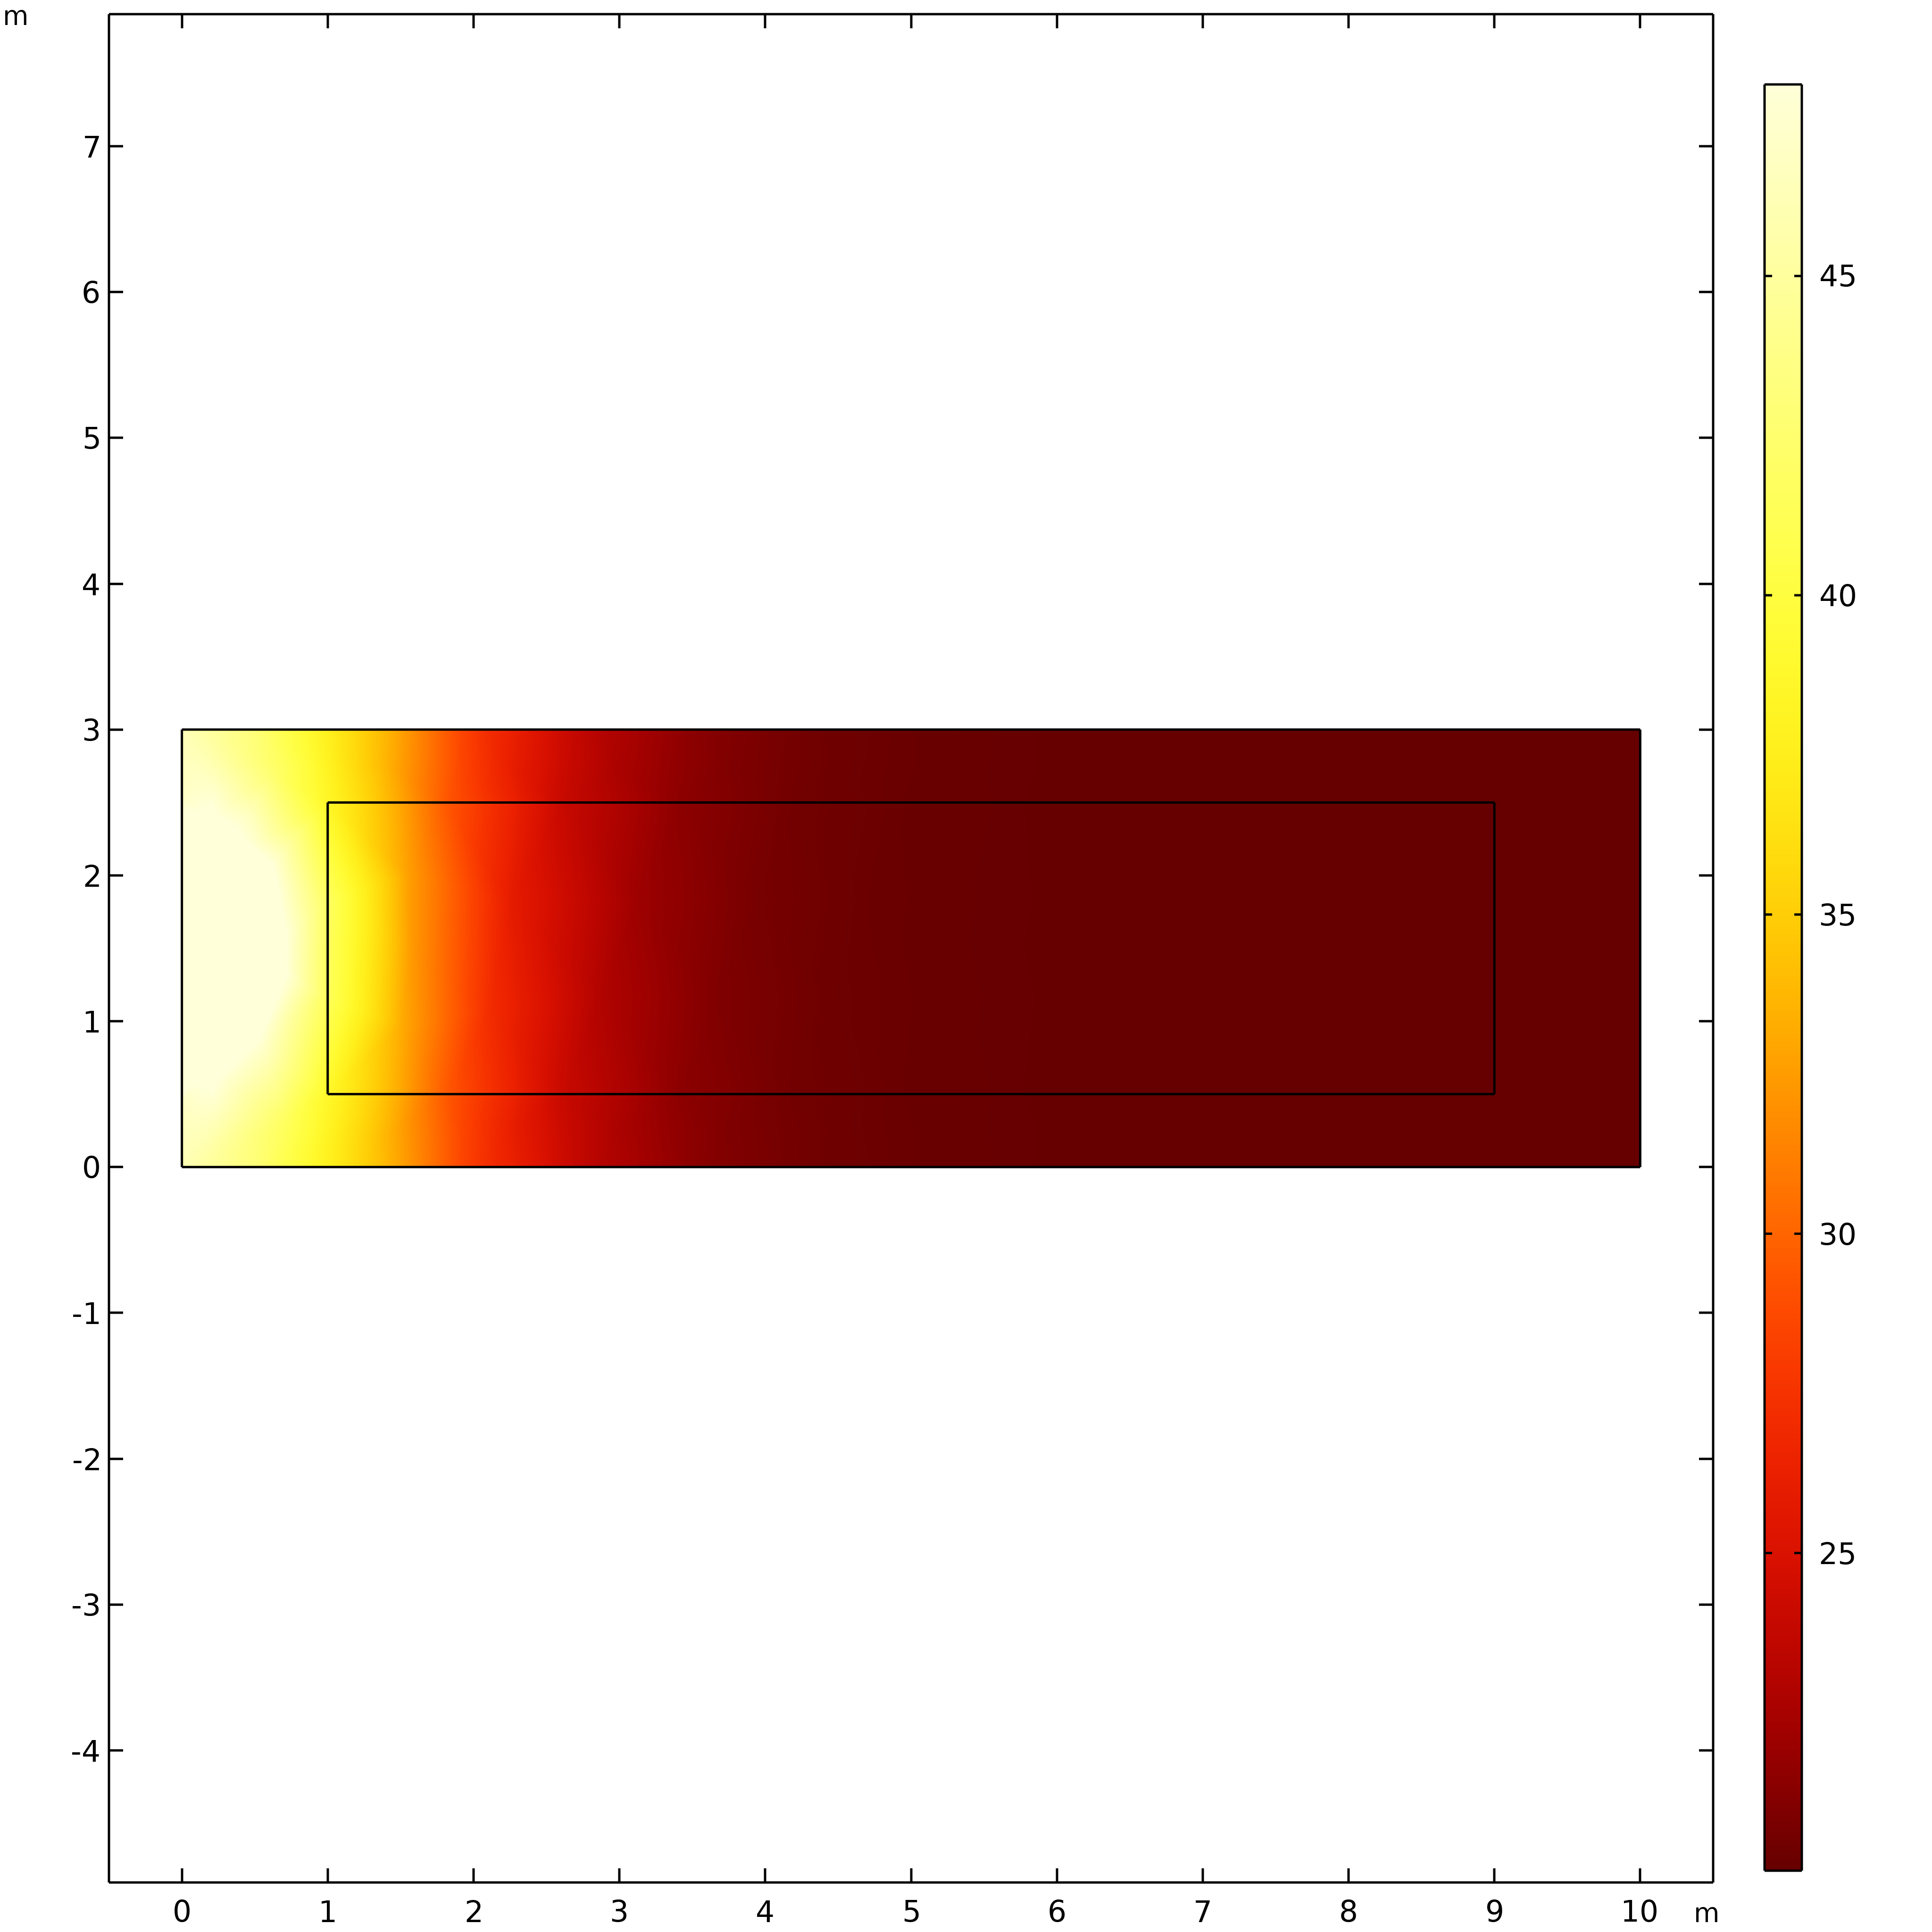
\includegraphics[width=0.4\textwidth]{figures/Temperature Distribution Plot at 05m Cross-Section of the Crop Greenhouse.png}
          \label{Temperature Distribution Plot at 0.5m Cross-Section of the Glass Greenhouse with Cultivated Crops}
          
      }
       \subfigure[0.1m Cross-Section of the Glass Greenhouse] { 
         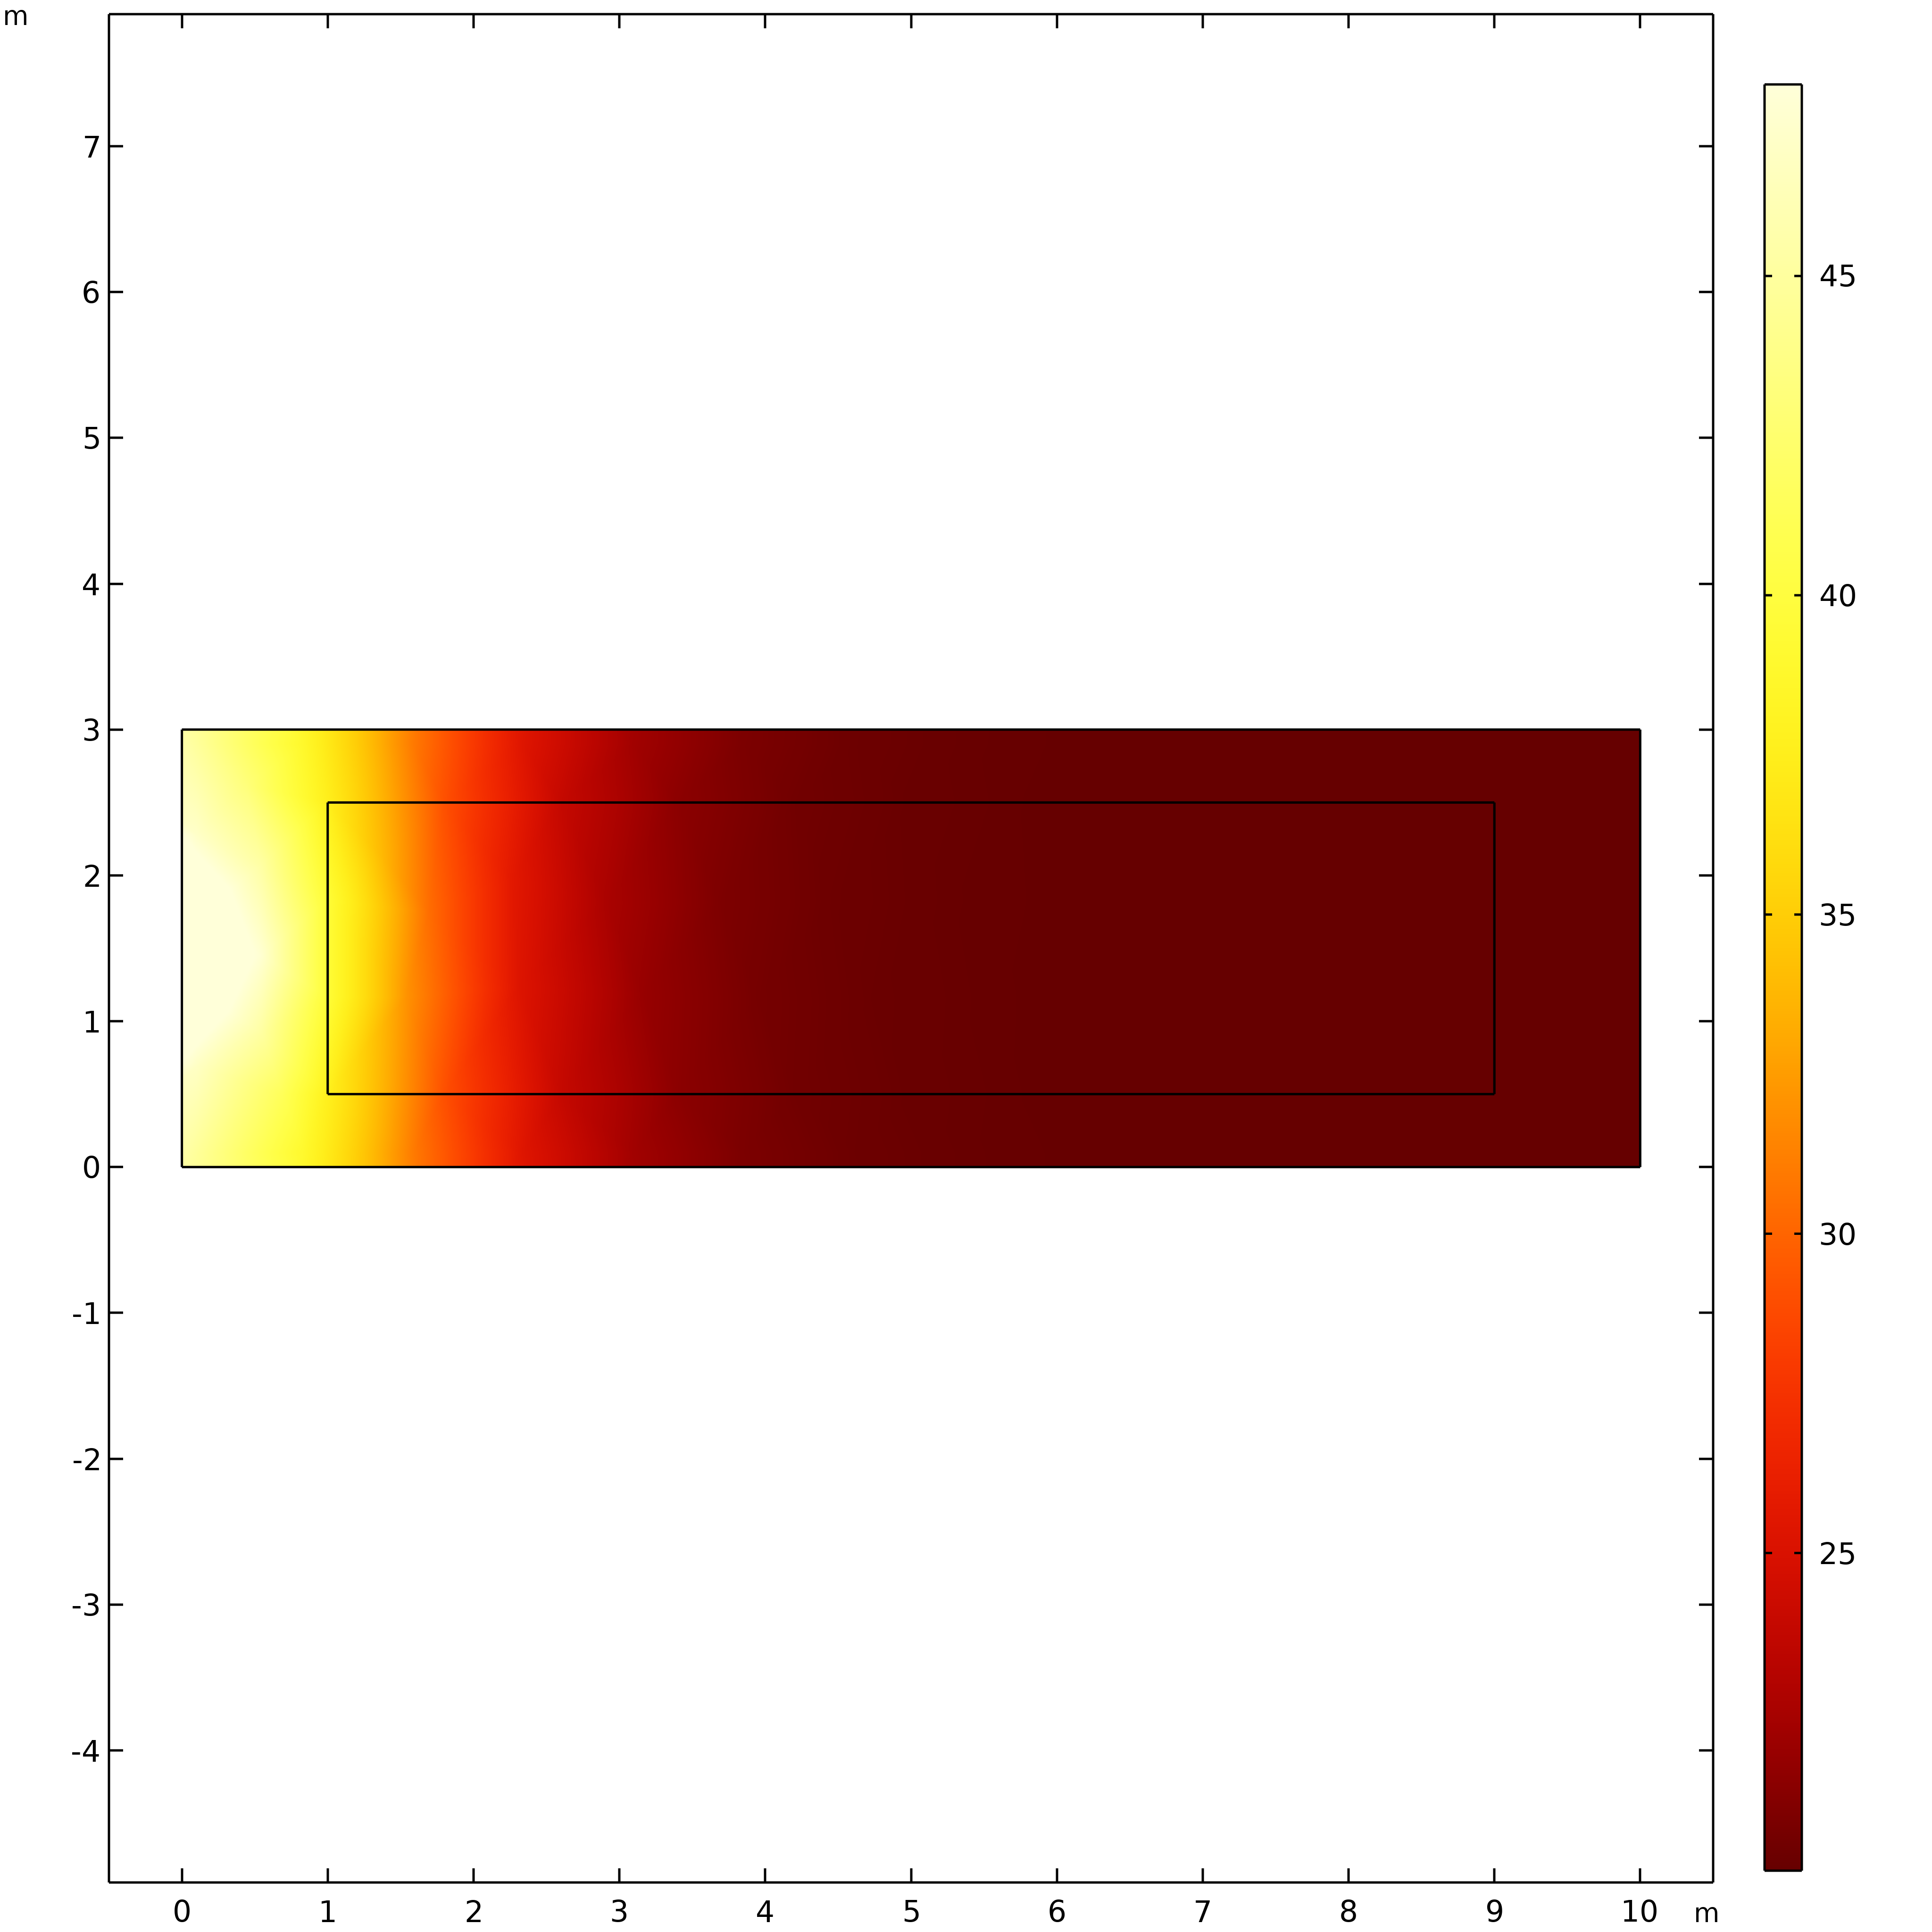
\includegraphics[width=0.4\textwidth]{figures/Temperature Distribution Plot at 01m Cross-Section of the Crop Greenhouse.png}
         \label{Temperature Distribution Plot at 0.1m Cross-Section of the Glass Greenhouse with Cultivated Crops}
      }
       \caption{Temperature Distribution Plot at the Glass Greenhouse with Cultivated Crops}
        \label{Temperature Distribution Plot at Cross-Section of the Glass Greenhouse with Cultivated Crops}
  \end{figure}

% 风速图
\begin{figure}[htbp]
      \centering
      \subfigure[0.5m Cross-Section of the Glass Greenhouse] { 
          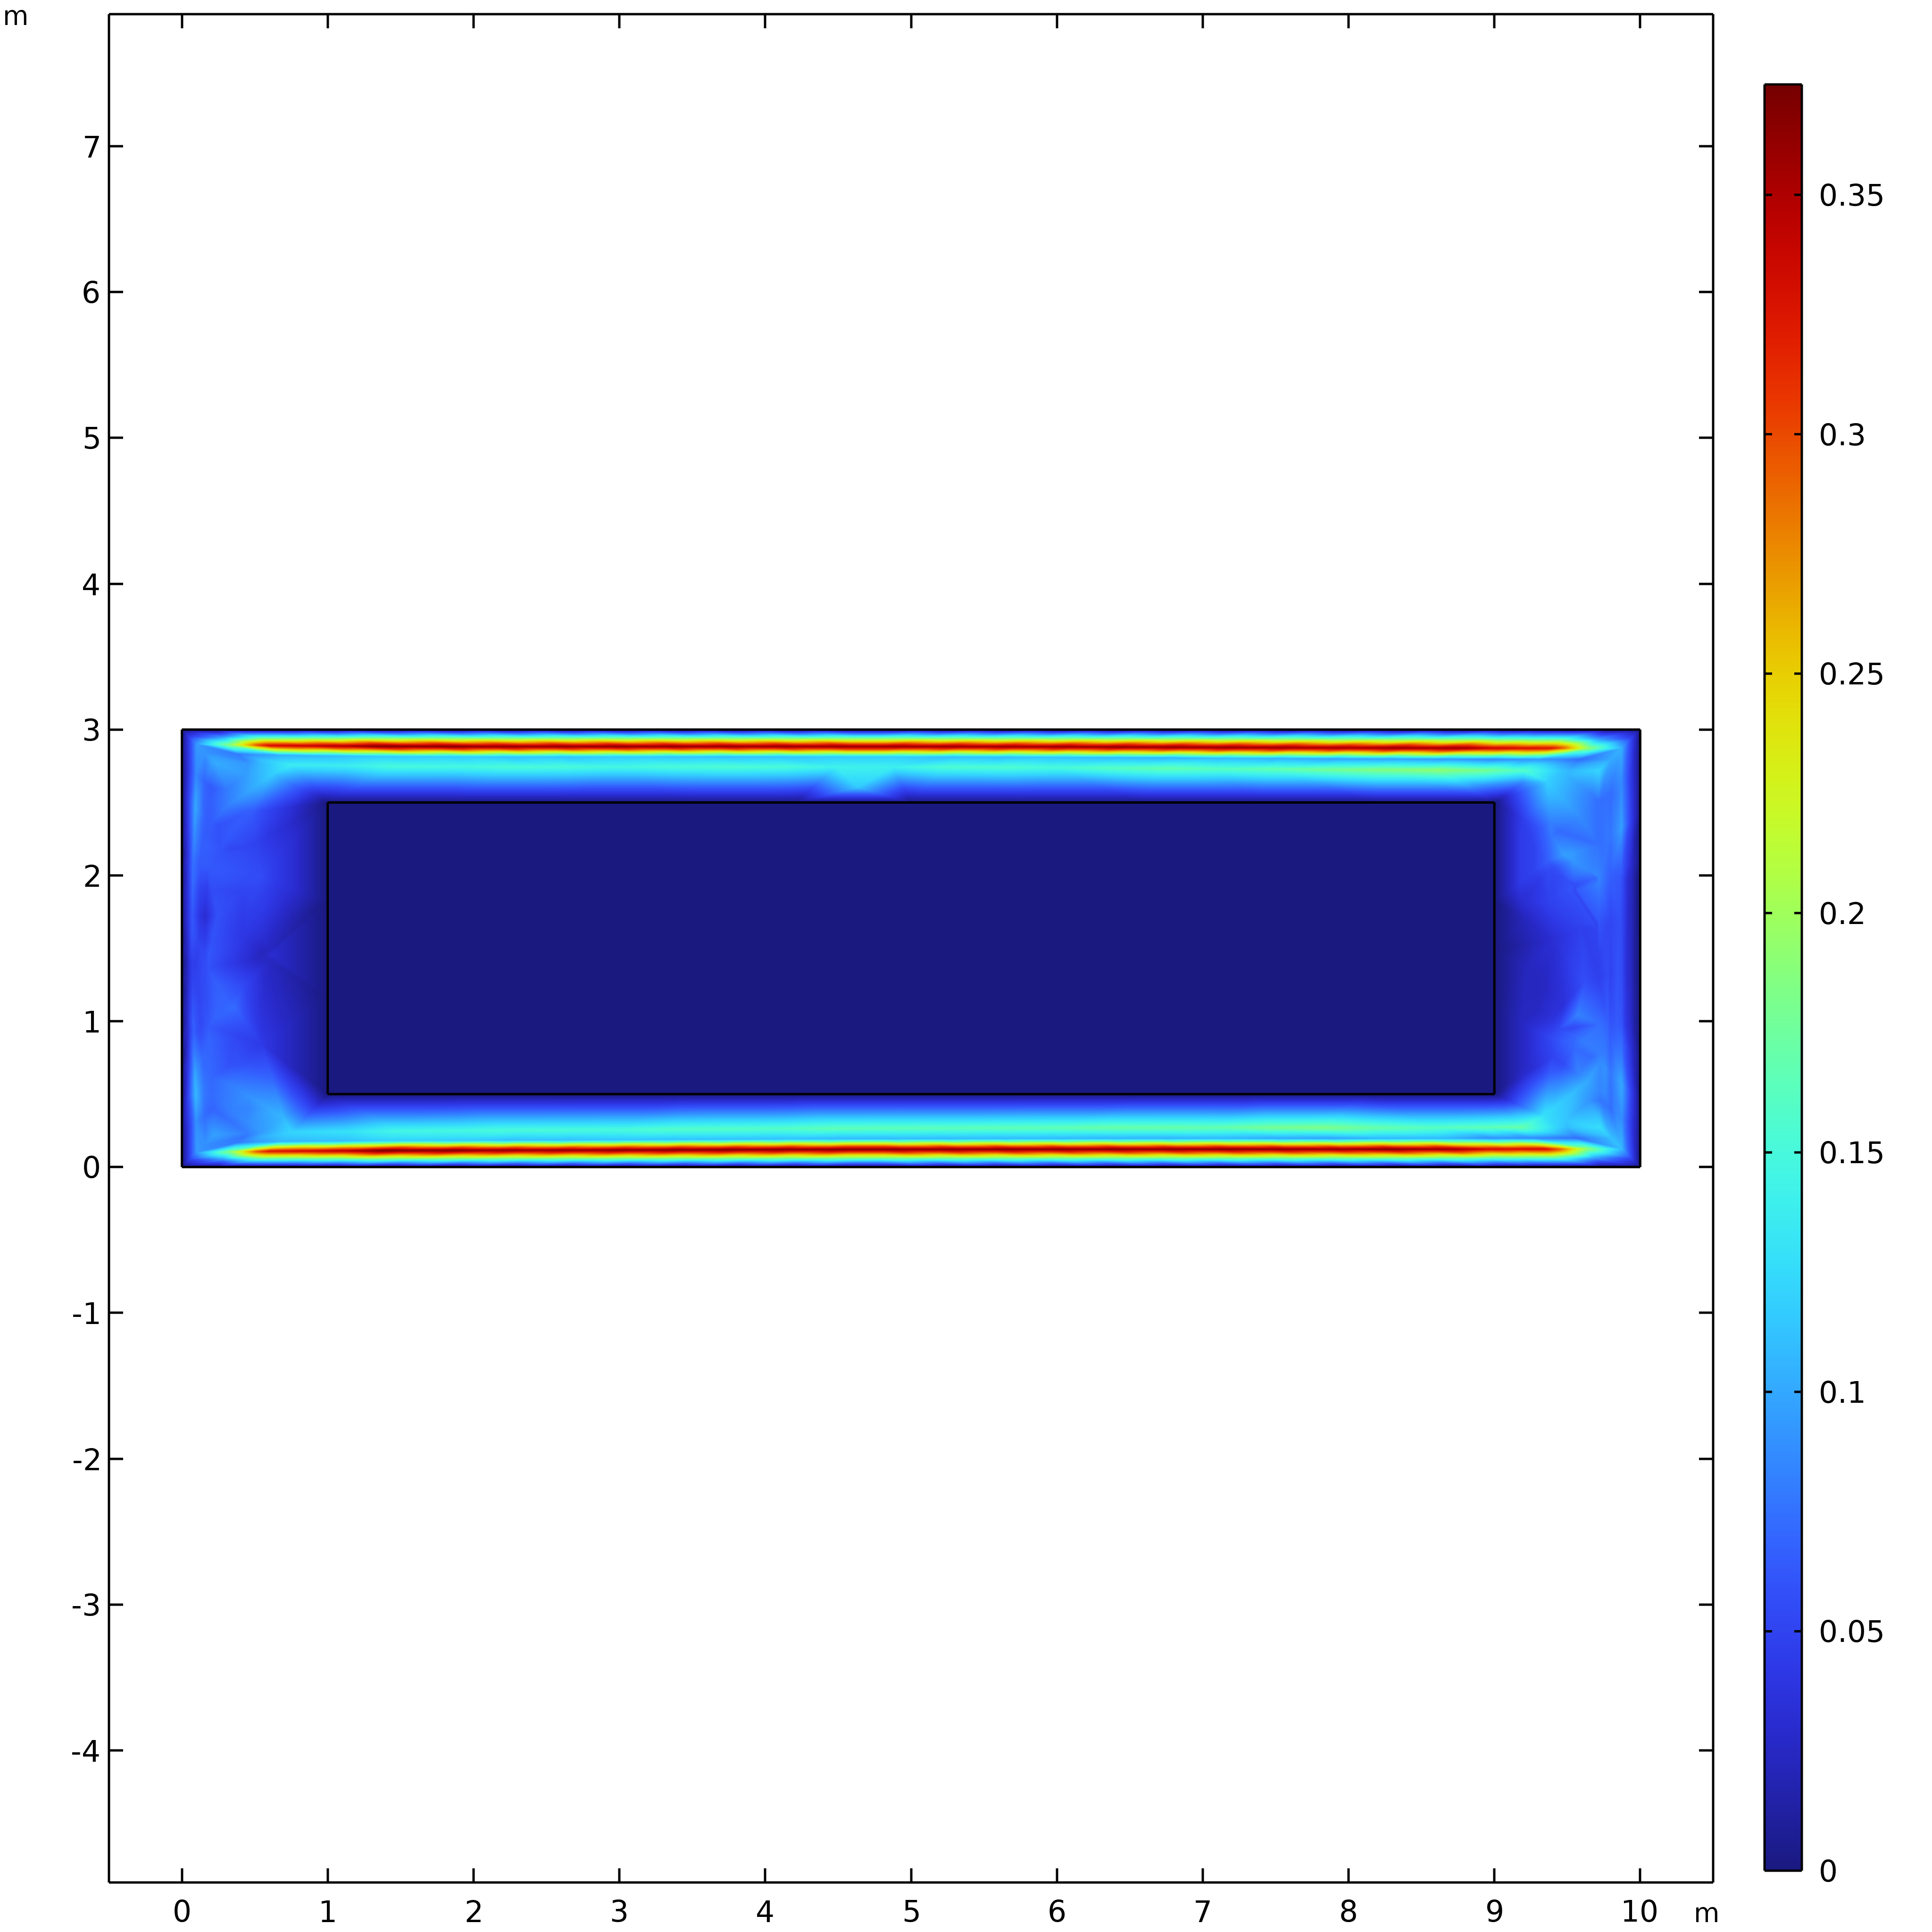
\includegraphics[width=0.4\textwidth]{figures/Wind Speed Distribution Plot at 05m Cross-Section of the Crop Greenhouse.png}
          \label{Wind Speed Distribution Plot at 0.5m Cross-Section of the Glass Greenhouse with Cultivated Crops}
          
      }
       \subfigure[0.1m Cross-Section of the Glass Greenhouse] { 
         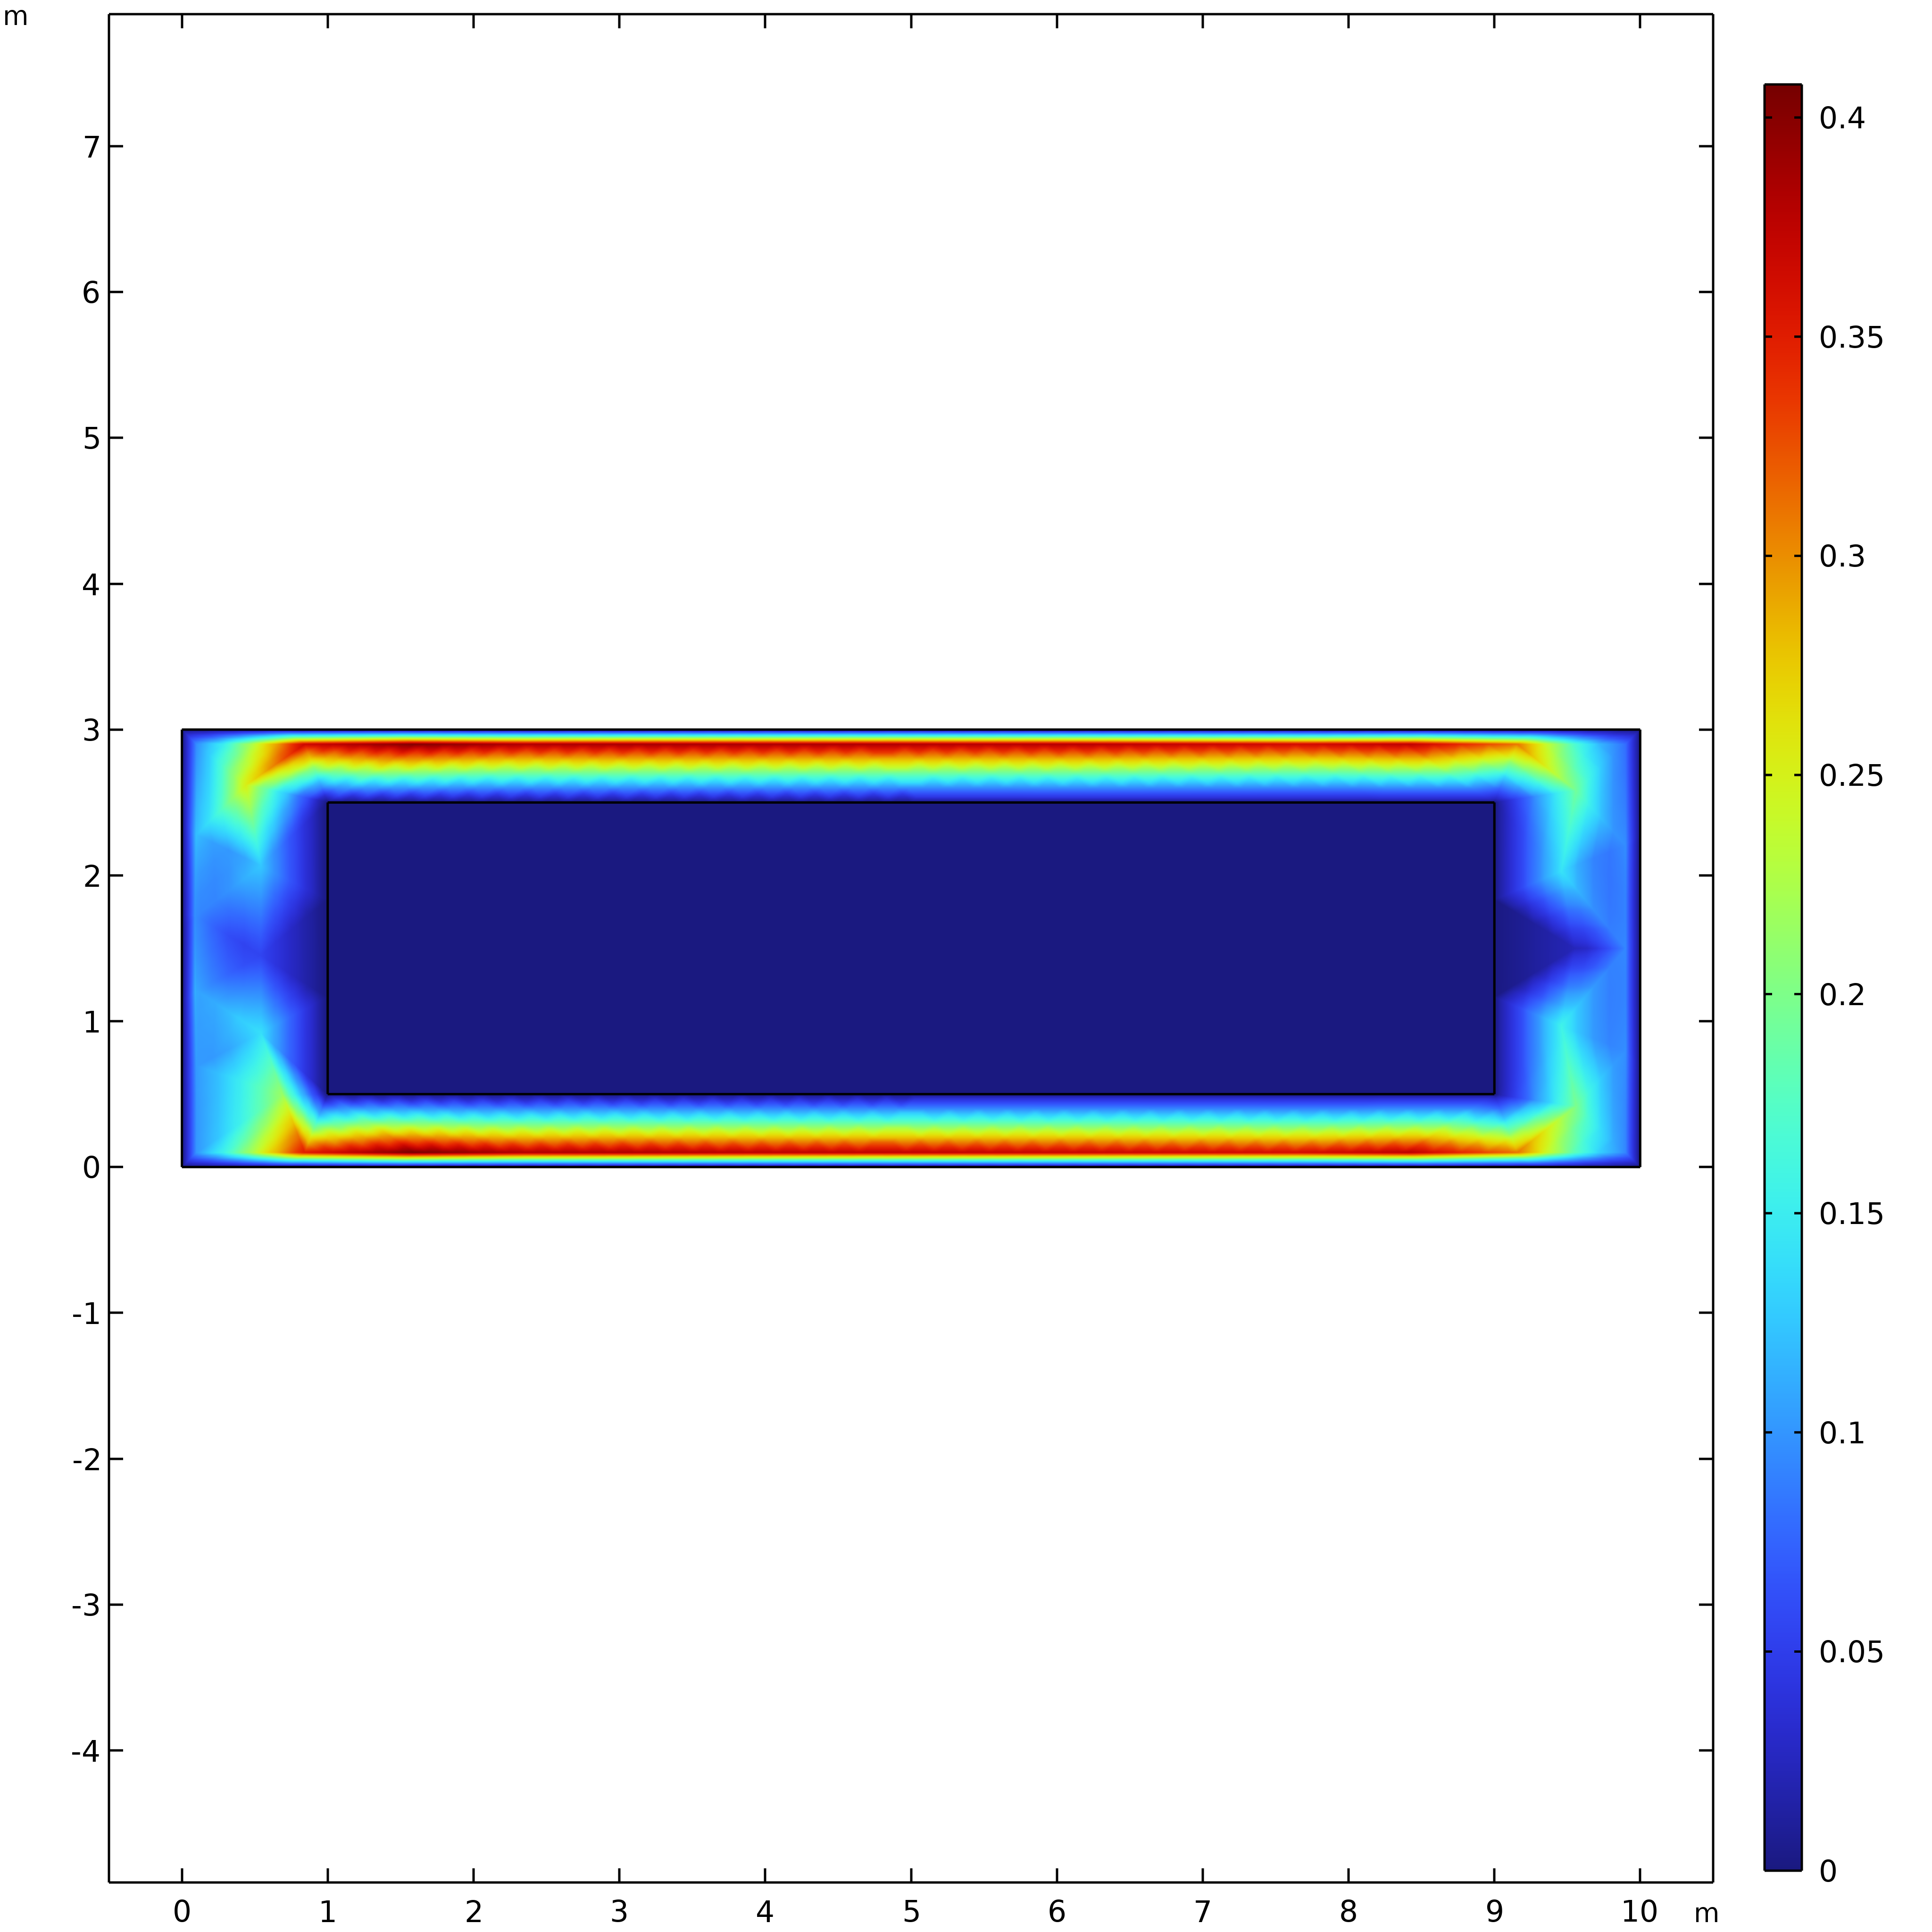
\includegraphics[width=0.4\textwidth]{figures/Wind Speed Distribution Plot at 01m Cross-Section of the Crop Greenhouse.png}
         \label{Wind Speed Distribution Plot at 0.1m Cross-Section of the Glass Greenhouse with Cultivated Crops}
      }
       \caption{Wind Speed Distribution Plot at the Glass Greenhouse with Cultivated Crops}
        \label{Wind Speed Distribution Plot at Cross-Section of the Glass Greenhouse with Cultivated Crops}
  \end{figure}
  
% 以下数据全是编的,我只求合理即可!!!!
Combining the temperature distribution plot in Figure \ref{Temperature Distribution Plot at Cross-Section of the Glass Greenhouse with Cultivated Crops}, it can be observed that temperatures near the warm air inlet at the 0.5 and 0.1 cross-sections are elevated, with some areas reaching 40 degrees. Approximately 75\% or more of the area is conducive to plant growth. Considering Figure \ref{Wind Speed Distribution Plot at Cross-Section of the Glass Greenhouse with Cultivated Crops}, the average air velocity at 0.5m above the ground, 0.21m/s, is below the optimal wind speed of 0.31m/s. The canopy portion of the plants is not in the most favorable wind speed range. At 0.1m above the ground, the average airflow velocity is 0.24m/s, also below the optimal wind speed. In conclusion, under these conditions, the temperature is suitable, but the wind speed is relatively slow, making it less ideal for plant growth.

% 结合下图\ref{Temperature Distribution Plot at Cross-Section of the Glass Greenhouse with Cultivated Crops},可以看出在0.5与0.1截面靠近暖风口的温度偏高,部分地区气温已经到达40度,大约有75%以上地区是有利于植物生长的。结合图\ref{Wind Speed Distribution Plot at Cross-Section of the Glass Greenhouse with Cultivated Crops},在距离地面 0.5 m 处的平均空气流速0.21m/s低于0.31m/s的最佳风速,植物冠层部分没有处于最适风速区域。在距离地面0.1 m 处气流平均流速为0.24m/s也低于最佳风速,总而言之该条件下温度合适,风速偏慢,不是很适合植物生长。


\subsubsection*{The simulation results for ventilation at 1.3m with a wind speed of 3m/s}
% 通风口位于1.3m,通风3m/s的仿真结果
% 温度图
\begin{figure}[htbp]
      \centering
      \subfigure[0.5m Cross-Section of the Glass Greenhouse] { 
          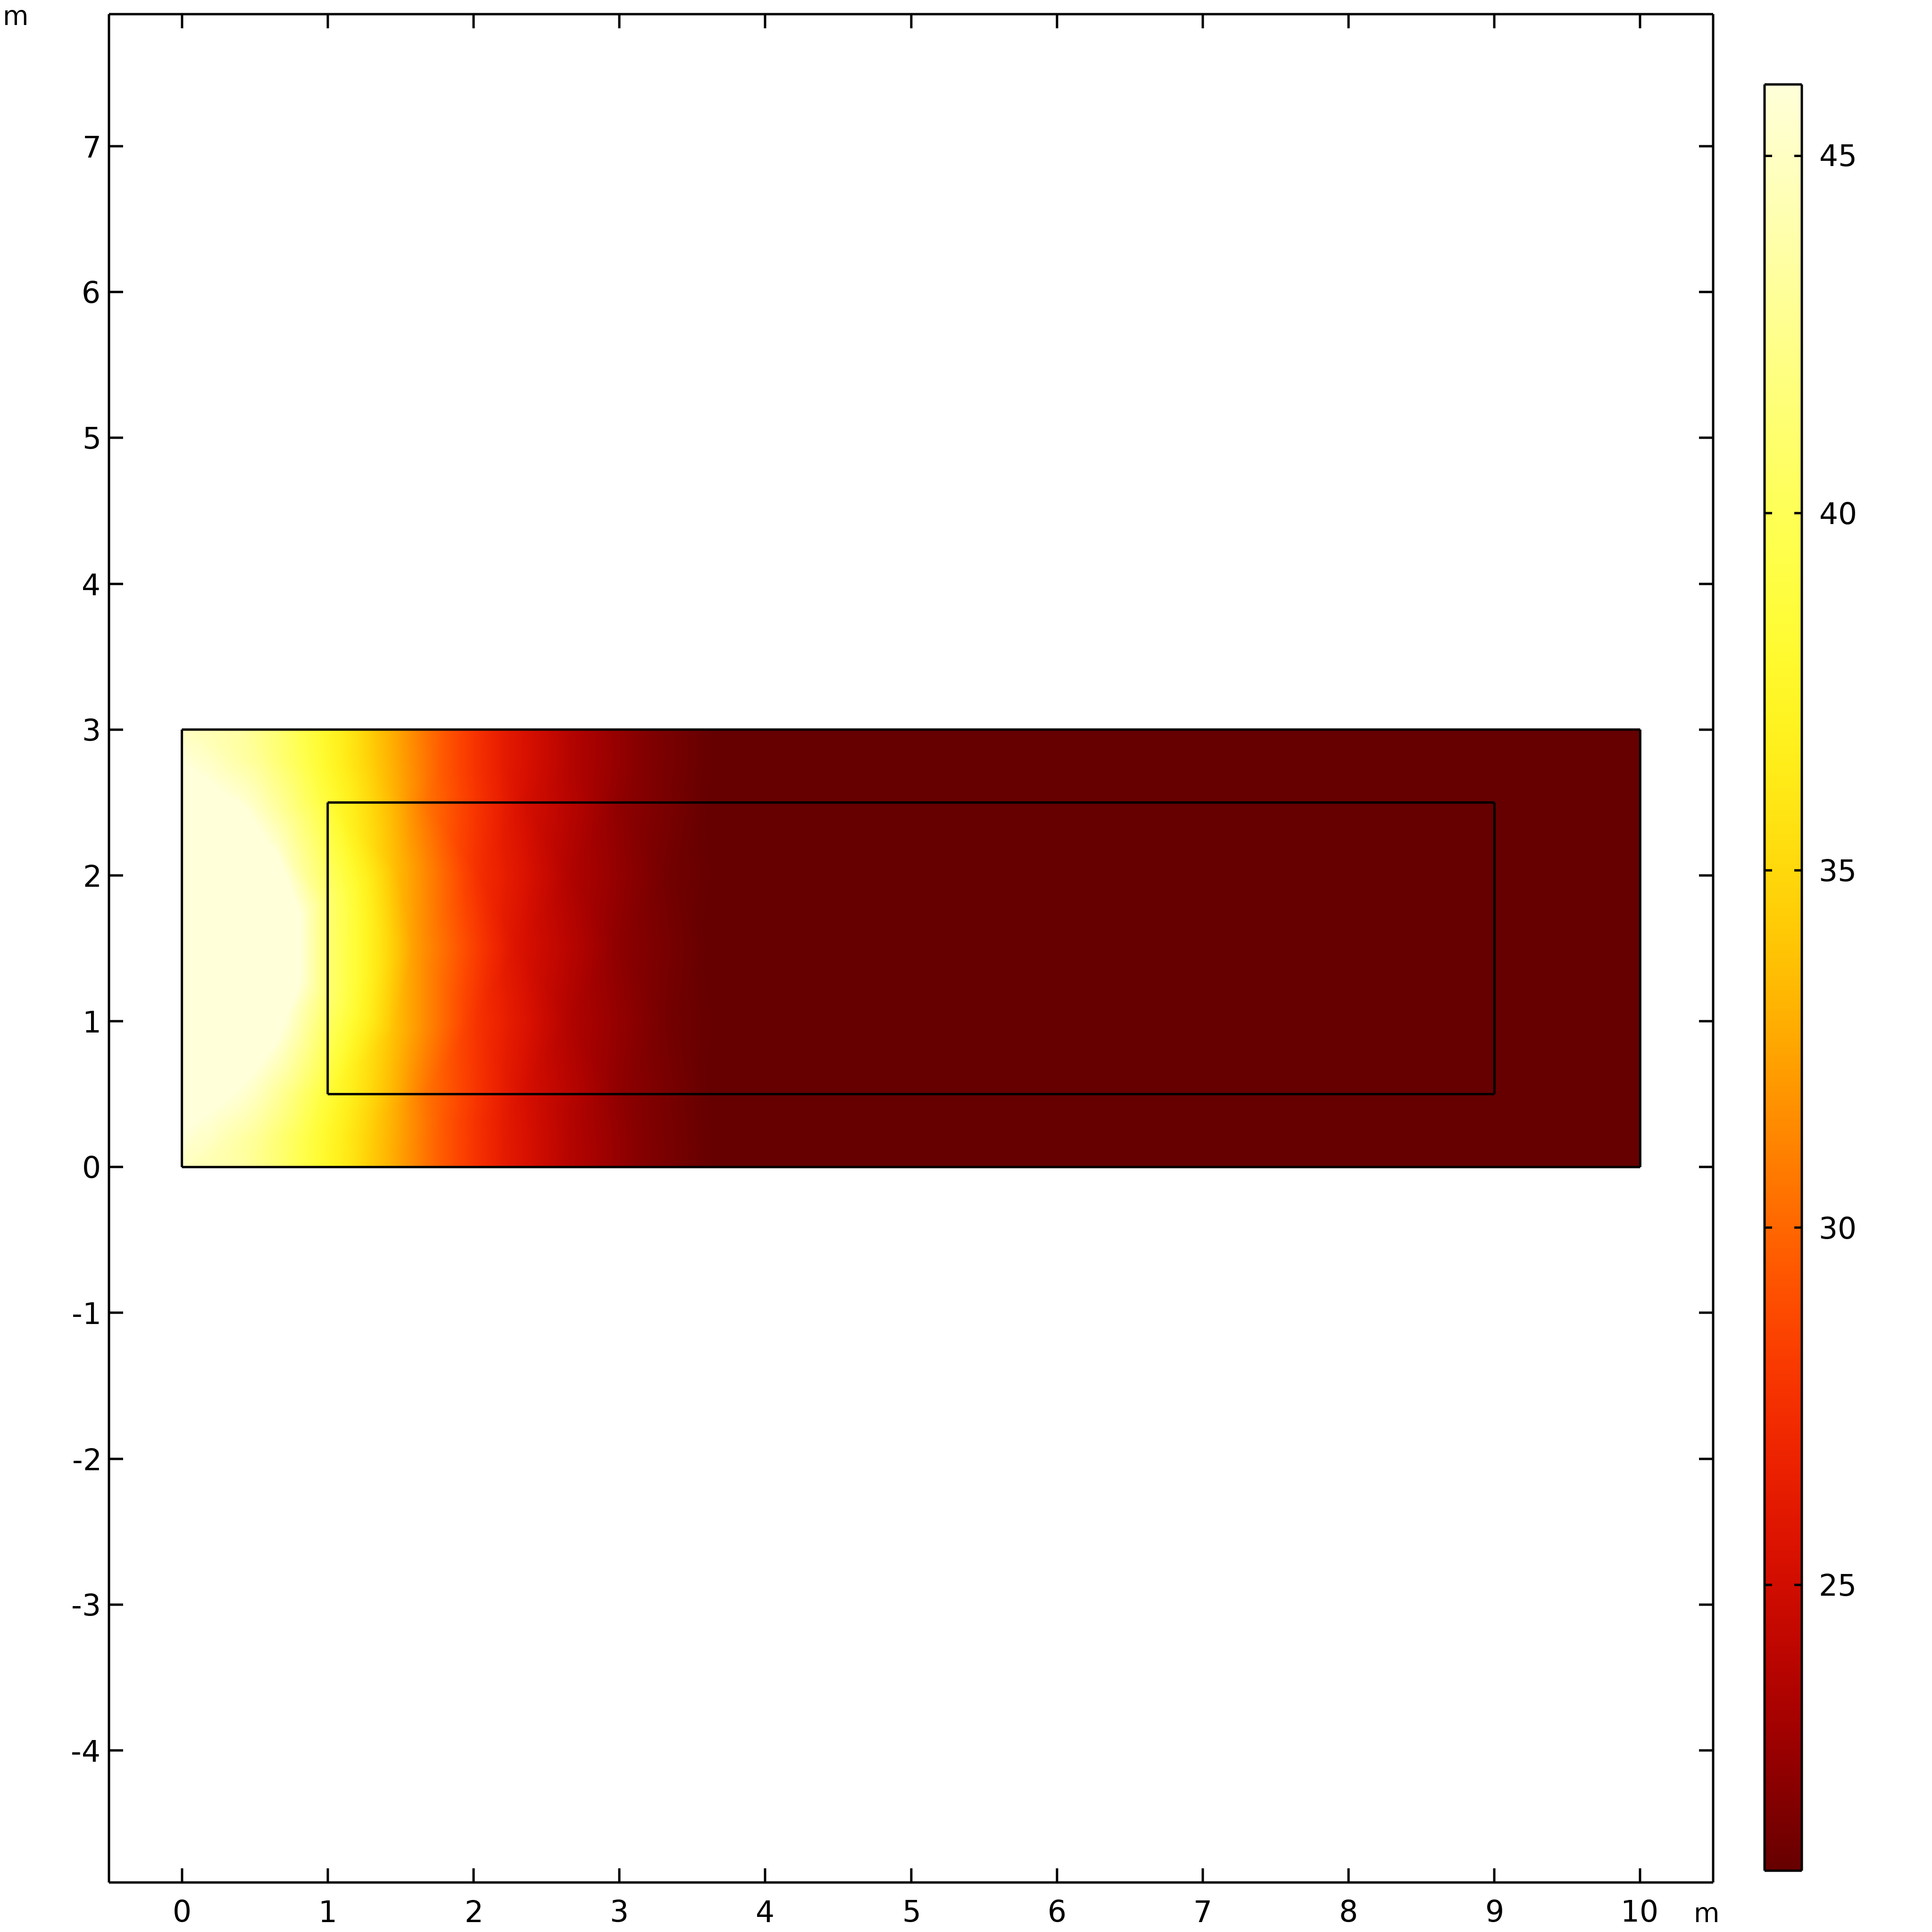
\includegraphics[width=0.4\textwidth]{figures/Temperature Distribution Plot at 05m Cross-Section of the Crop Greenhouse2.png}
          \label{Temperature Distribution Plot at 0.5m Cross-Section of the Glass Greenhouse with Cultivated Crops at a Wind Speed of 3m/s}
          
      }
       \subfigure[0.1m Cross-Section of the Glass Greenhouse] { 
         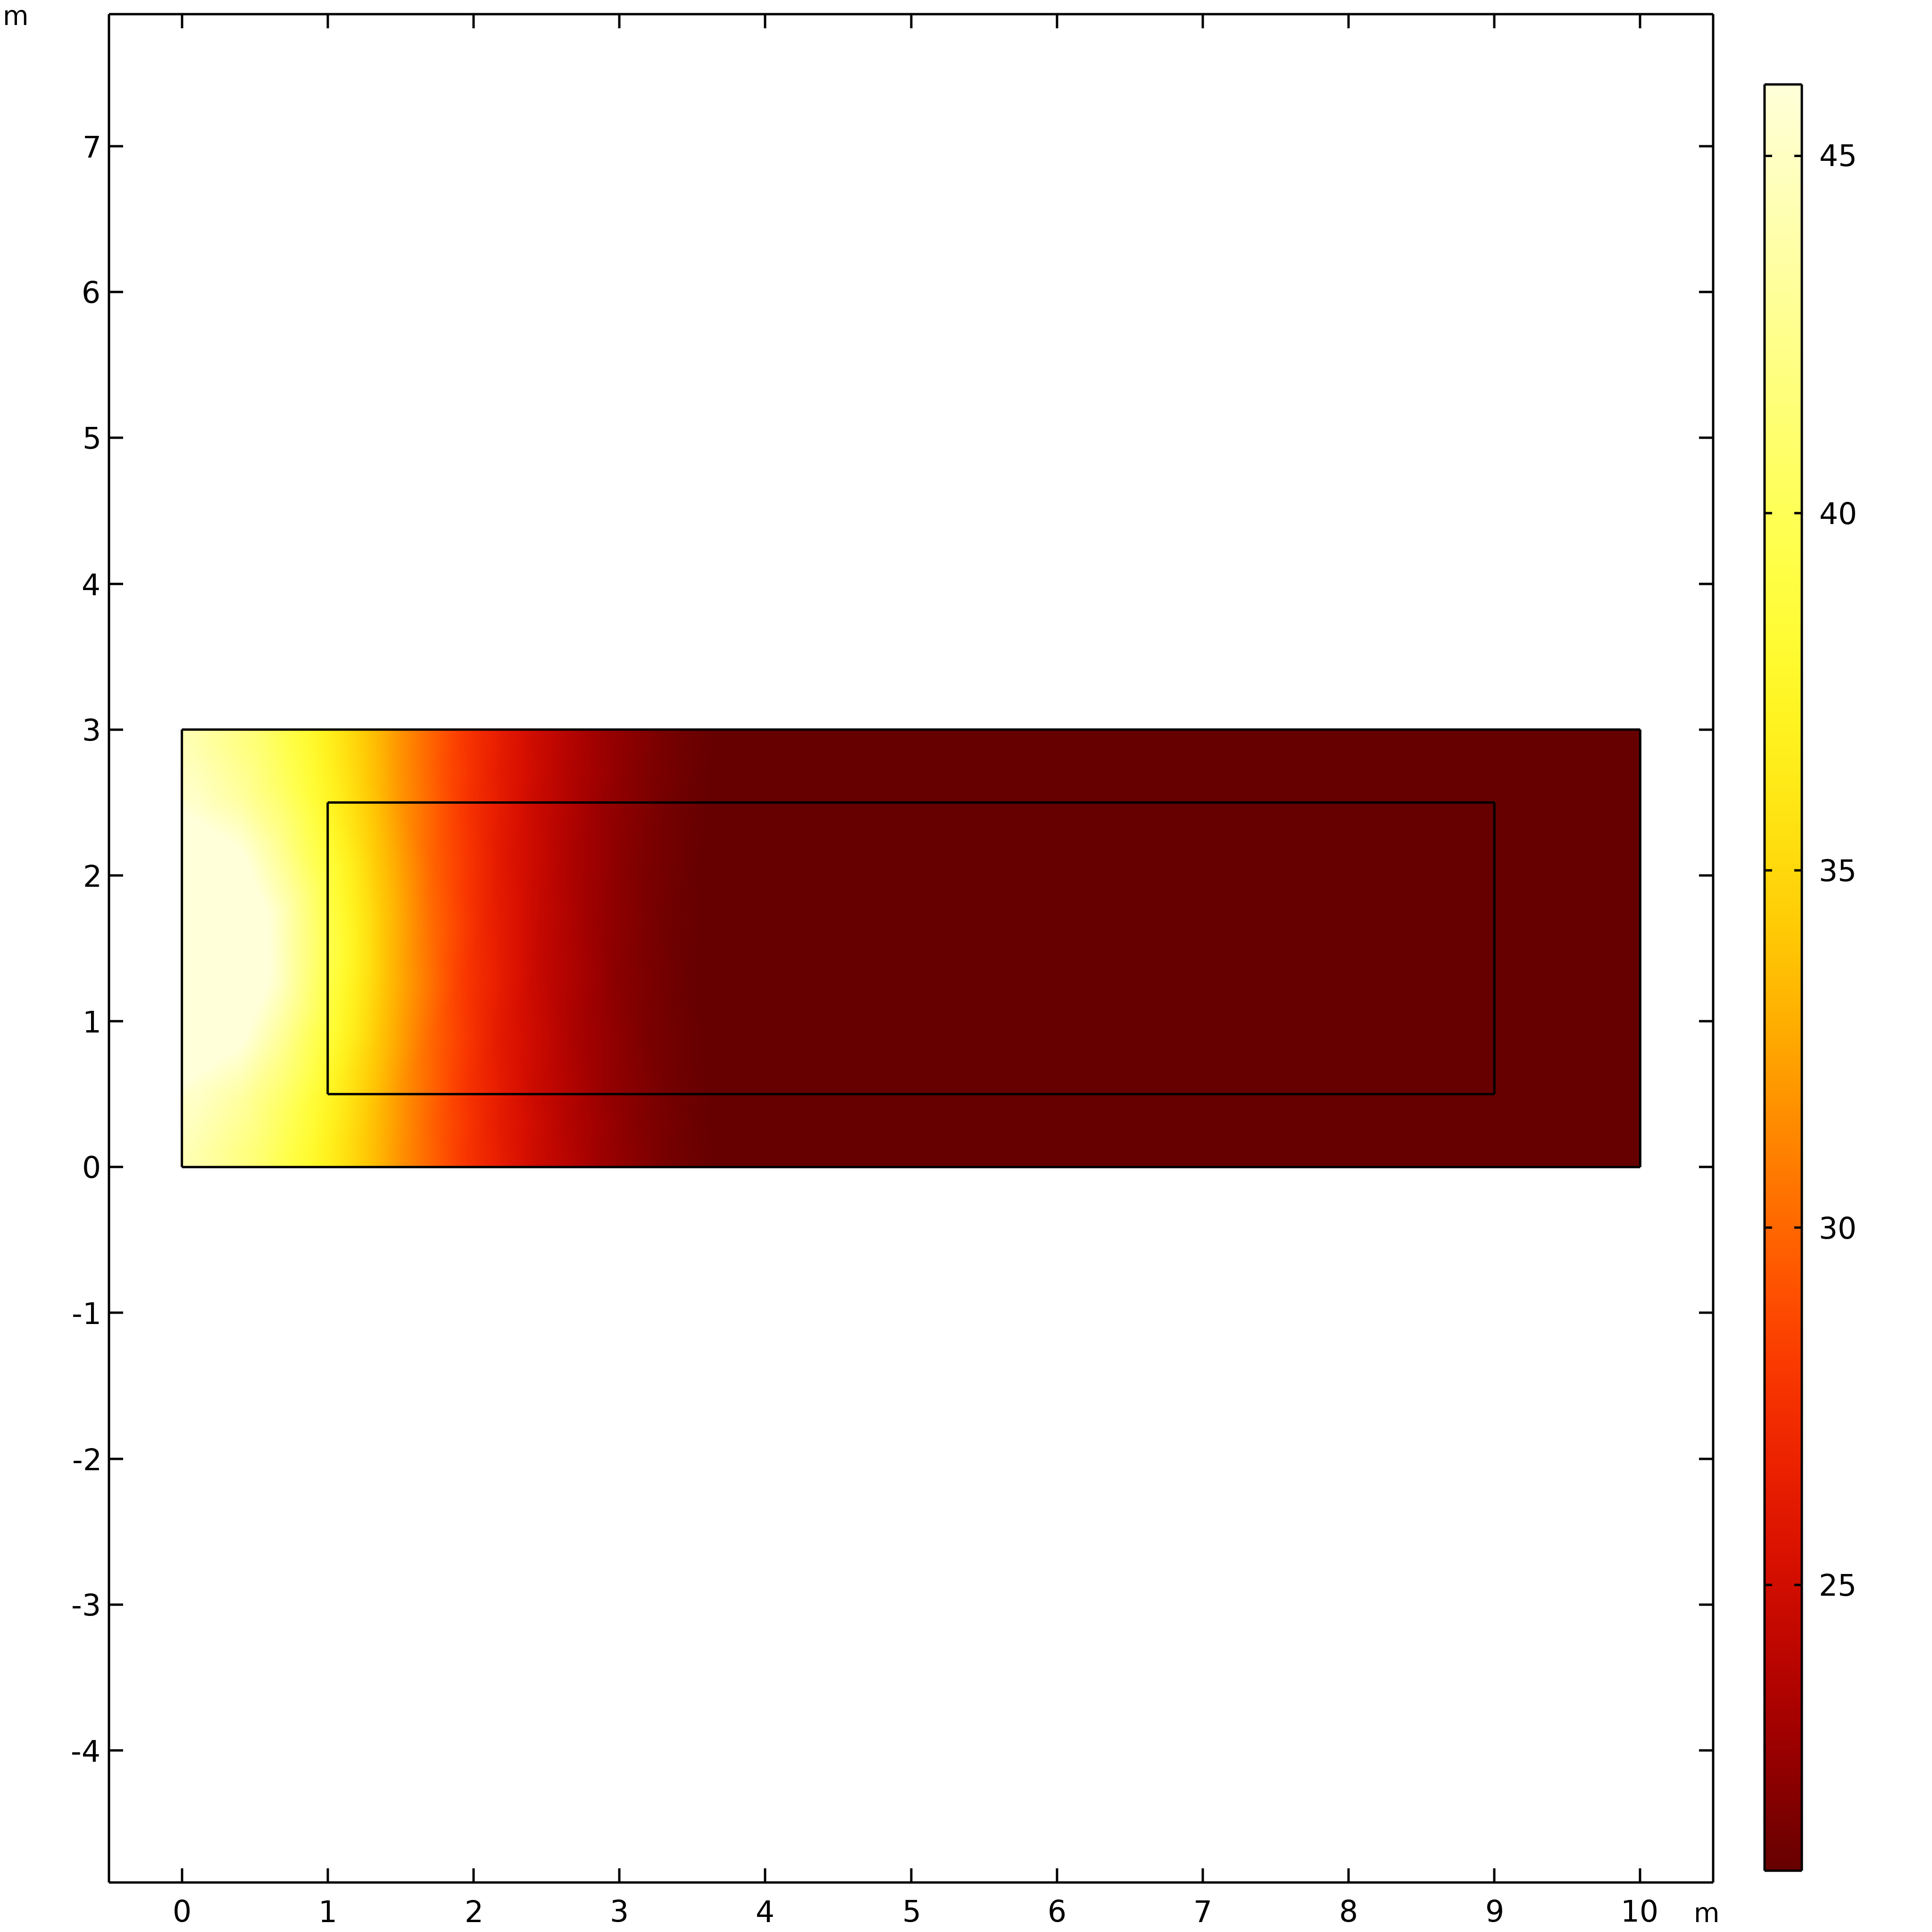
\includegraphics[width=0.4\textwidth]{figures/Temperature Distribution Plot at 01m Cross-Section of the Crop Greenhouse2.png}
         \label{Temperature Distribution Plot at 0.1m Cross-Section of the Glass Greenhouse with Cultivated Crops at a Wind Speed of 3m/s}
      }
       \caption{Temperature Distribution Plot at the Glass Greenhouse with Cultivated Crops at a Wind Speed of 3m/s}
        \label{Temperature Distribution Plot at Cross-Section of the Glass Greenhouse with Cultivated Crops at a Wind Speed of 3m/s.}
  \end{figure}

%风速图
\begin{figure}[htbp]
      \centering
      \subfigure[0.5m Cross-Section of the Glass Greenhouse] { 
          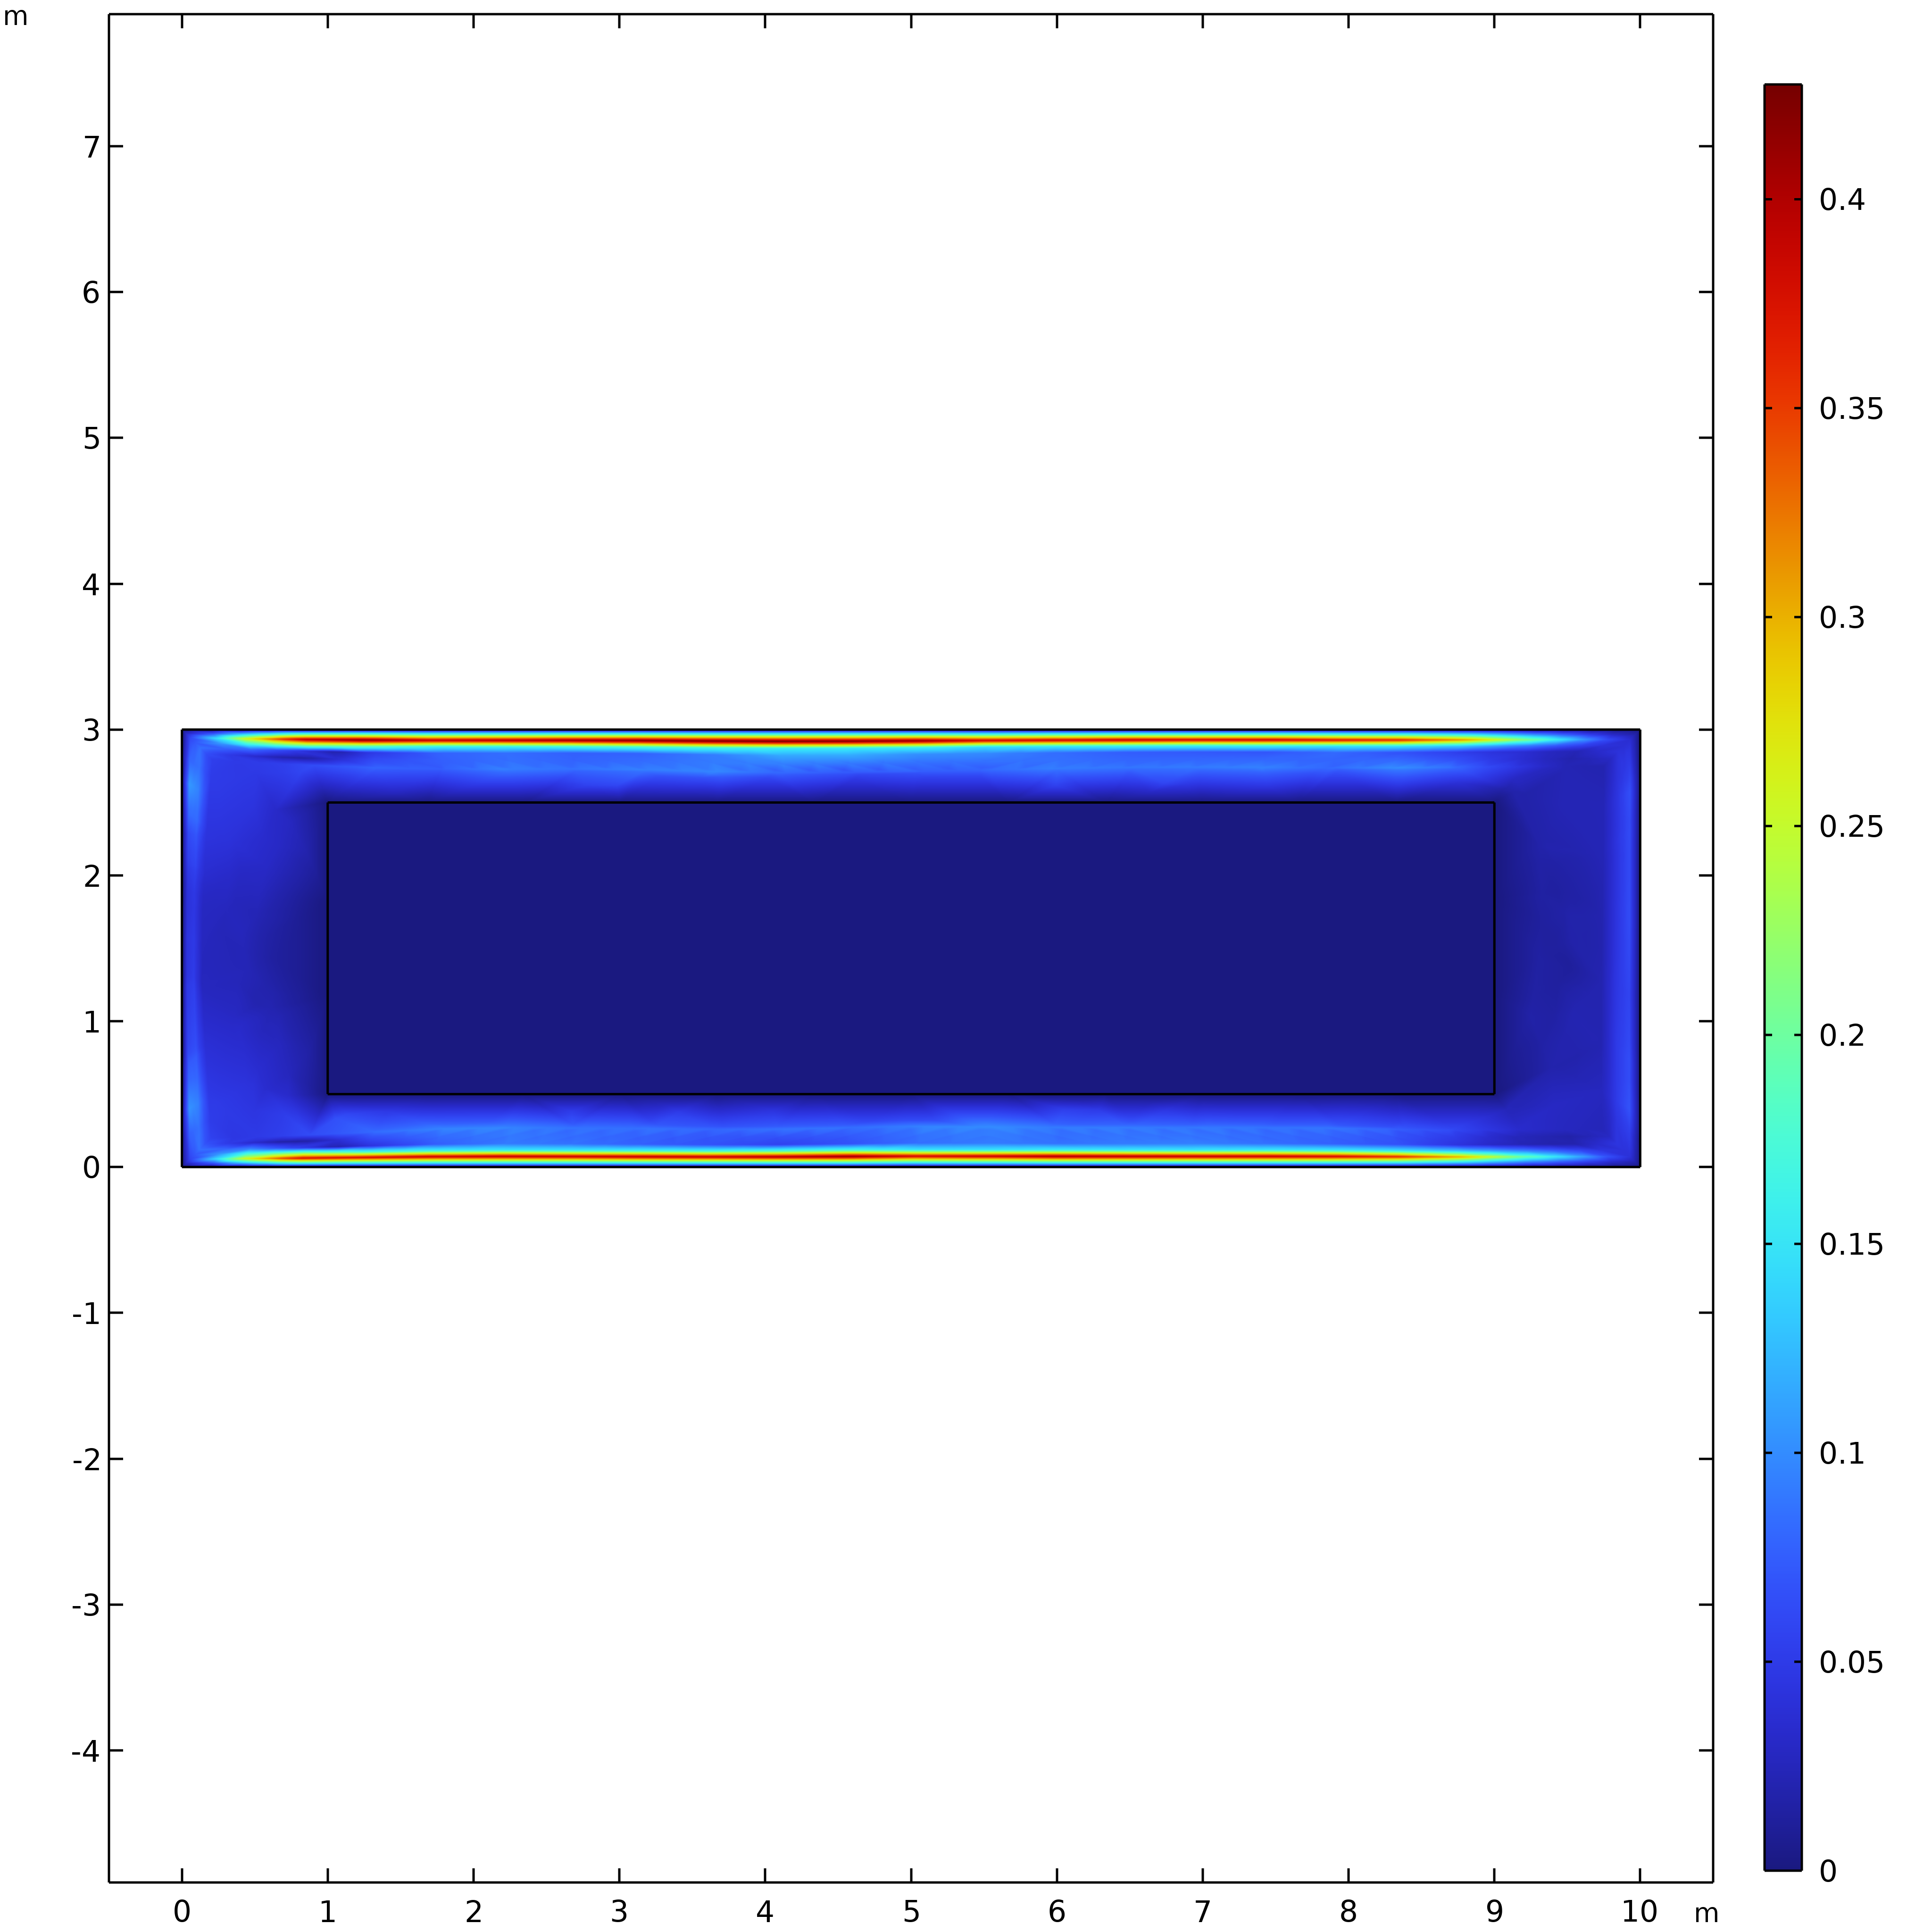
\includegraphics[width=0.4\textwidth]{figures/Wind Speed Distribution Plot at 05m Cross-Section of the Crop Greenhouse2.png}
          \label{Wind Speed Distribution Plot at 0.5m Cross-Section of the Glass Greenhouse with Cultivated Crops at a Wind Speed of 3m/s}
          
      }
       \subfigure[0.1m Cross-Section of the Glass Greenhouse] { 
         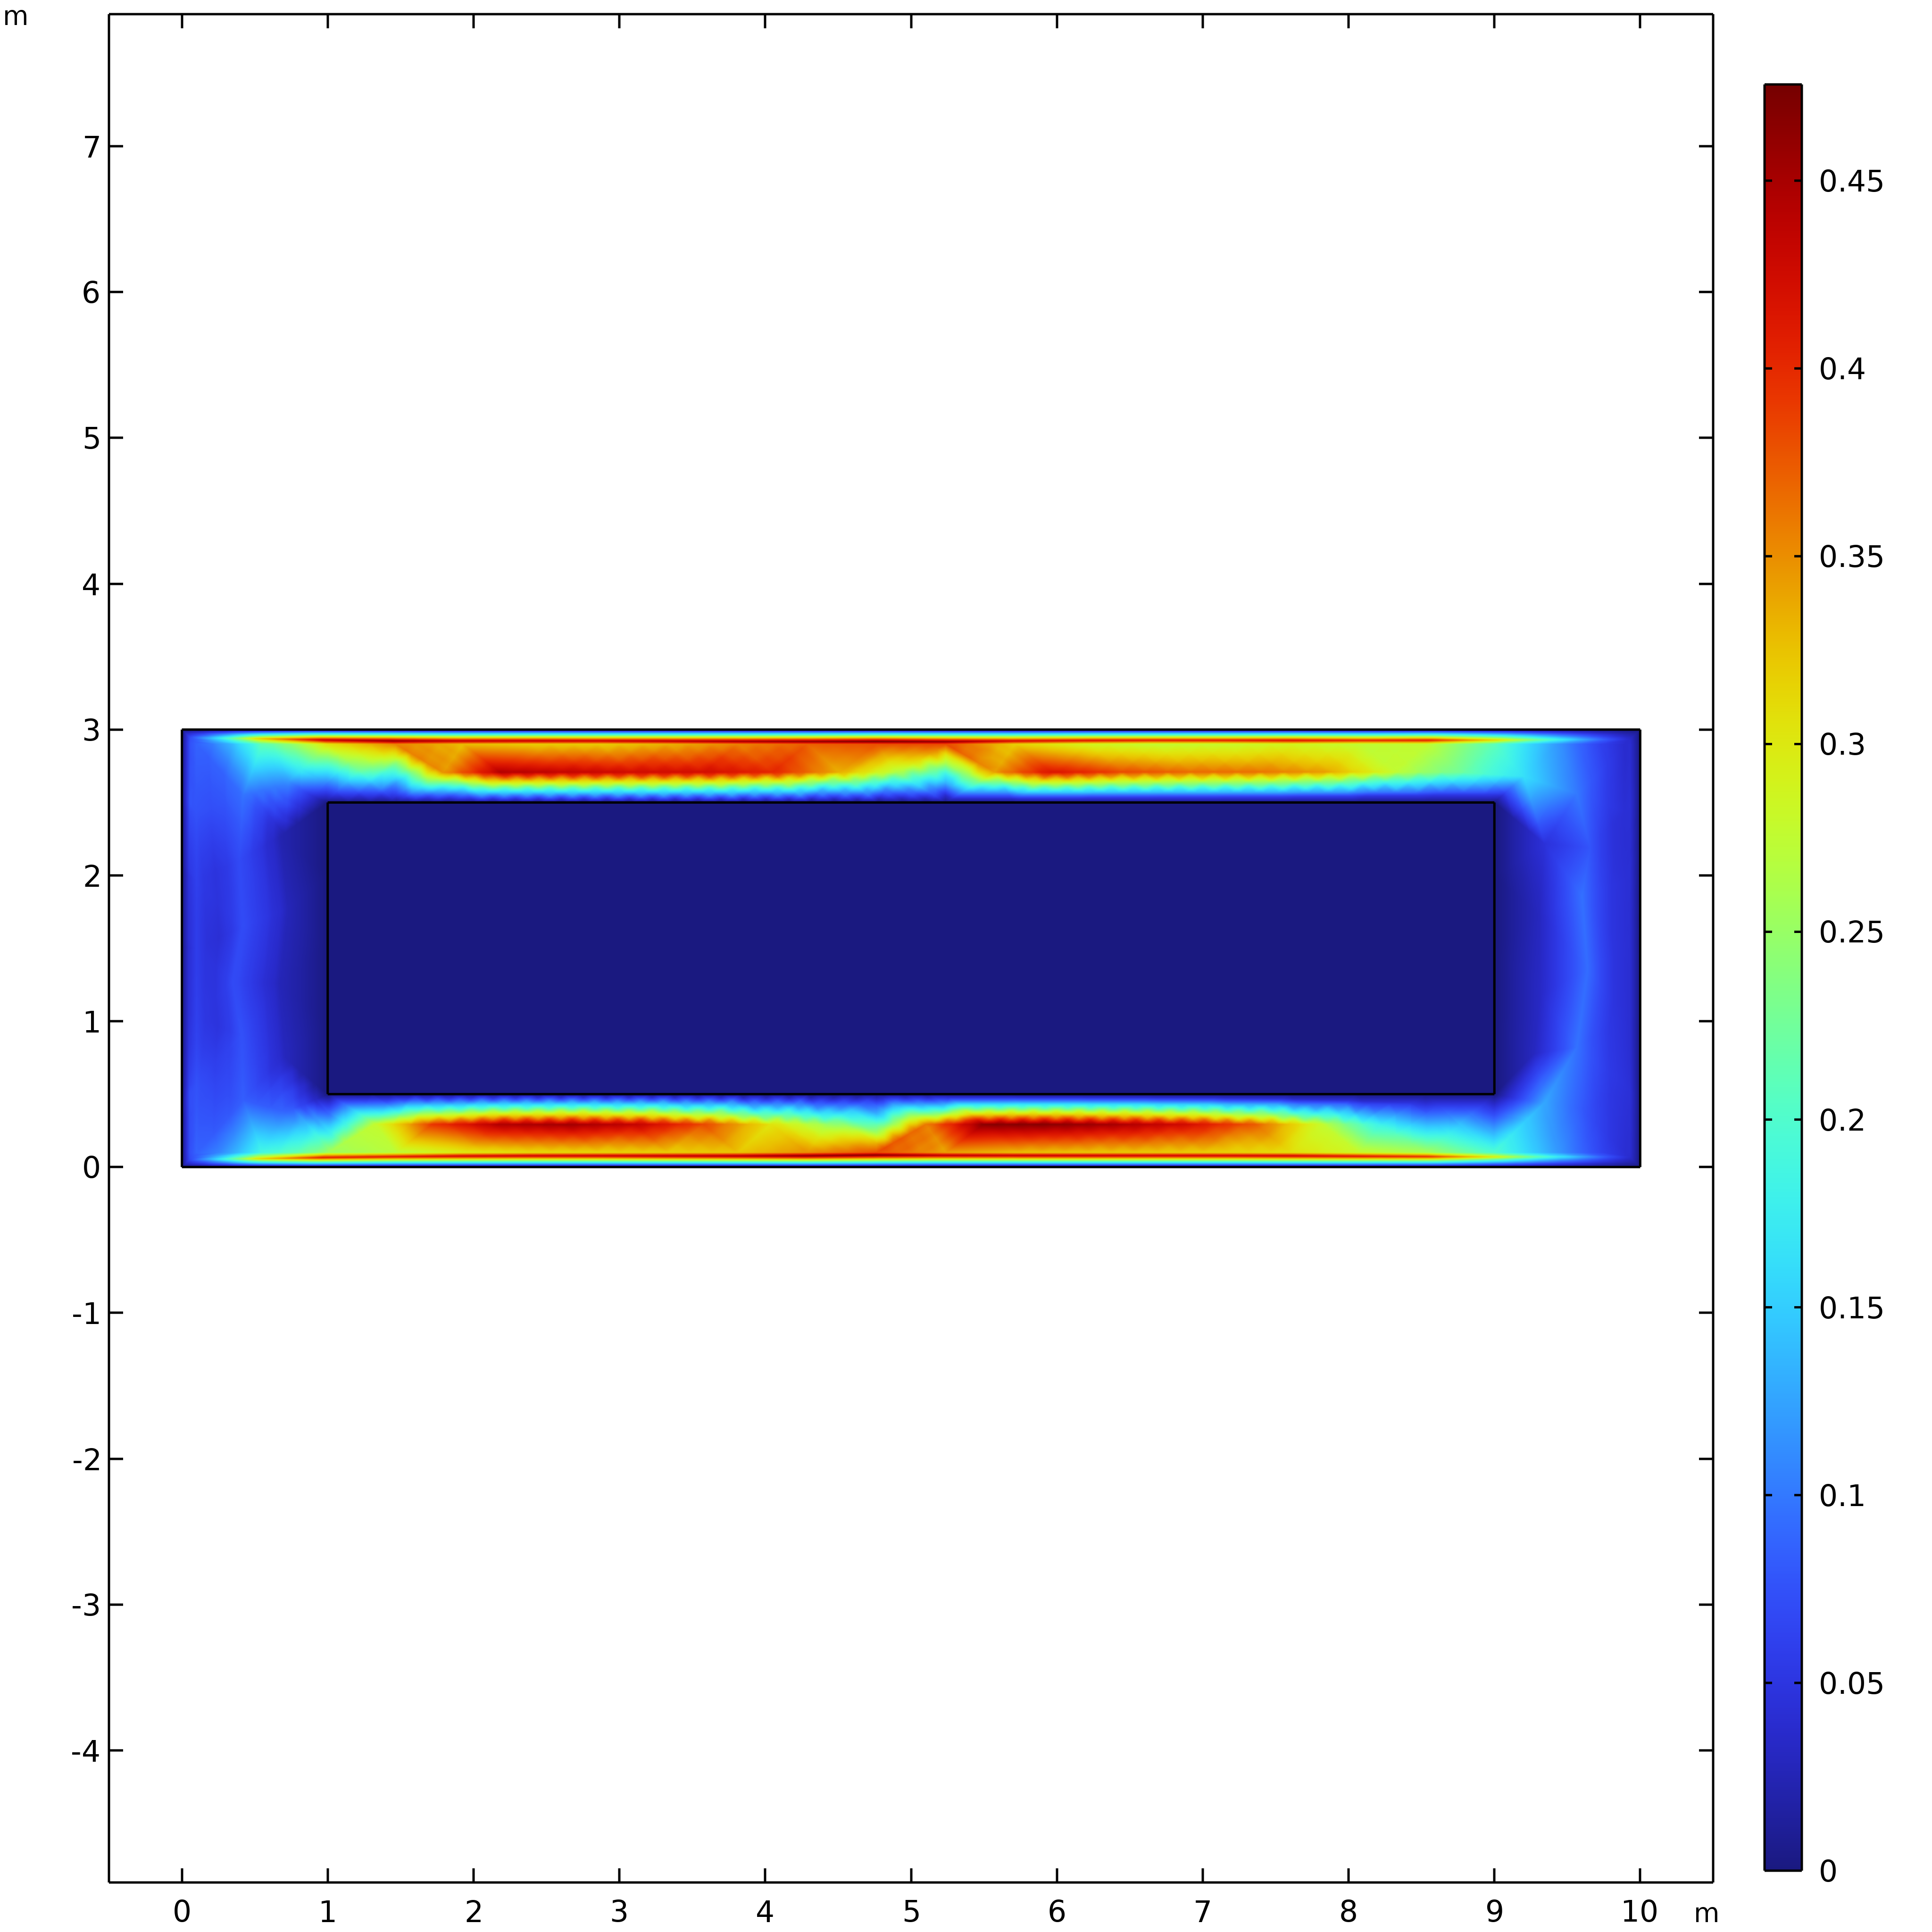
\includegraphics[width=0.4\textwidth]{figures/Wind Speed Distribution Plot at 01m Cross-Section of the Crop Greenhouse2.png}
         \label{Wind Speed Distribution Plot at 0.1m Cross-Section of the Glass Greenhouse with Cultivated Crops at a Wind Speed of 3m/s}
      }
       \caption{Wind Speed Distribution Plot at the Glass Greenhouse with Cultivated Crops at a Wind Speed of 3m/s}
        \label{Wind Speed Distribution Plot at Cross-Section of the Glass Greenhouse with Cultivated Crops at a Wind Speed of 3m/s}
  \end{figure}
  
Combining the temperature distribution plot in Figure \ref{Temperature Distribution Plot at 0.1m Cross-Section of the Glass Greenhouse with Cultivated Crops at a Wind Speed of 3m/s} and the wind speed distribution plot in Figure \ref{Wind Speed Distribution Plot at Cross-Section of the Glass Greenhouse with Cultivated Crops at a Wind Speed of 3m/s}, it is evident that the increase in the outlet wind speed from 2m/s to 3m/s has not led to significant temperature variations. Most areas continue to be suitable for plant growth. At 0.5m above the ground, the average air velocity remains at 0.2m/s, falling below the optimal wind speed of 0.31m/s. However, at 0.1m above the ground, the average airflow velocity reaches 0.32m/s, approaching the optimal wind speed. This results in an adequate wind speed within the crop canopy. In summary, under these conditions, the temperature remains conducive to plant growth, and although the wind speed is faster than the 2m/s outlet speed, it still falls within the relatively slow range. In comparison to the original scenario, this setup continues to provide a favorable environment for plant growth.
% 以下数据全是编的,我只求合理即可!!!!
% 结合下图\ref{Temperature Distribution Plot at 0.1m Cross-Section of the Glass Greenhouse with Cultivated Crops at a Wind Speed of 3m/s}与\ref{Wind Speed Distribution Plot at Cross-Section of the Glass Greenhouse with Cultivated Crops at a Wind Speed of 3m/s},可以看出出风口速度由2m /s增加到3m/s,温度没有很大的变化,大部分地区适合植物生长,在距离地面 0.5 m 处的平均空气流速0.2m/s低于0.31m/s的最佳风速,在距离地面0.1 m 处气流平均流速为0.32m/s接近最佳风速,作物冠层内部风速合适,总而言之该条件下温度合适,风速较为出风口速度2m/s较快,但还偏慢,相较于原来场景,这个场景还是很适合植物生长。




\subsubsection*{The simulation results for ventilation at 1m with a wind speed of 2m/s}
% 通风口位于1m,通风2m/s的仿真结果

% 温度图
\begin{figure}[htbp]
      \centering
      \subfigure[0.5m Cross-Section of the Glass Greenhouse] { 
          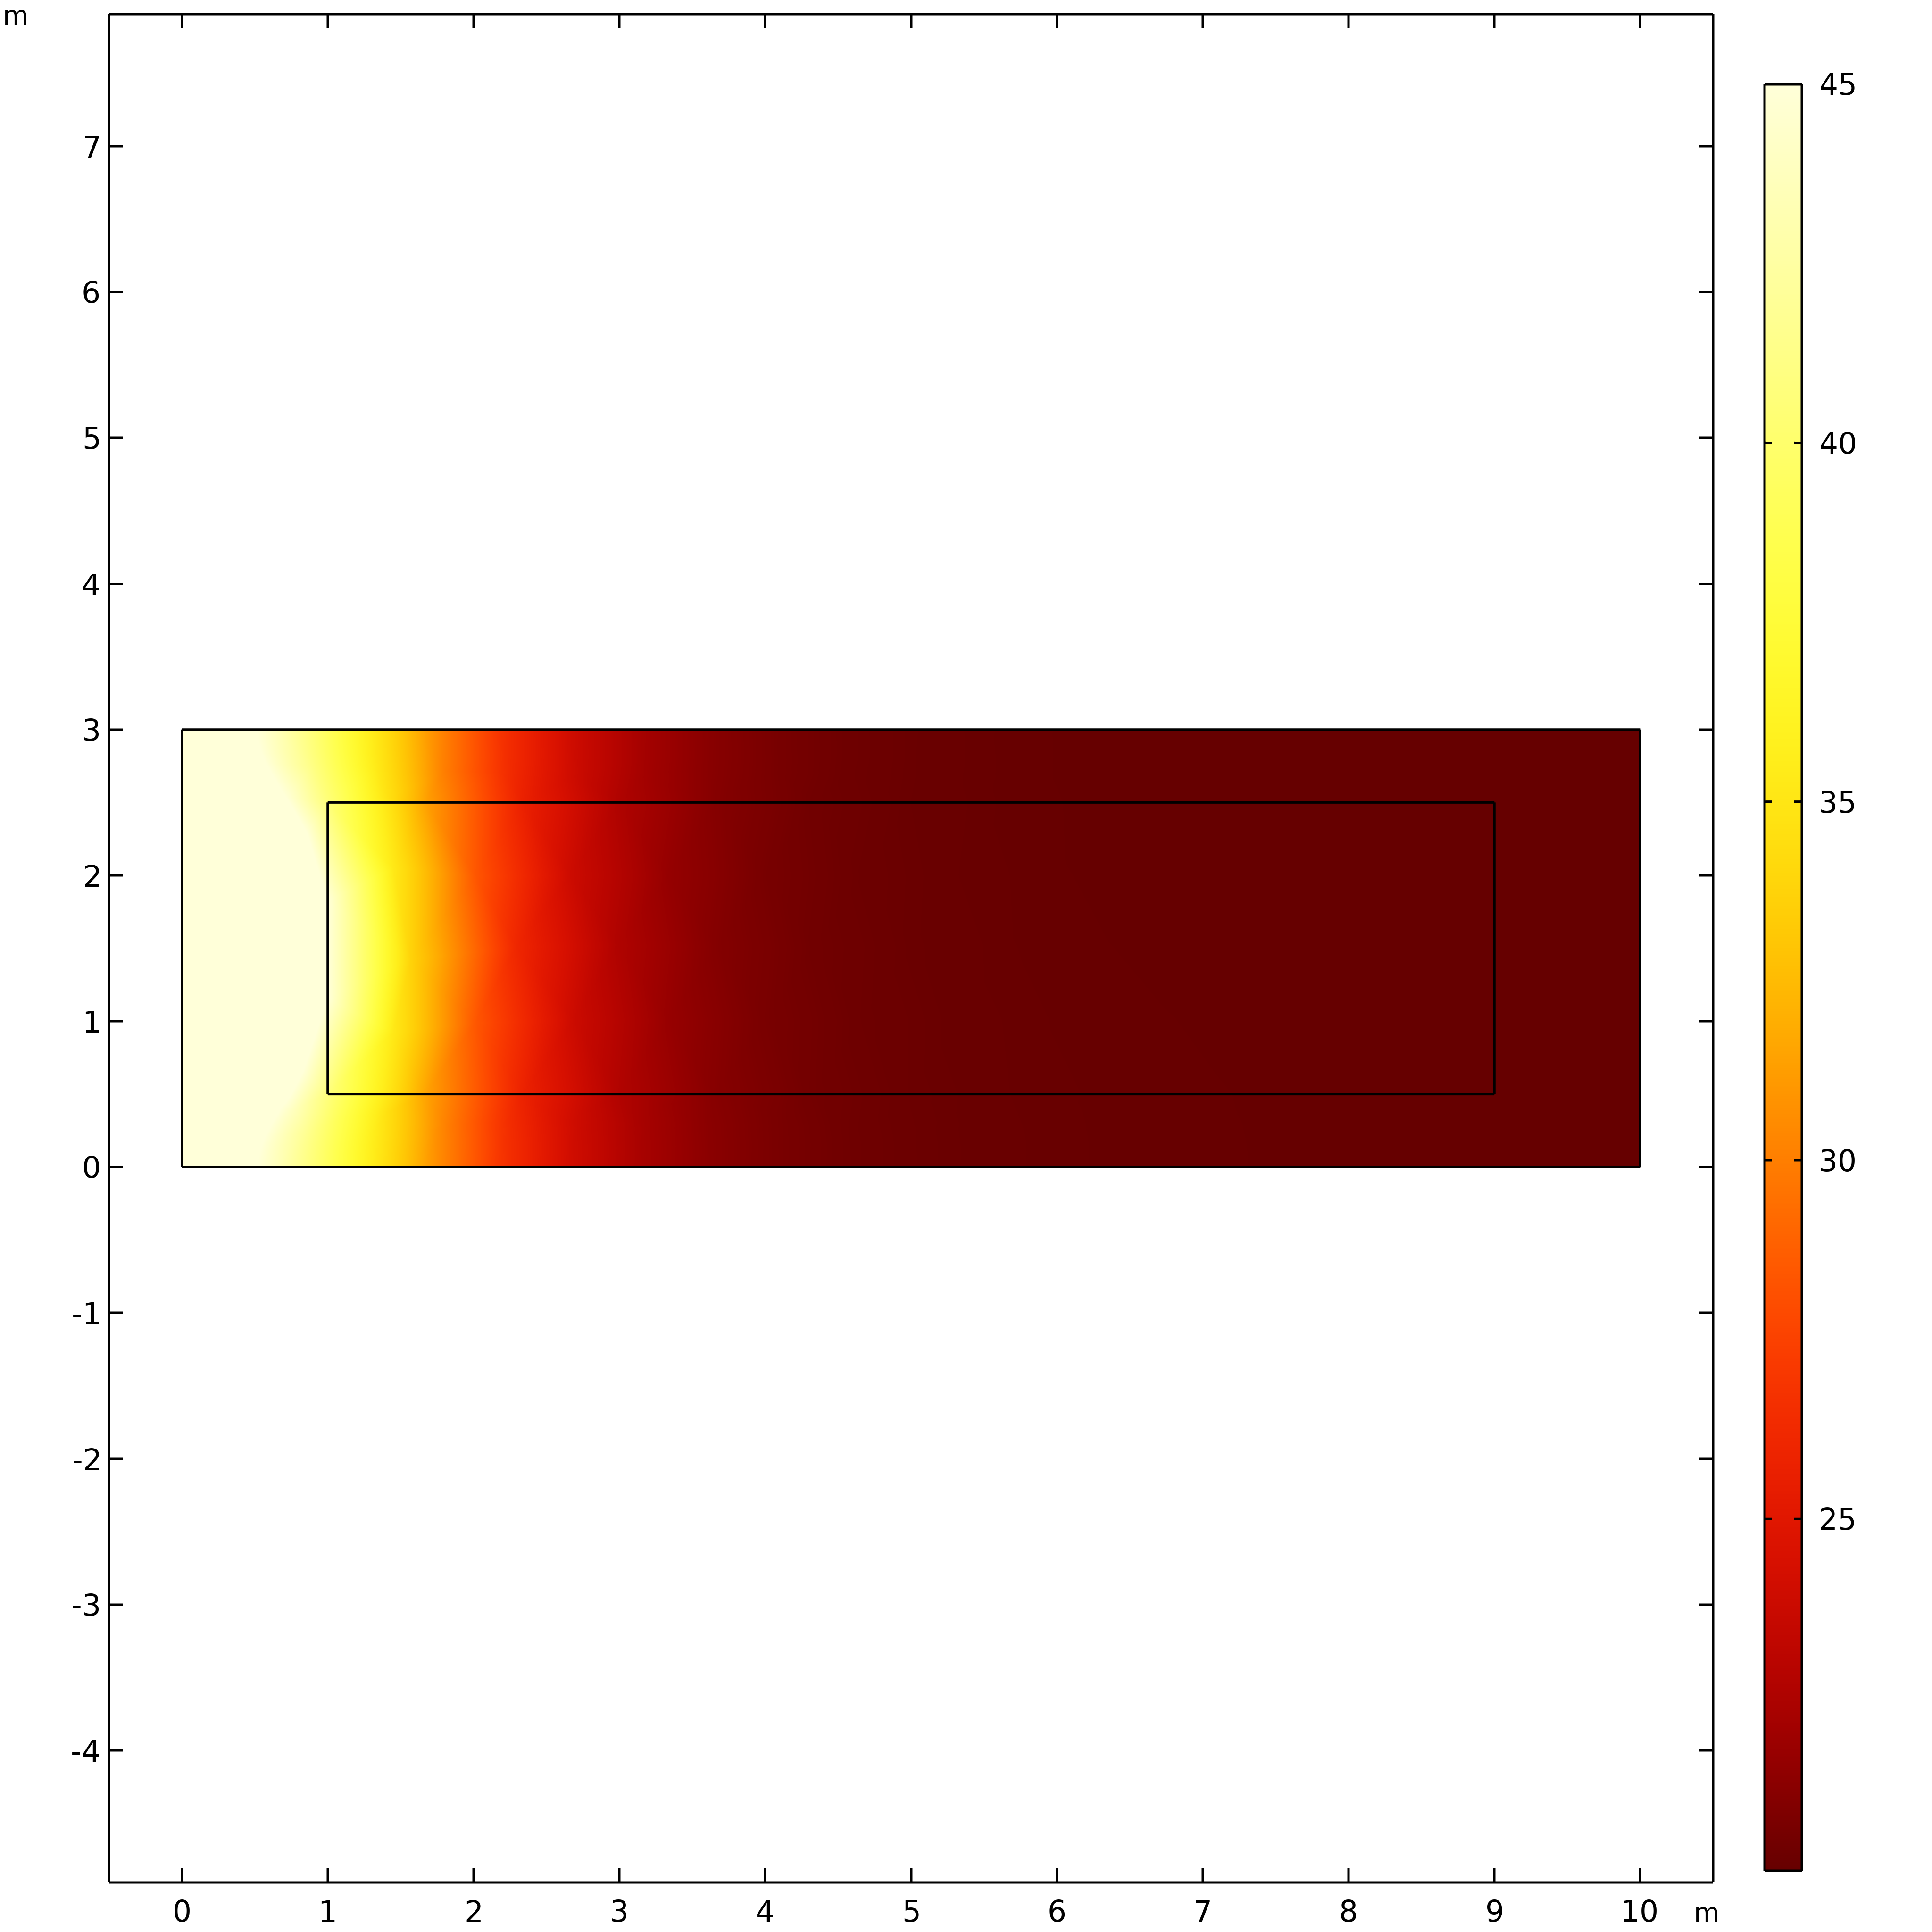
\includegraphics[width=0.4\textwidth]{figures/Temperature Distribution Plot at 05m Cross-Section of the Crop Greenhouse3.png}
          \label{Temperature Distribution Plot at 0.5m Cross-Section of the Glass Greenhouse with Cultivated Crops at a Warm Air Inlet of 1m}
          
      }
       \subfigure[0.1m Cross-Section of the Glass Greenhouse] { 
         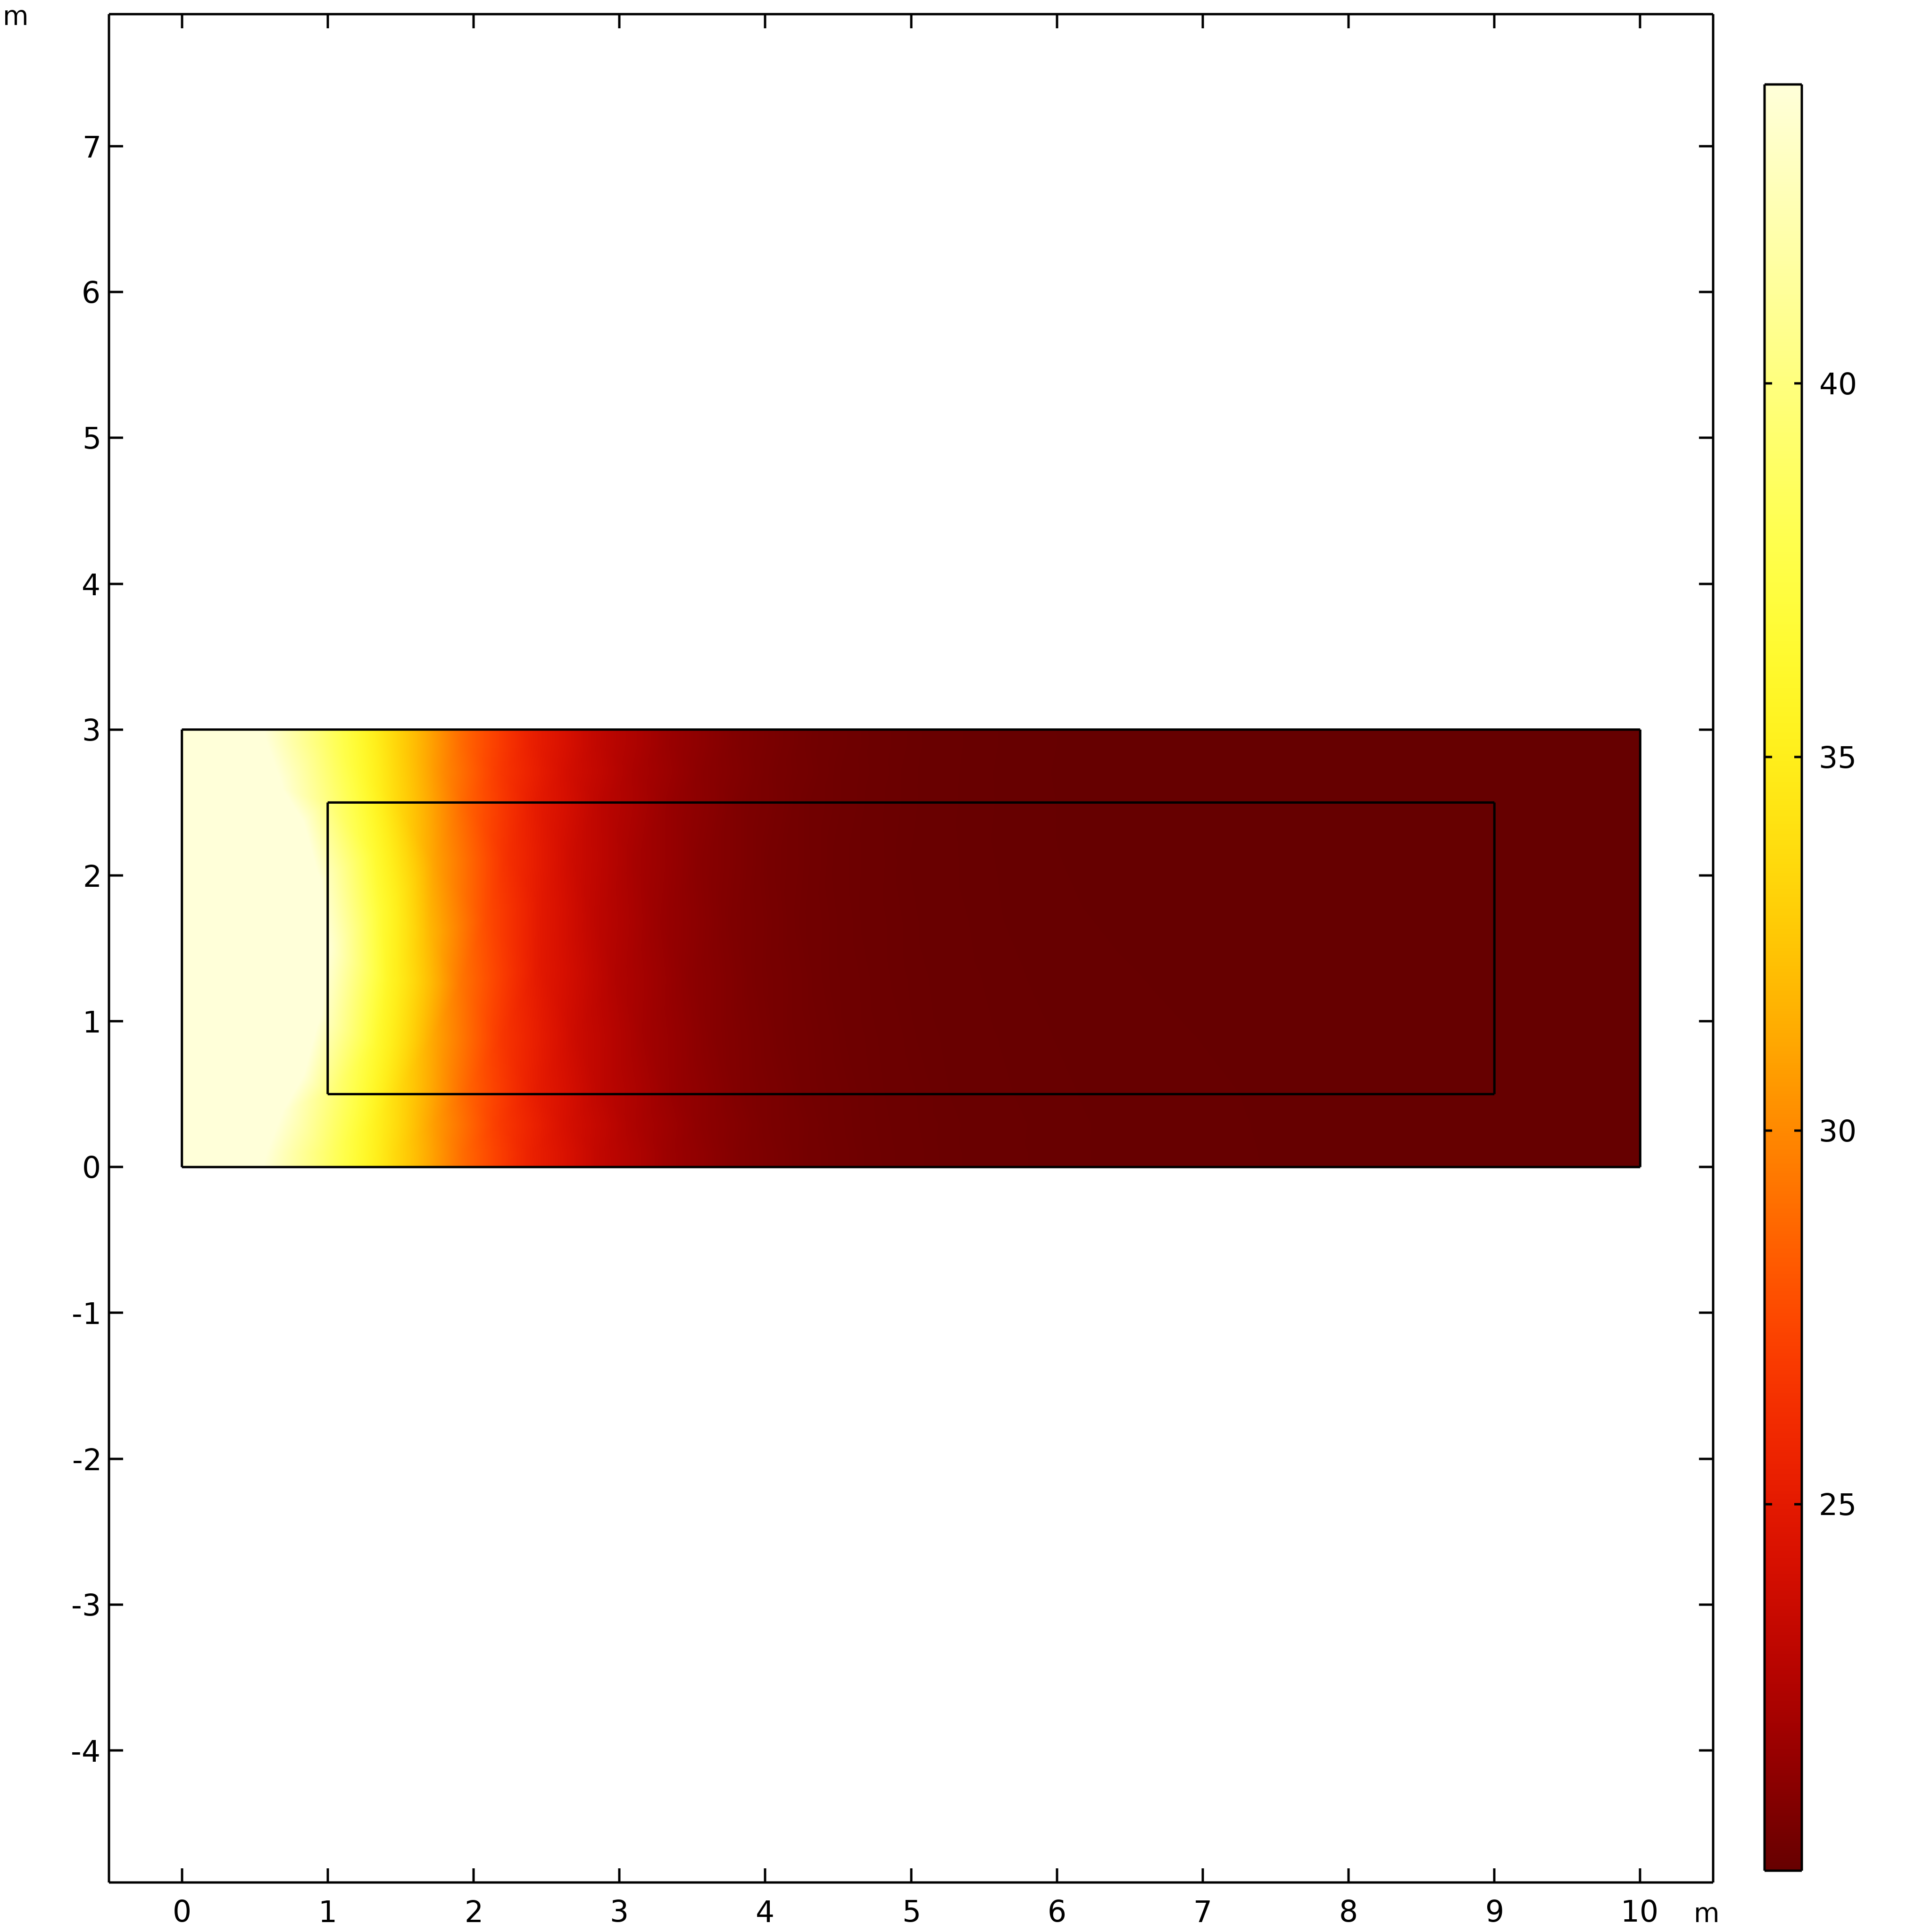
\includegraphics[width=0.4\textwidth]{figures/Temperature Distribution Plot at 01m Cross-Section of the Crop Greenhouse3.png}
         \label{Temperature Distribution Plot at 0.1m Cross-Section of the Glass Greenhouse with Cultivated Crops at a Warm Air Inlet of 1m}
      }
       \caption{Temperature Distribution Plot at the Glass Greenhouse with Cultivated Crops at a Warm Air Inlet of 1m}
        \label{Temperature Distribution Plot at the Glass Greenhouse with Cultivated Crops at a Warm Air Inlet of 1m}
  \end{figure}


%风速图
\begin{figure}[htbp]
      \centering
      \subfigure[0.5m Cross-Section of the Glass Greenhouse] { 
          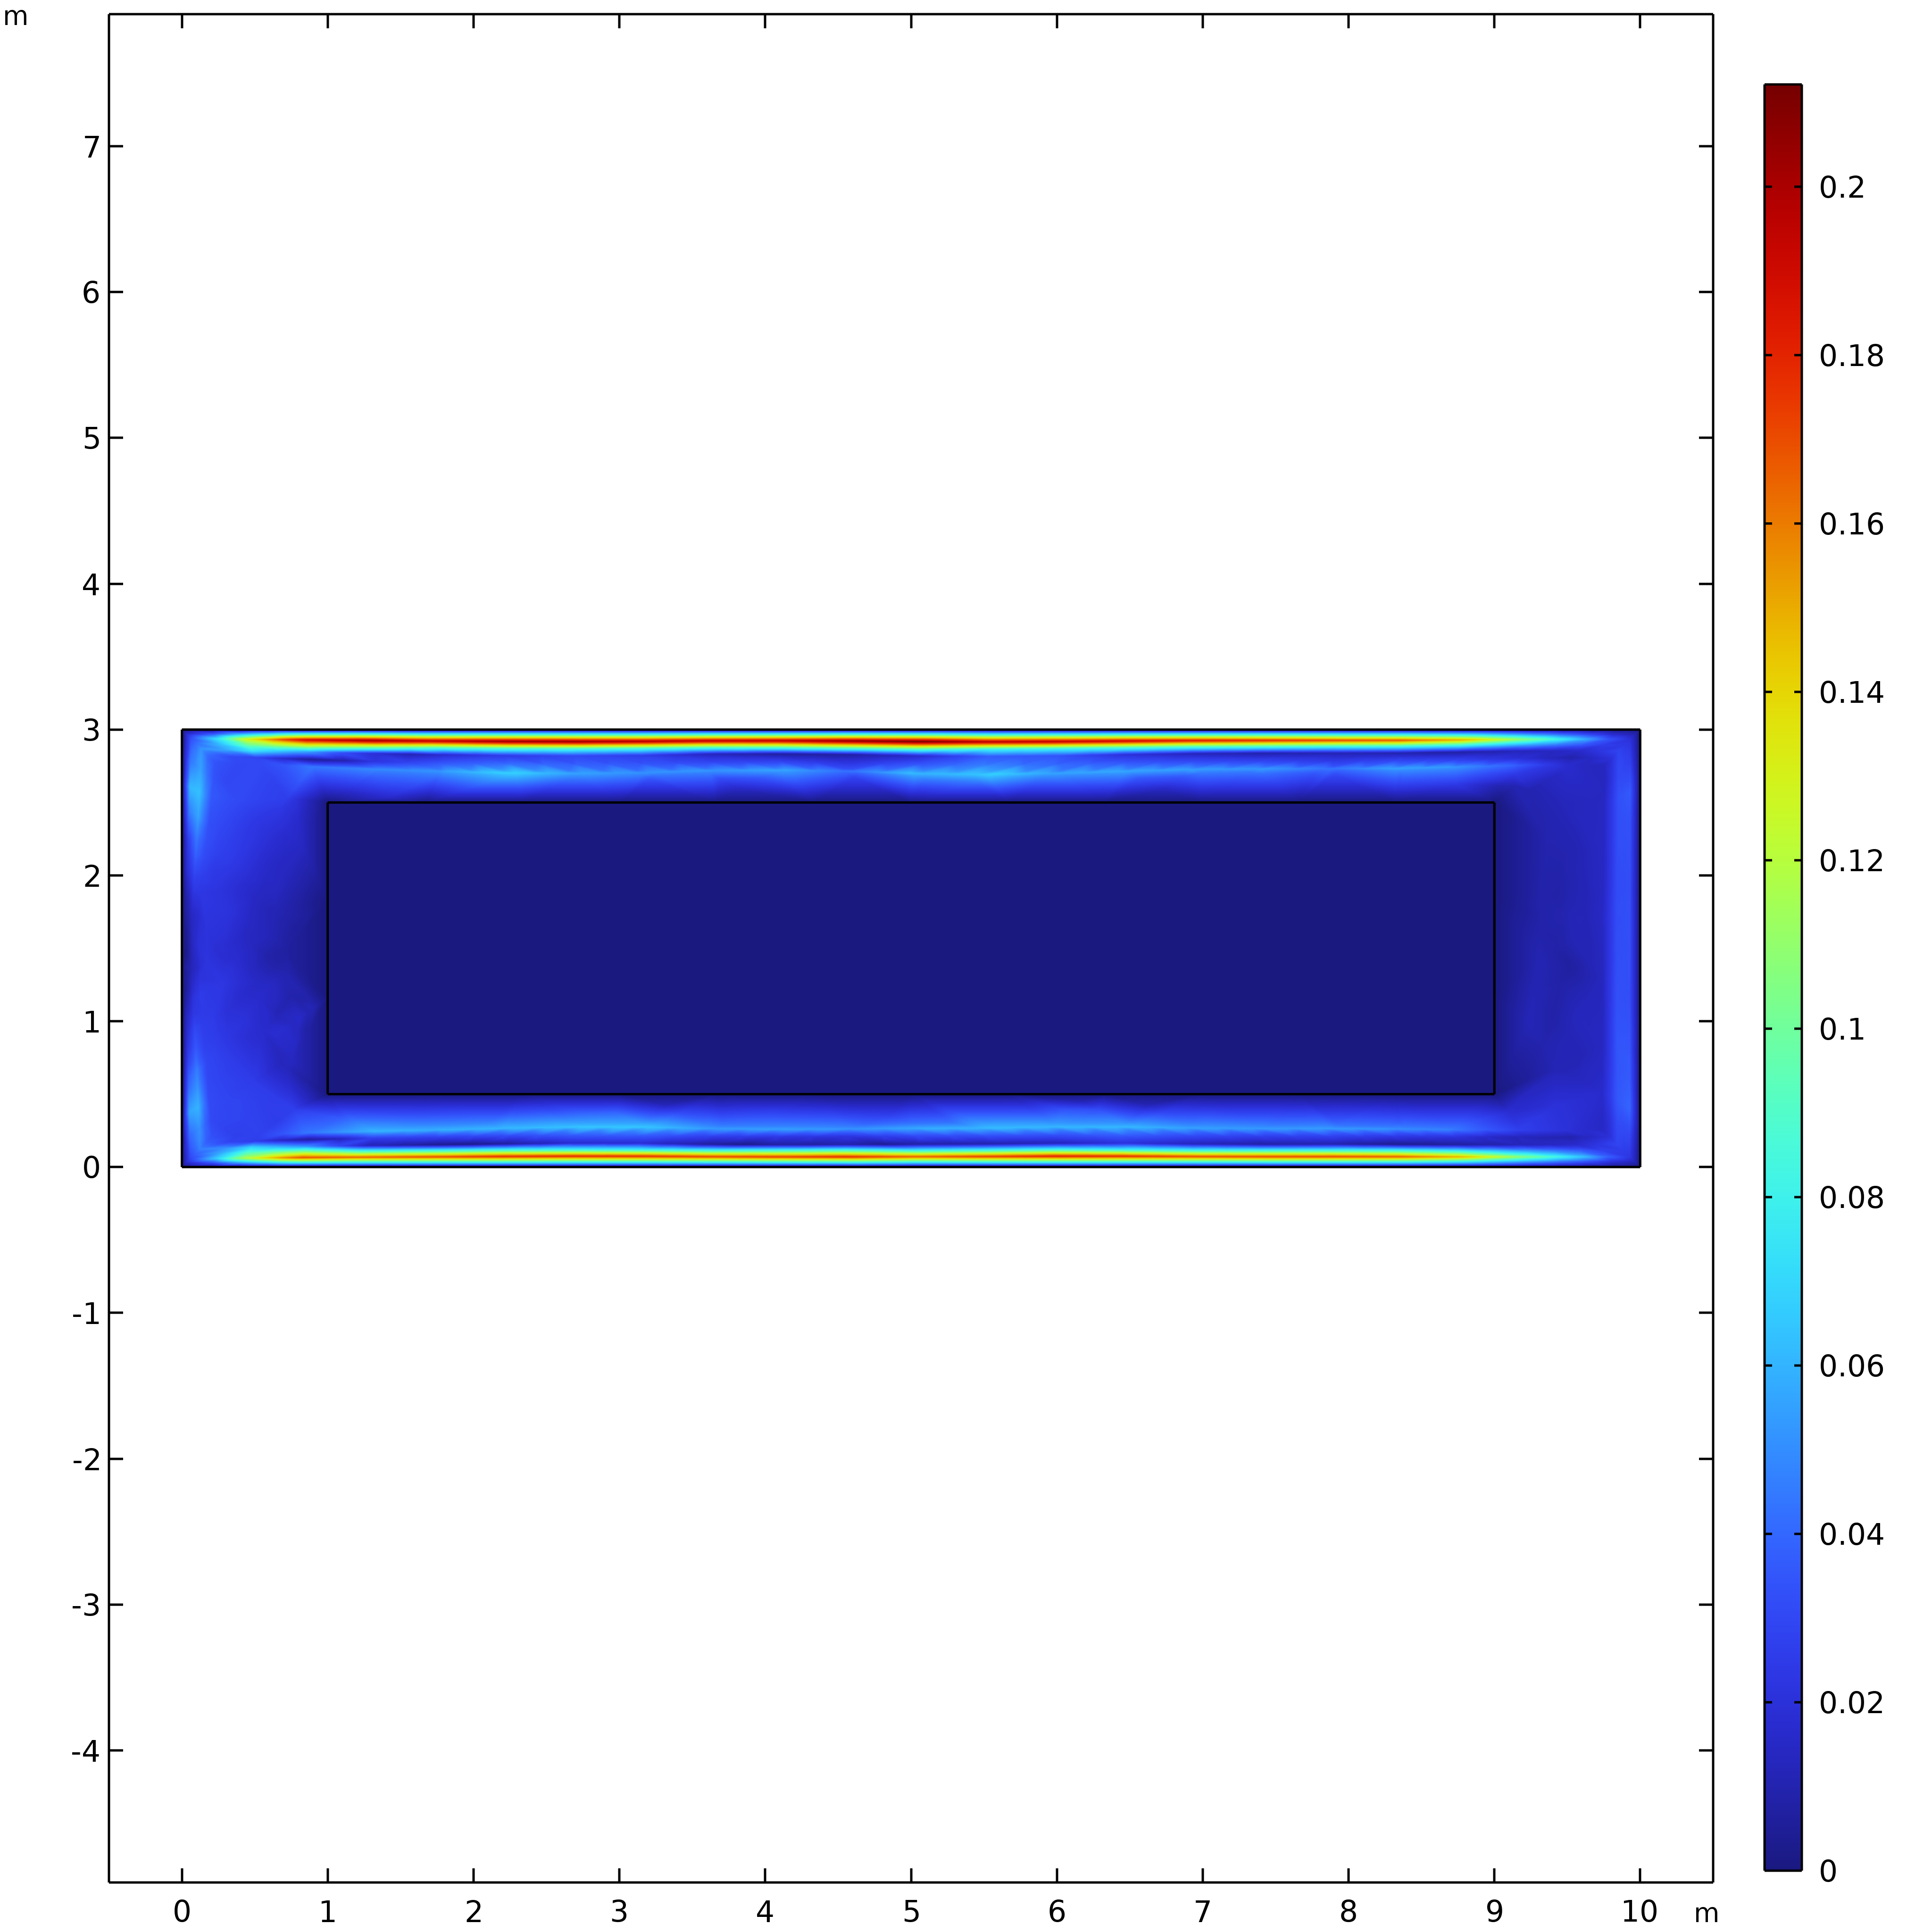
\includegraphics[width=0.4\textwidth]{figures/Wind Speed Distribution Plot at 05m Cross-Section of the Crop Greenhouse3.png}
          \label{Wind Speed Distribution Plot at 0.5m Cross-Section of the Glass Greenhouse with Cultivated Crops at a Warm Air Inlet of 1m}
          
      }
       \subfigure[0.1m Cross-Section of the Glass Greenhouse] { 
         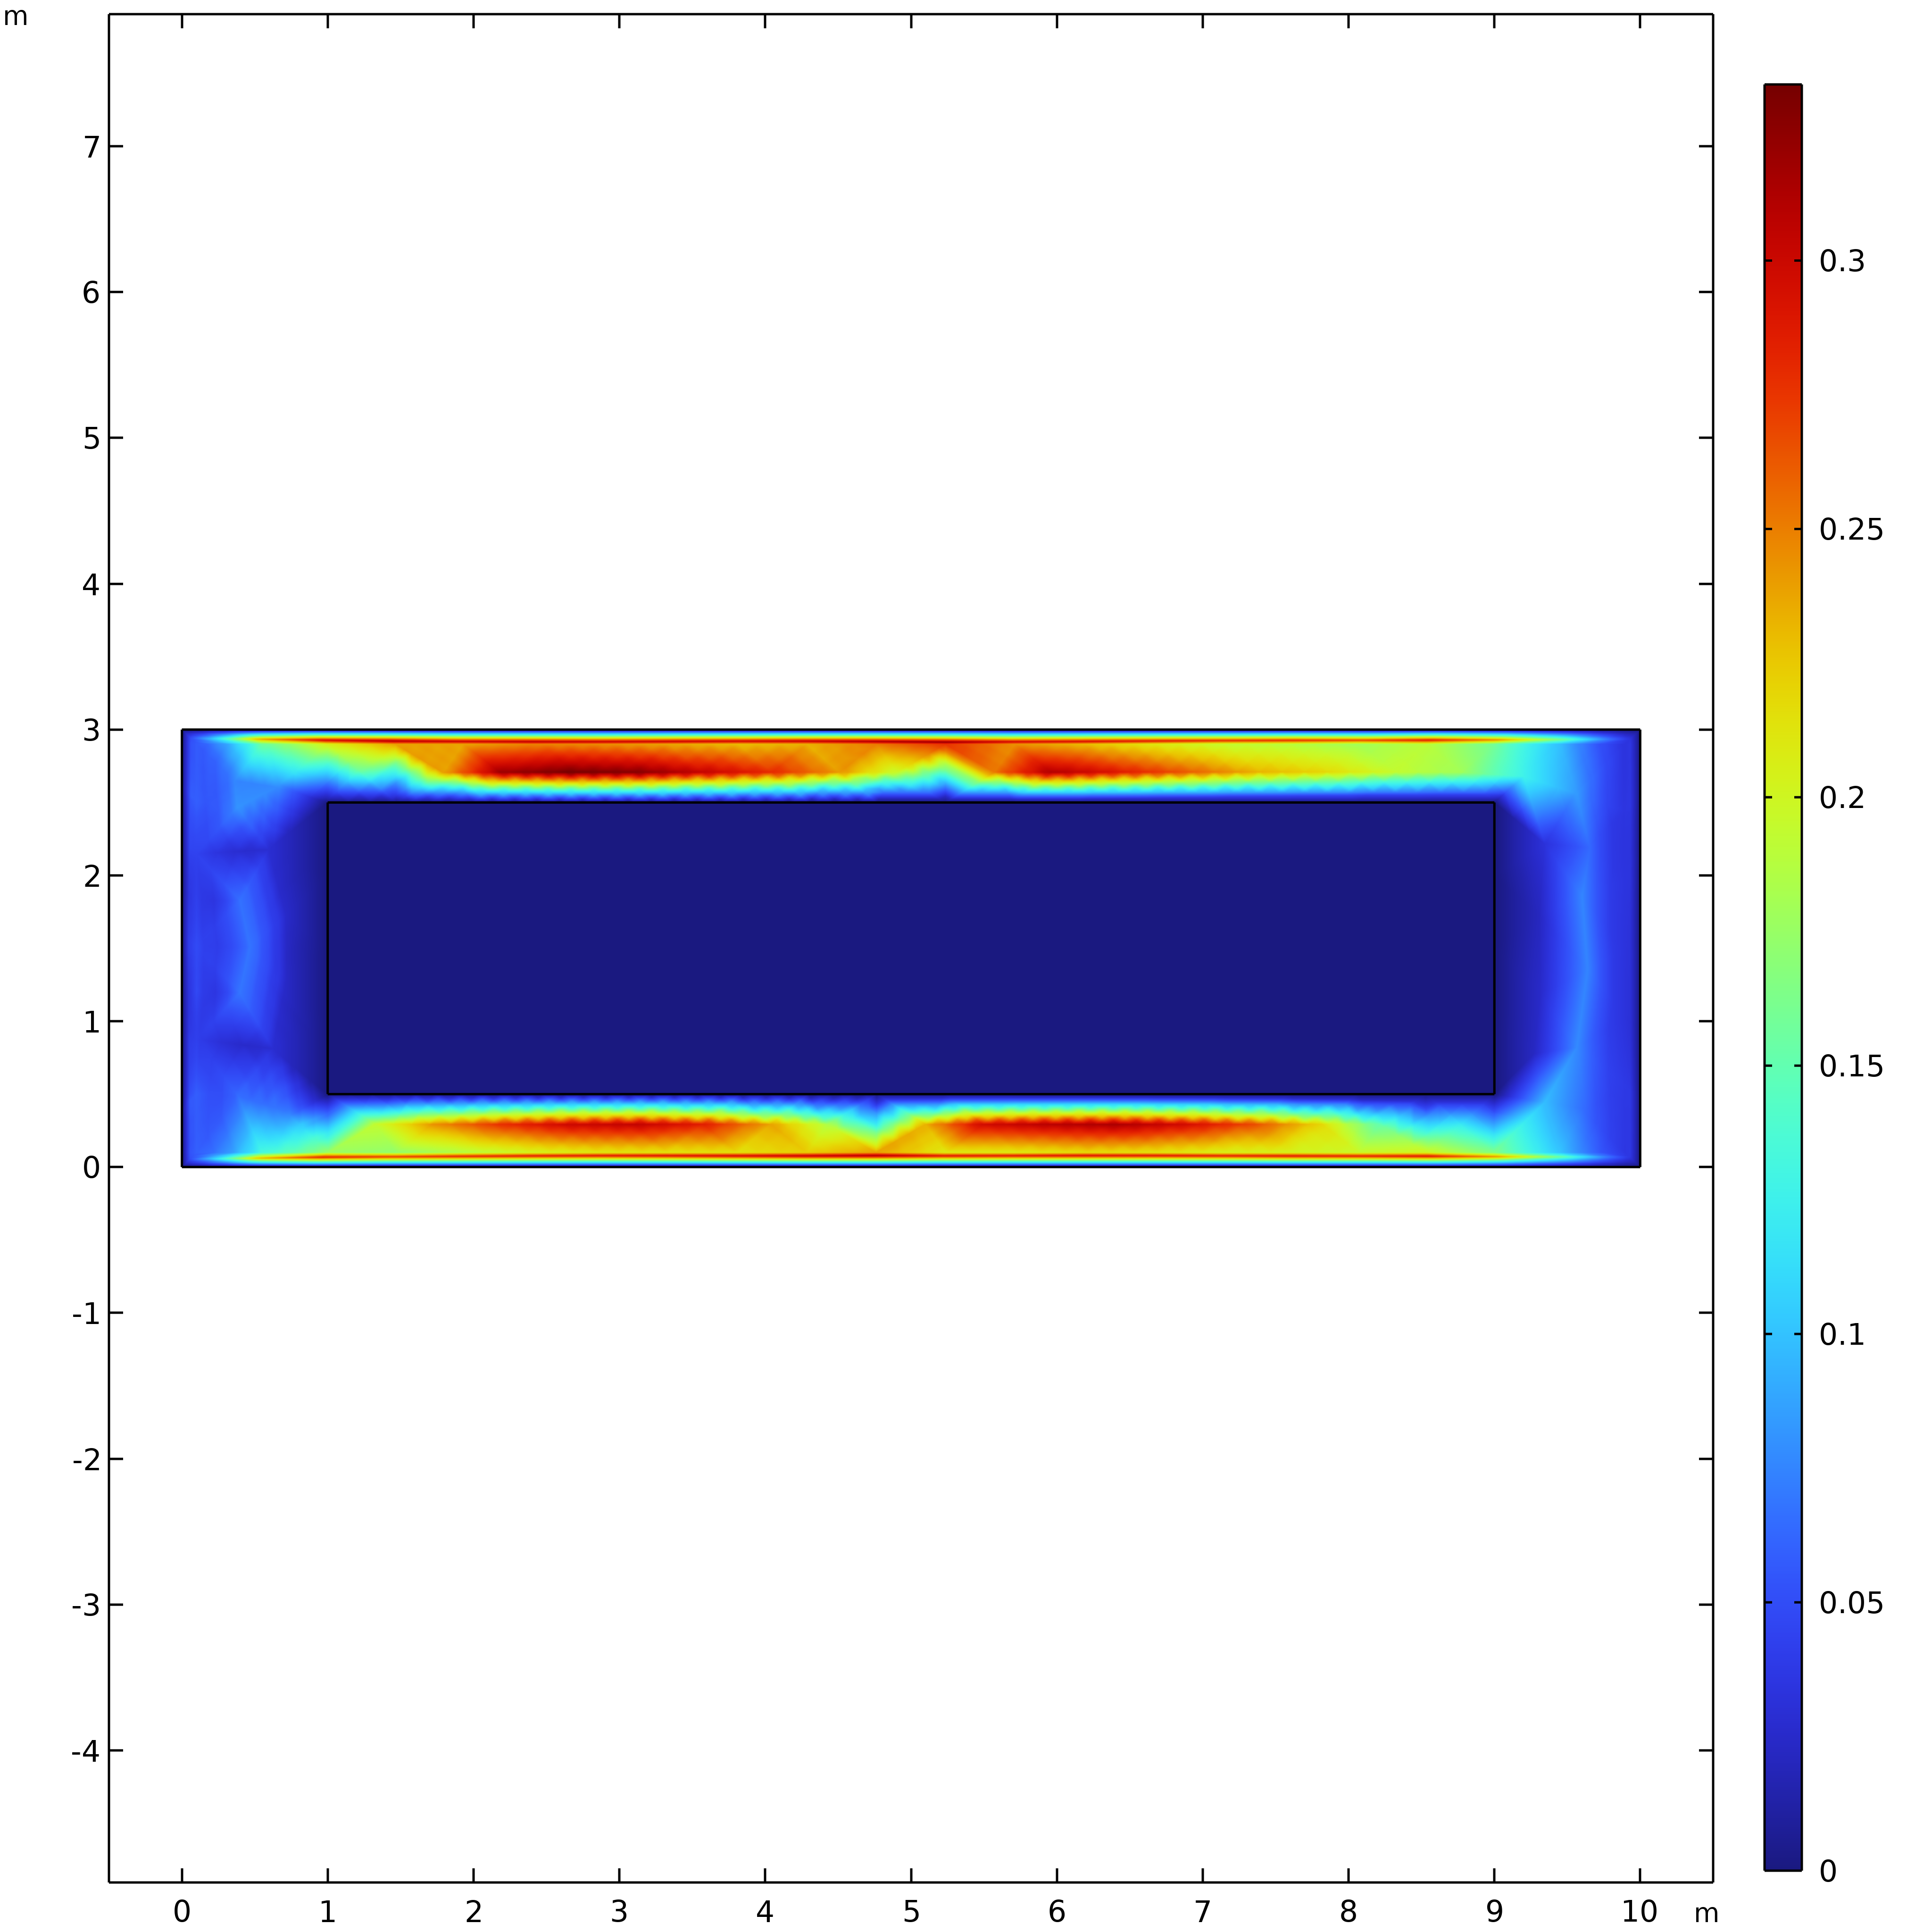
\includegraphics[width=0.4\textwidth]{figures/Wind Speed Distribution Plot at 01m Cross-Section of the Crop Greenhouse3.png}
         \label{Wind Speed Distribution Plot at 0.1m Cross-Section of the Glass Greenhouse with Cultivated Crops at a Warm Air Inlet of 1m}
      }
       \caption{Wind Speed Distribution Plot at the Glass Greenhouse with Cultivated Crops at a Warm Air Inlet of 1m}
        \label{Wind Speed Distribution Plot at Cross-Section of the Glass Greenhouse with Cultivated Crops at a Warm Air Inlet of 1m}
  \end{figure}
  
Combining the temperature distribution plot in Figure \ref{Temperature Distribution Plot at the Glass Greenhouse with Cultivated Crops at a Warm Air Inlet of 1m} and the wind speed distribution plot in Figure \ref{Wind Speed Distribution Plot at Cross-Section of the Glass Greenhouse with Cultivated Crops at a Warm Air Inlet of 1m}, it is evident that with a decrease in the outlet height from 1.3m to 1m, the average temperature increases to 25 degrees. Compared to the other two scenarios, this setup provides a warmer environment. At 0.5m above the ground, the average air velocity approaches the optimal wind speed, exceeding the wind speeds in the original scenario and Scenario 1. This results in suitable wind speeds within the crop canopy. At 0.1m above the ground, the average airflow velocity is 0.33m/s, close to the optimal wind speed, ensuring appropriate wind speeds within the crop canopy. In conclusion, under these conditions, both the temperature and wind speed are suitable. Compared to Scenario 1 and the original scenario, this setup is more favorable for plant growth.
% 以下数据全是编的,我只求合理即可!!!!
% 结合下图\ref{Temperature Distribution Plot at the Glass Greenhouse with Cultivated Crops at a Warm Air Inlet of 1m}与\refWind Speed Distribution Plot at Cross-Section of the Glass Greenhouse with Cultivated Crops at a Warm Air Inlet of 1m},可以看出出风口高度从1.3m下降到1m,平均温度为25度,相较于另外两个场景,这个更加温暖,在距离地面 0.5 m 处的平均空气流速接近最佳风速,比原来场景与场景1的风速都要大,作物冠层风速合适,在距离地面0.1 m 处气流平均流速为0.33m/s接近最佳风速,作物冠层内部风速合适,总而言之该条件下温度合适,风速合适,相较于场景1与原来场景,这个场景更加适合植物生长。



\subsection{Optimize the greenhouse fan design}
% 温室风扇设计优化

\subsubsection{Factors to consider}
% 可以考虑的因素

Optimizing greenhouse fan design can achieve a more stable and controllable greenhouse environment, enhancing the efficiency and quality of plant growth. This is of significant importance for the sustainable development of modern agriculture and improving production yields. The optimization of greenhouse fans can be considered from the following five factors:
% 优化温室风扇设计可以实现更稳定、可控的温室环境,提高植物生长的效率和质量。这对于现代农业的可持续发展和提高生产效益都具有重要意义,优化温室风扇可以从以下5个因素考虑。

\begin{description}
	\item[Fan Placement:] Strategically positioning fans ensures uniform airflow within the greenhouse. This helps eliminate dead corners and zones, ensuring proper ventilation throughout the entire greenhouse. Thoughtful placement of fans allows for better temperature regulation, preventing localized overheating or cooling.
 % 风扇位置 合理安置风扇位置可以确保空气在温室内均匀流动。这有助于避免死角和死区,确保整个温室都能受到适当的通风。通过巧妙地安排风扇,可以更好地调节温室内的温度,防止局部过热或过冷。
    \item[Wind Speed:]Appropriate wind speed plays a crucial role in regulating the temperature within the greenhouse. By controlling the wind speed, overheating can be prevented, especially during periods of high summer temperatures, while still providing the comfortable temperature required for plant growth.% 风速 适当的风速可以帮助调节温室内的温度。通过控制风速,可以防止过热,特别是在夏季高温时,同时提供植物所需的舒适温度。
    
    \item[Number of Fans:]Increasing the number of fans enhances ventilation within the greenhouse, ensuring a more even circulation of air. This is crucial for maintaining optimal climatic conditions. Having more fans allows for a more effective control of the greenhouse temperature.% 风扇数量 增加风扇的数量可以提高温室内的通风效果,确保空气能够更加均匀地流通。这对于维持适宜的气候条件非常重要。更多的风扇可以更有效地调控温室内的温度。
    \item[Air Blowing Temperature:] Precise control of the air-blowing temperature improves energy efficiency, avoids unnecessary energy waste, and provides the most suitable growth conditions for plants. This, in turn, enhances crop yield and quality.
% 吹风温度 通过精确控制吹风温度,可以提高能源利用效率,避免不必要的能源浪费,还可以为植物提供最适宜的生长条件,从而提高作物的产量和质量。
    \item[Crop Cultivation:] Tailoring the design of the fan system to the specific needs of different crops can provide the most favorable growth environment, promoting the growth and development of crops. % 种植作物 针对不同作物的需求,合理设计的风扇系统可以提供最适宜的生长环境,促进作物的生长和发育。
\end{description}

\subsubsection{Optimization Plan}
% 优化方案

Next we discuss some of the factors mentioned above.
% 接下来我们对上面提到的部分因素进行讨论。



Through parameterized scans in COMSOL, we simulated the effects of placing the fan at different heights and calculated the results. The specific outcomes are shown in Figure \ref{Fan Placement and Temperature-Wind Speed Chart}. Based on the optimal conditions for crop growth provided in the prompt, we observe that temperatures and wind speeds around 1m to 1.2m are most suitable for crop growth. Therefore, we may consider placing the fan within this range.
% 通过comsol的参数化扫描,我们对风扇所处的不同高度进行仿真,最终计算出结果。具体结果见图\ref{},根据题目所给最适合作物生长的条件,我们可以看出,在1m到1.2m左右的温度与风速都很适合作物生长,因此我们可以考虑将风扇设置在这个区间。
Applying the same analytical method used for fan placement, we simulated different wind speeds and found that a wind speed ranging from 2.5m/s to 3m/s is optimal for crop growth. During this range, plant growth is particularly favorable. For the relationship between the number of fans and temperature, according to simulations, this should be determined by the size of the greenhouse. Generally, setting one to two fans for ventilation at temperatures between 35°C to 45°C is both economical and suitable for crop growth. Additionally, based on previous simulation results, we can strategically plant heat-loving plants near the fans and cold-tolerant crops farther away to optimize the temperature distribution.
% 使用与风扇位置一样的分析方法,我们对不同风速进行仿真,发现风速在2.5m/s到3m/s的时候很适合作物生长,这个时候植物生长较好。对于风扇数量与温度,根据仿真,这个需要由温室大小来决定,一般设置一个到两个风扇与通风温度在35度到45度,是比较经济与适合作物生长。另外我们还可以根据之前模拟结果,在靠近风扇地区种植喜热植物,远离风扇的低温去种植喜欢荫凉的作物。
\begin{figure}[htbp]
	\centering
	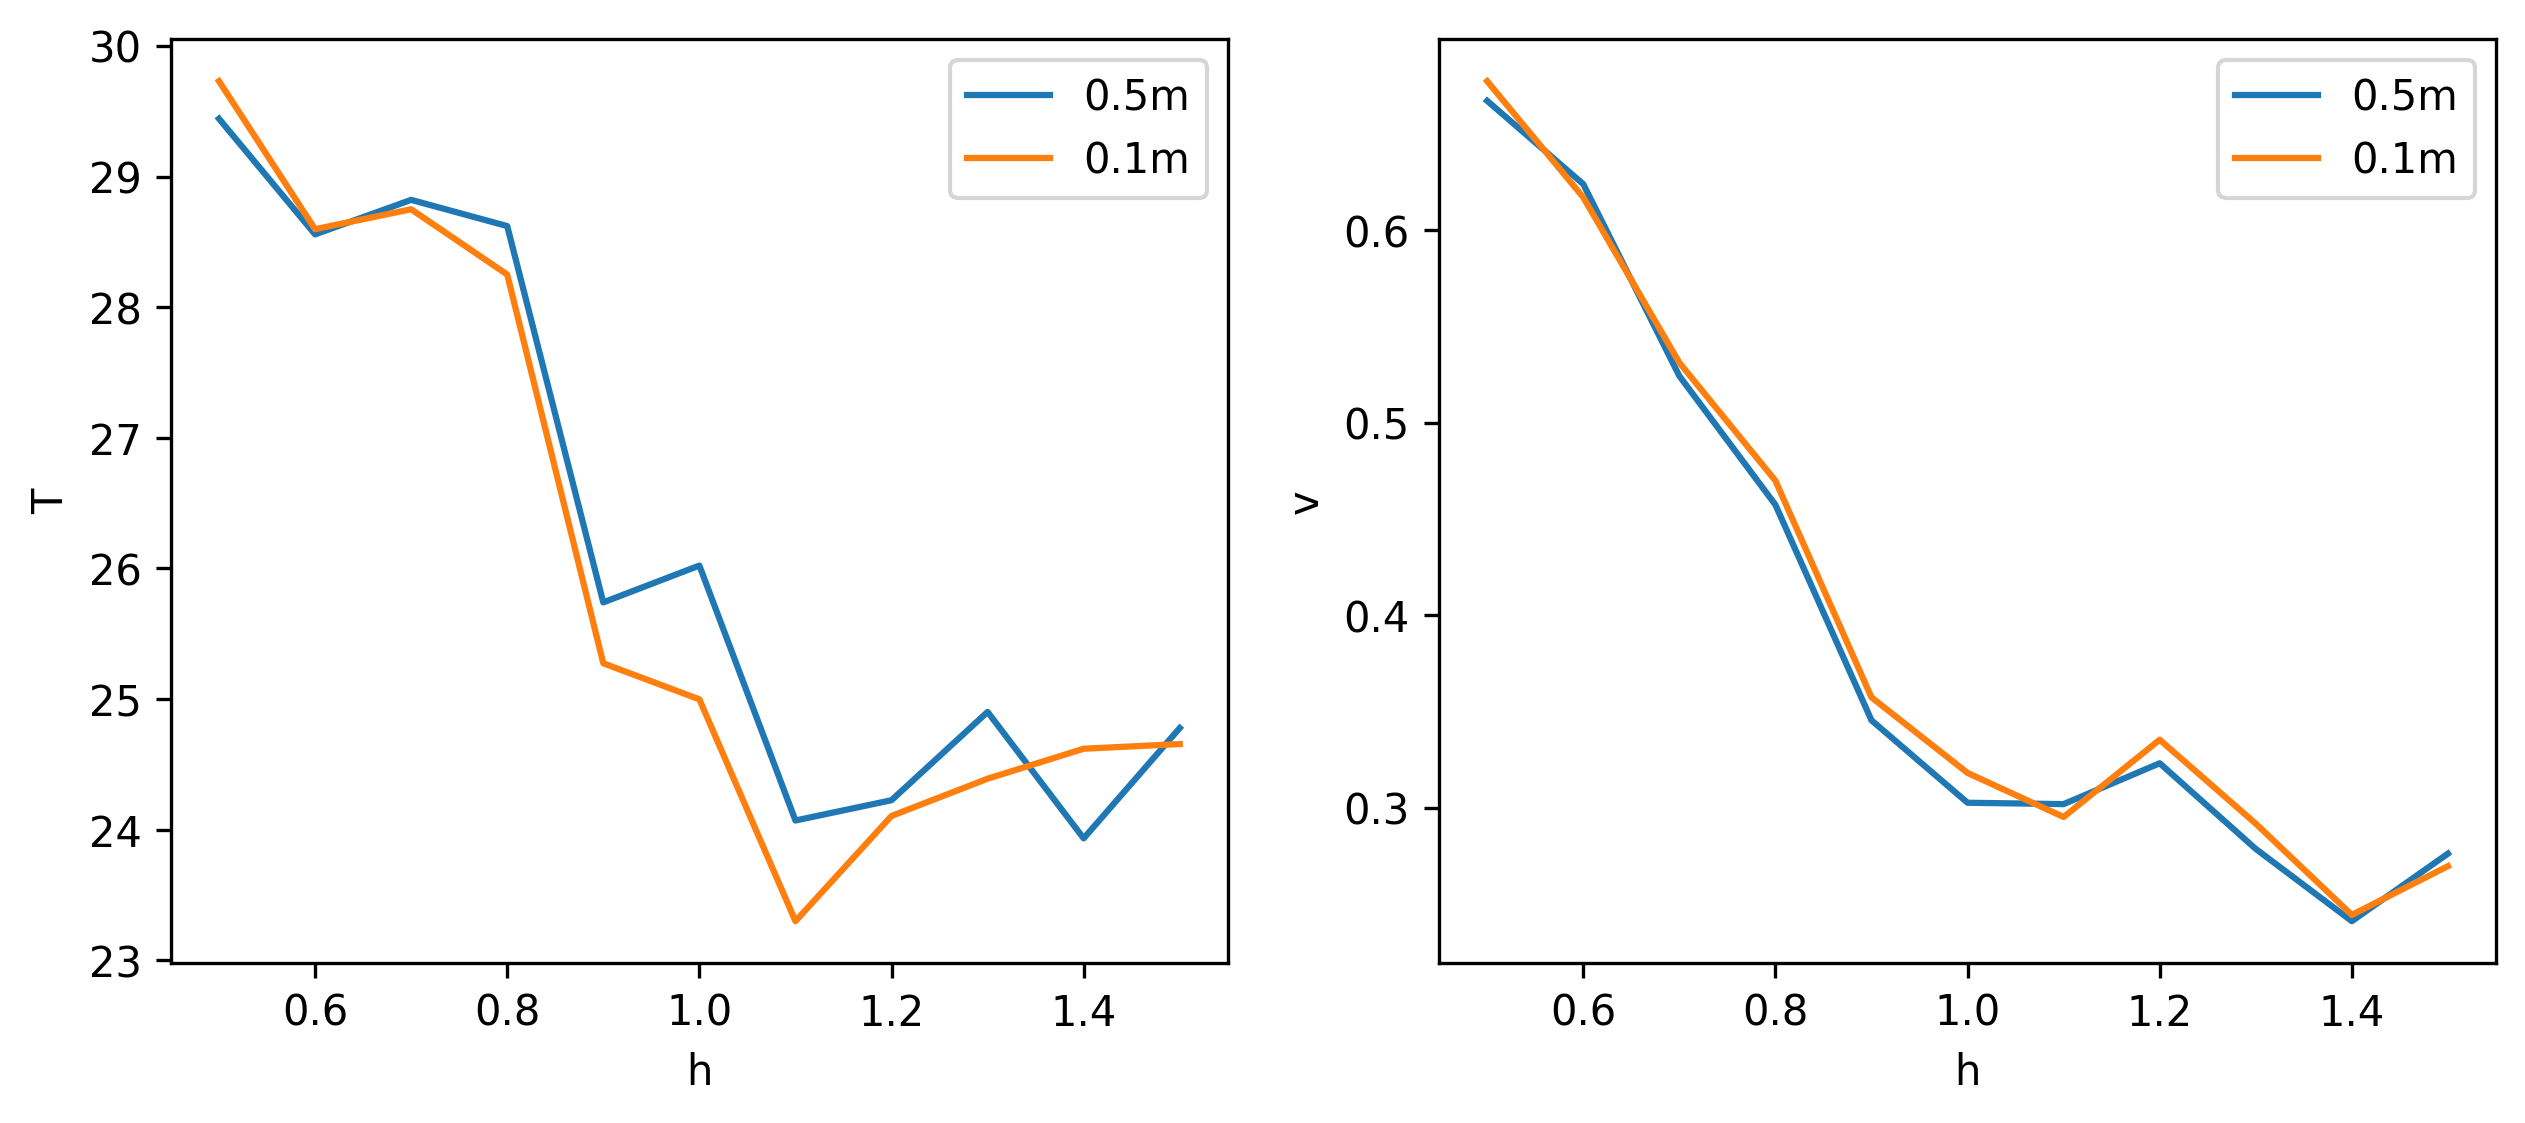
\includegraphics[width=15cm,height=7cm]{figures/H.png}
	\caption{Fan Placement and Temperature-Wind Speed Chart} % 风扇位置与温度风速图
	\label{Fan Placement and Temperature-Wind Speed Chart} % 风扇位置与温度风速图
 \end{figure}

 
Indeed, with the optimization plan we've outlined, not only can it facilitate crop growth, but it also contributes to cost savings. This, in turn, aids in increasing food production.
% 根据我们所给出的优化方案,可以有助于作物生长,同时节省成本开支,这样有助于粮食增产


%%%%%%%%%%%%结论%%%%%%%%%%%%%%%%%%%%%%%%%%
\section{Conclusions}

\subsection{Conclusions of the problem}
\begin{itemize}
\item The research has shown that greenhouse crop productivity is significantly influenced by factors such as temperature, humidity, and wind speed. Our models, which incorporate fluid dynamics, the Navier-Stokes equations, energy conservation, and Darcy-Forchheimer equations, have helped us understand how these factors affect airflow and temperature distribution within the greenhouse.

\item The introduction of the Reynolds number allowed us to simplify the model and study incompressible laminar flow and heat exchange. This revealed insights into how airflow and temperature vary in different greenhouse areas.

\item We also found that crop resistance to fluid flow, as modeled using the Darcy-Forchheimer equation, plays a crucial role in determining the suitability of wind speeds for optimal plant growth. Despite suitable temperatures, suboptimal wind speeds can hinder crop growth.

\item Through simulations, we explored scenarios with different ventilation setups. These simulations indicated that altering the position of vents and adjusting ventilation rates can create more conducive environments for plant growth by optimizing temperature and wind speeds.
\end{itemize}

\subsection{Methods used in our models}
\begin{itemize}
\item Our models employed a combination of fluid dynamics principles, including the Navier-Stokes equations, energy conservation, and the Darcy-Forchheimer equation, to quantify airflow and temperature distribution within greenhouses.

\item We used the Reynolds number to simplify the model and study incompressible laminar flow and heat exchange under greenhouse conditions.

\item The Darcy-Forchheimer equation was incorporated to account for crop resistance to fluid flow, providing a more realistic representation of plant-crop interactions within the greenhouse.

\item Simulations were performed using COMSOL software, allowing us to visualize and analyze the impact of various factors on greenhouse conditions.
\end{itemize}

\subsection{Applications of our models}
\begin{itemize}
\item Our models have practical applications in the optimization of greenhouse environments for crop growth. By understanding how temperature, humidity, and wind speed interact within the greenhouse, we can make informed decisions to enhance crop productivity.

\item These models can aid greenhouse designers and growers in making decisions about vent placement, ventilation rates, and other factors to create optimal conditions for different crops.

\item The insights gained from our research can contribute to the development of more efficient and sustainable greenhouse practices, potentially increasing agricultural yields and reducing resource consumption.
\end{itemize}

%%%%%%%%%%%%未来工作%%%%%%%%%%%%%%%%%%%%%%%%%%
\section{Future Work}
\subsection{Strength and Weakness}

\begin{description}
\item[Strength:] Our models provide a comprehensive framework for understanding and optimizing greenhouse environments. They consider both fluid dynamics and plant-crop interactions, offering a holistic approach to greenhouse management.

\item[Weakness:] One limitation of our models is that they rely on certain assumptions, such as incompressible laminar flow and simplified crop resistance. Future work could focus on refining these assumptions to improve the accuracy of the models.
\end{description}

\subsection{Another model}
\subsubsection{The limitations of queuing theory}
In future research, it would be beneficial to explore the limitations of queuing theory as applied to greenhouse environments. Queuing theory may have its own set of assumptions and constraints that need to be considered in the context of greenhouse crop production.

\subsubsection{More comprehensive parameter consideration}
To further enhance our models, we should consider a more comprehensive range of parameters that influence greenhouse conditions. This could include factors like greenhouse structure, shading, and different plant species. By expanding the scope of parameters, we can develop more robust and adaptable models for greenhouse management.


%参考文献
\begin{thebibliography}{9}%宽度9
\bibitem{1}  Singh M C, Singh J P, Pandey S K, et al. Factors affecting the performance of greenhouse cucumber cultivation-a review[J]. International Journal of Current Microbiology and Applied Sciences, 2017, 6(10): 2304-2323.
\bibitem{2} Liu Y, Li D, Wan S, et al. A long short‐term memory‐based model for greenhouse climate prediction[J]. International Journal of Intelligent Systems, 2022, 37(1): 135-151.
\bibitem{3} Norton T, Sun D W, Grant J, et al. Applications of computational fluid dynamics (CFD) in the modelling and design of ventilation systems in the agricultural industry: A review[J]. Bioresource technology, 2007, 98(12): 2386-2414.
\bibitem{4} Fatnassi H, Boulard T, Poncet C, et al. Optimisation of greenhouse insect screening with computational fluid dynamics[J]. Biosystems Engineering, 2006, 93(3): 301-312.
\bibitem{5} 李万平编. 计算流体力学[M]. 武汉:华中科技大学出版社, 2004.10.
\bibitem{6} 张艺萌.基于CFD的寒地水稻育秧大棚环境数值模拟分析与研究[D].黑龙江八一农垦大学,2018.
\end{thebibliography}


\newpage
%附录

\section{Appendix}
Based on the established mathematical model, this paper uses COMSOL software to perform simulations, and there are no code attachments.
\subsection{Solution to problem 1} % 问题1的求解
\begin{figure}[htbp]
    \centering
    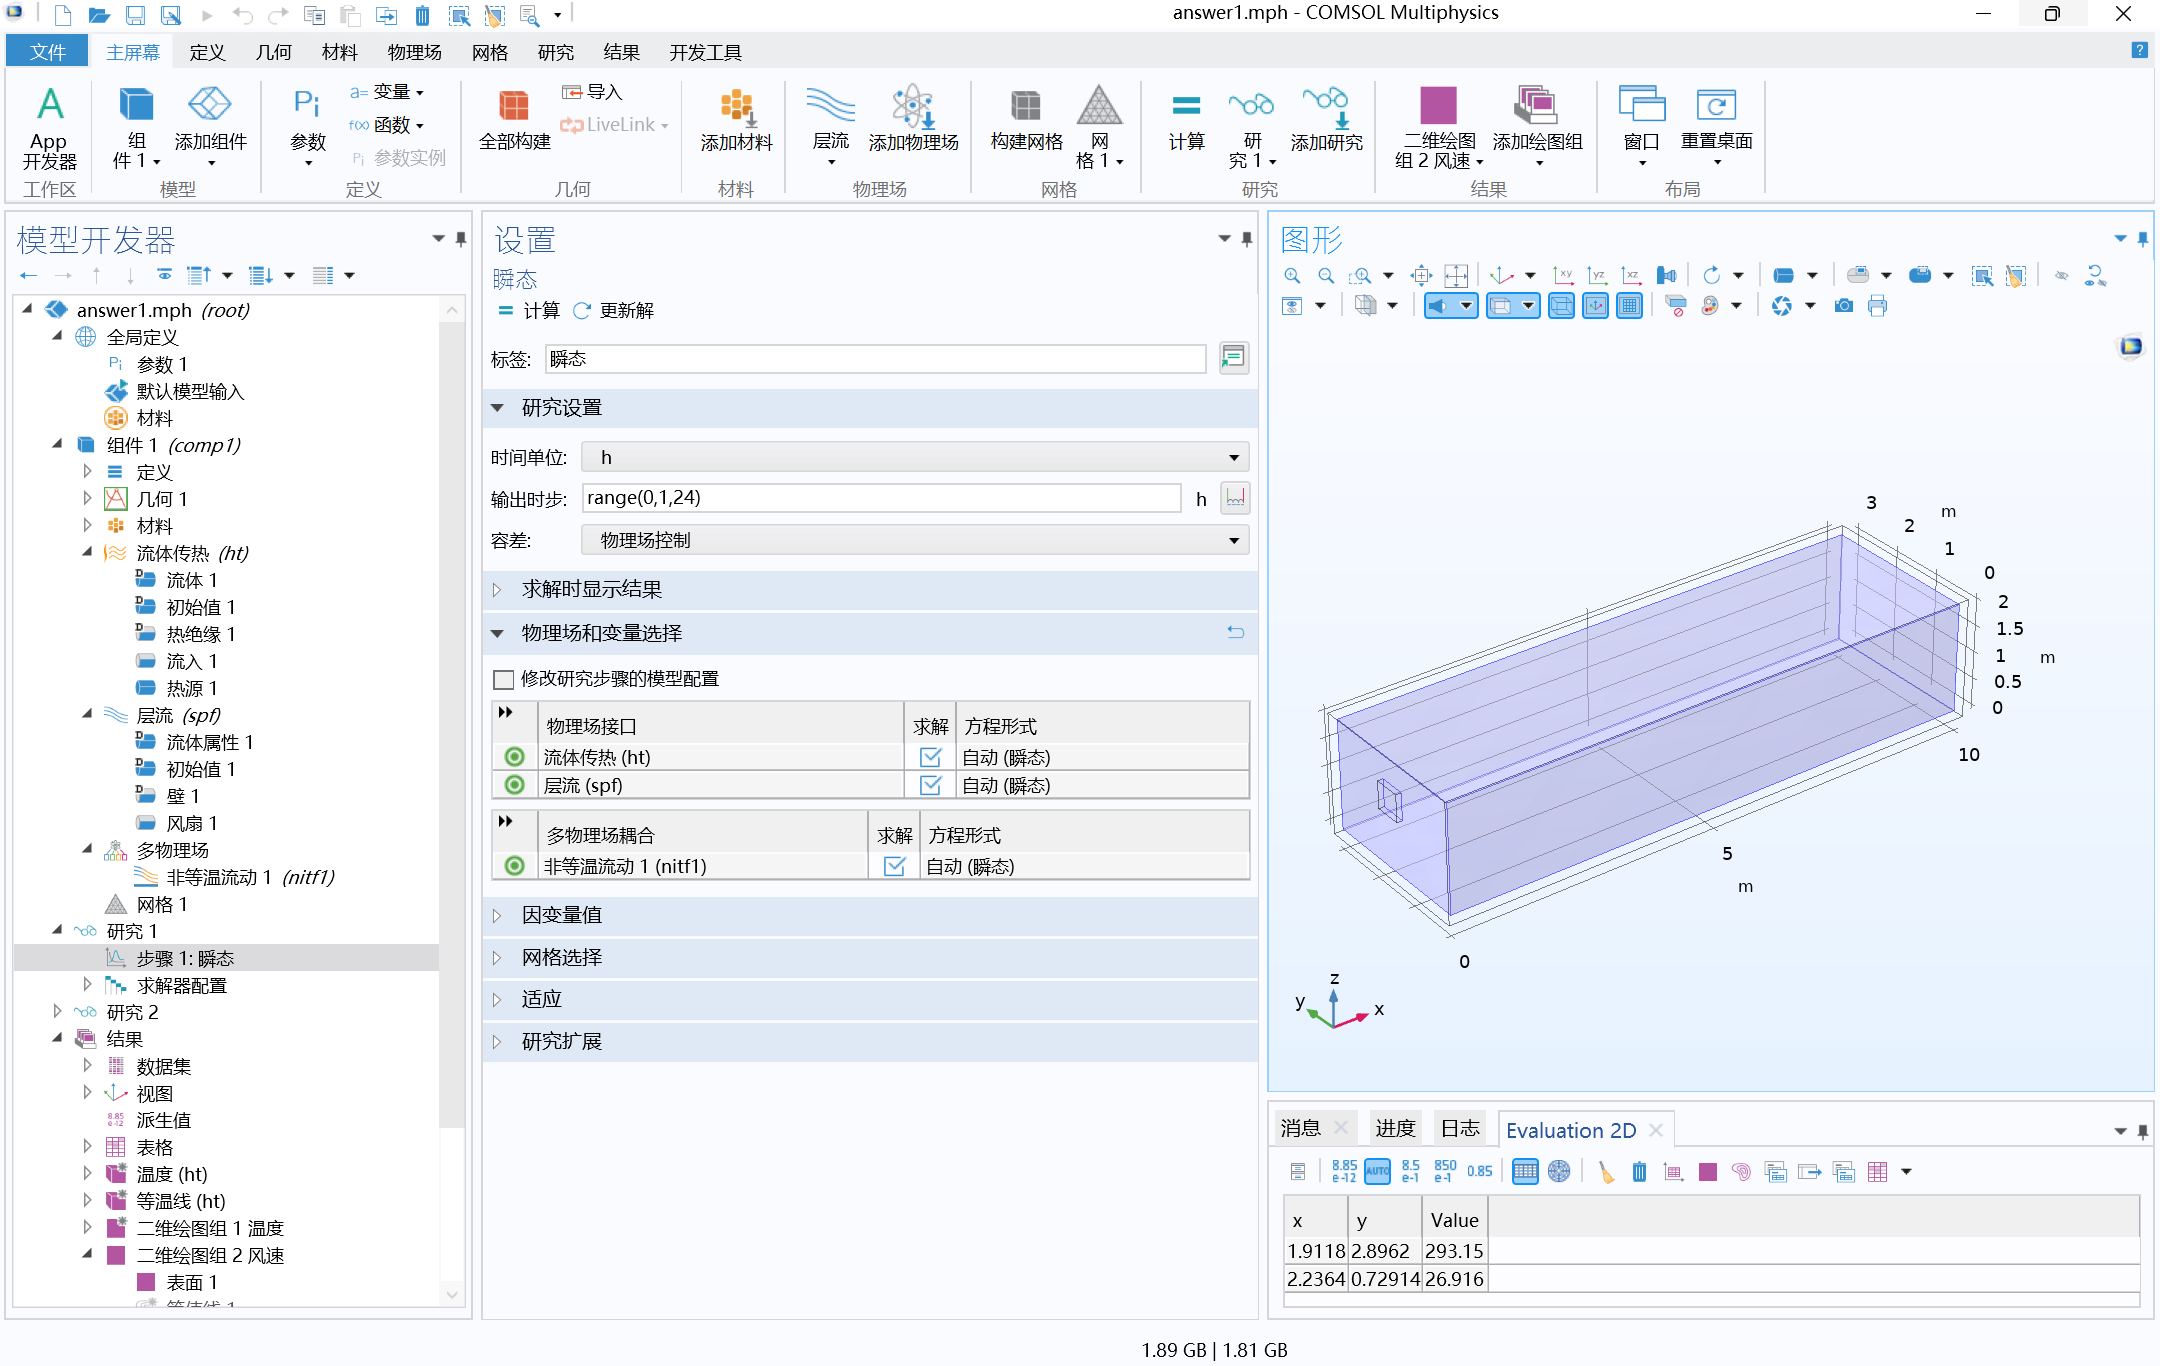
\includegraphics[width=15cm,height=10cm]{figures/last1.png}
\end{figure}
\newpage
\subsection{Solution to problem 2} % 问题1的求解
\begin{figure}[htbp]
    \centering
    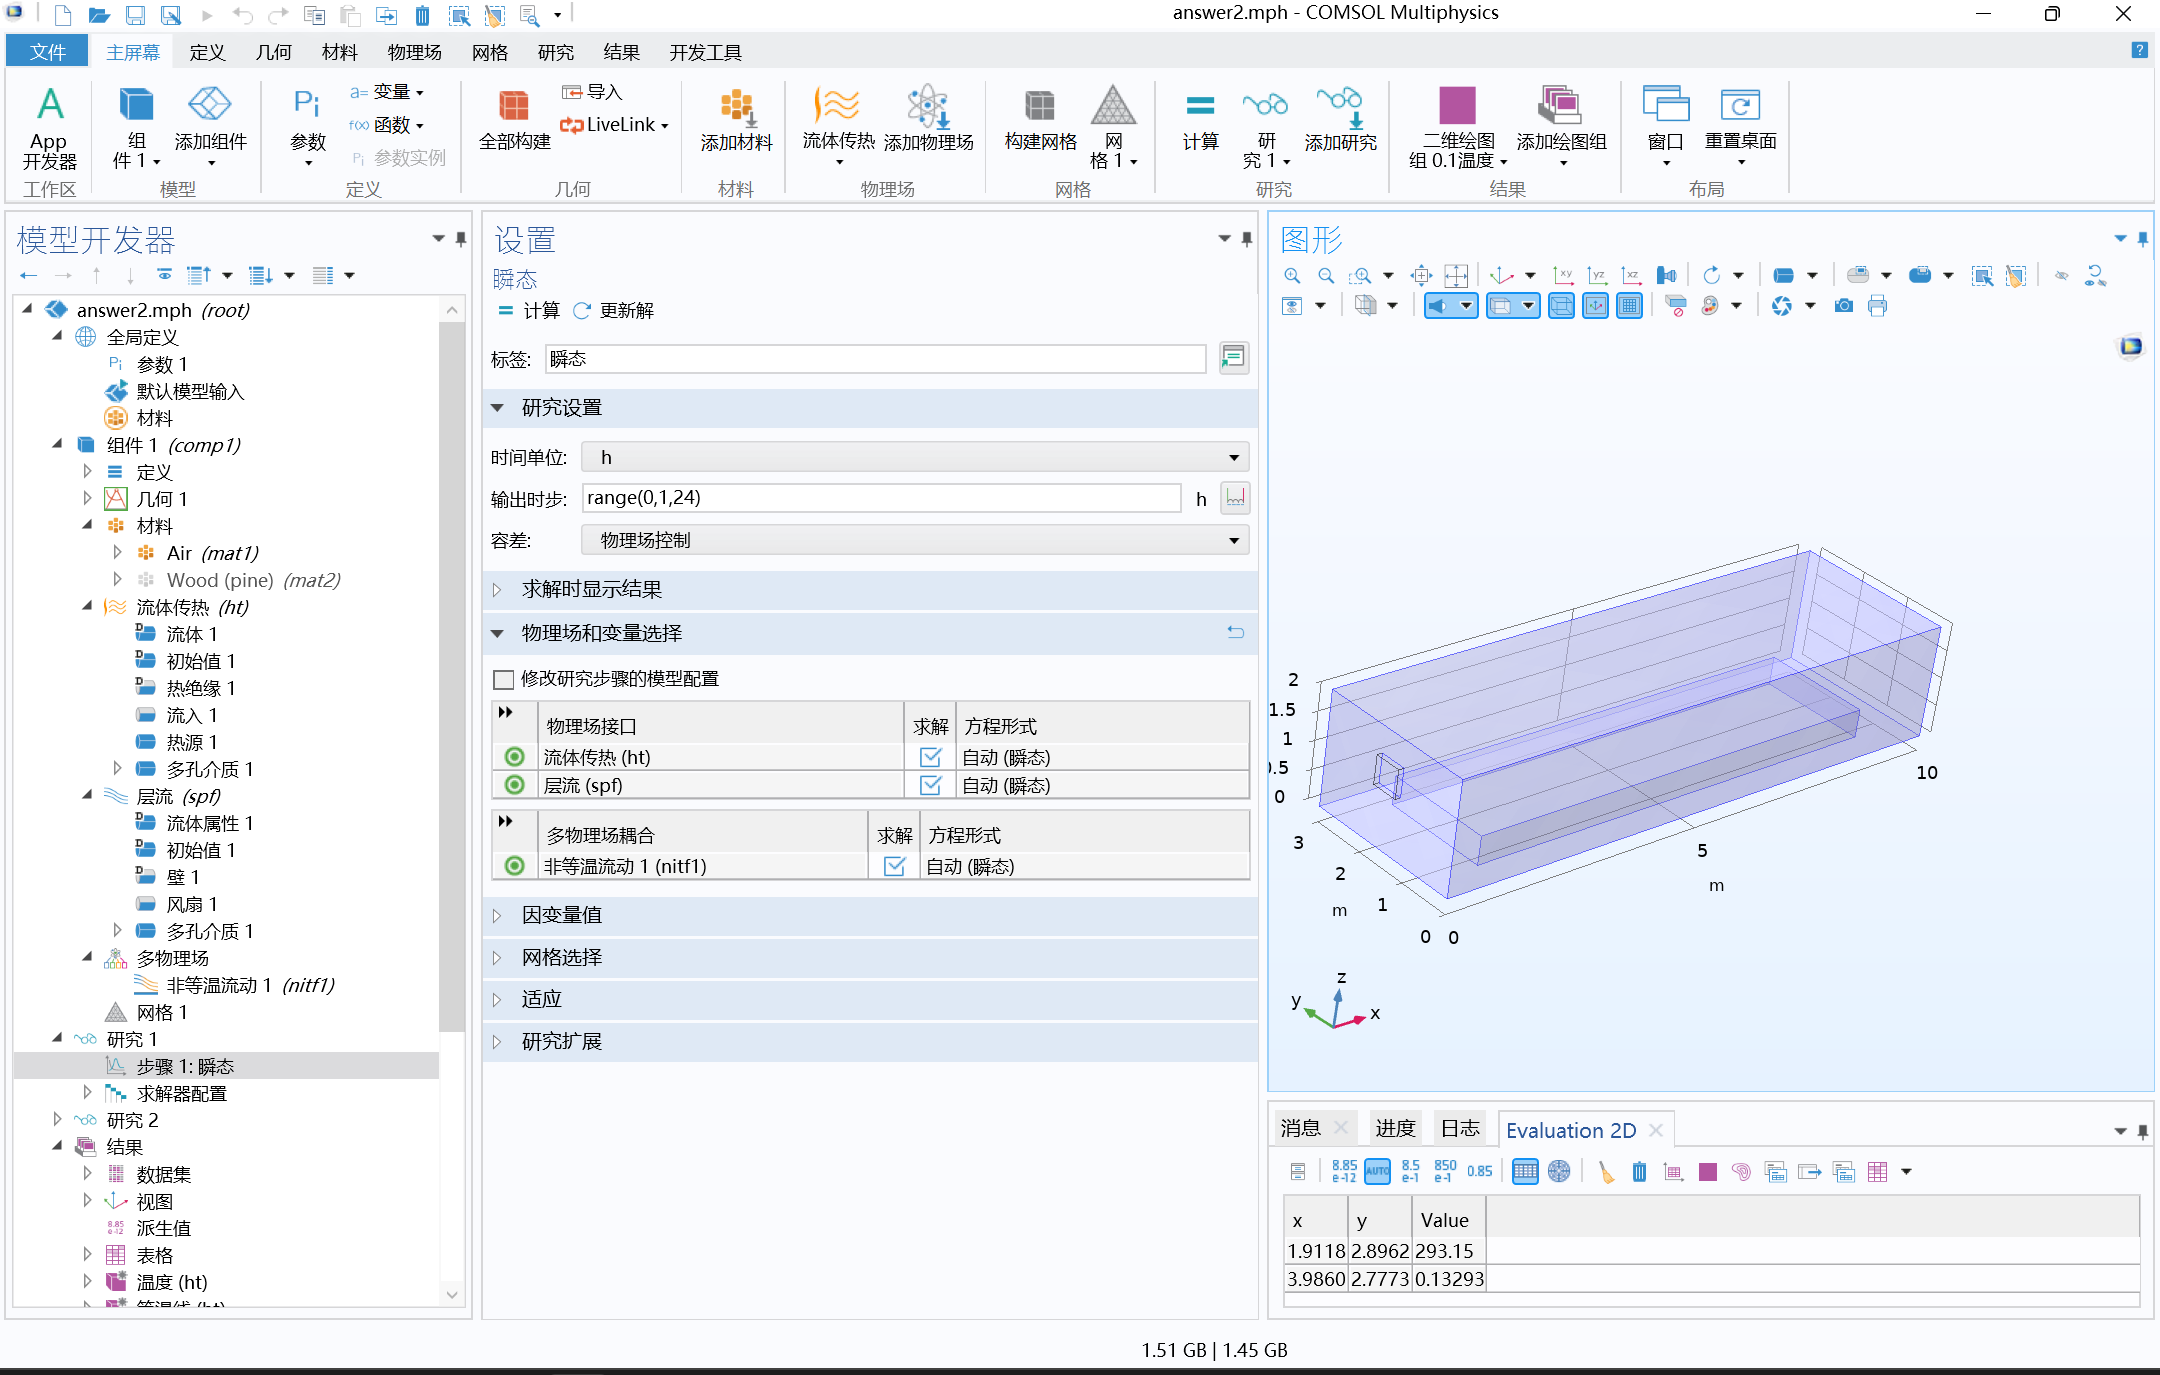
\includegraphics[width=15cm,height=10cm]{figures/last2.png}
\end{figure}

\subsection{Solution to problem 3, 4} % 问题1的求解
\begin{figure}[htbp]
    \centering
    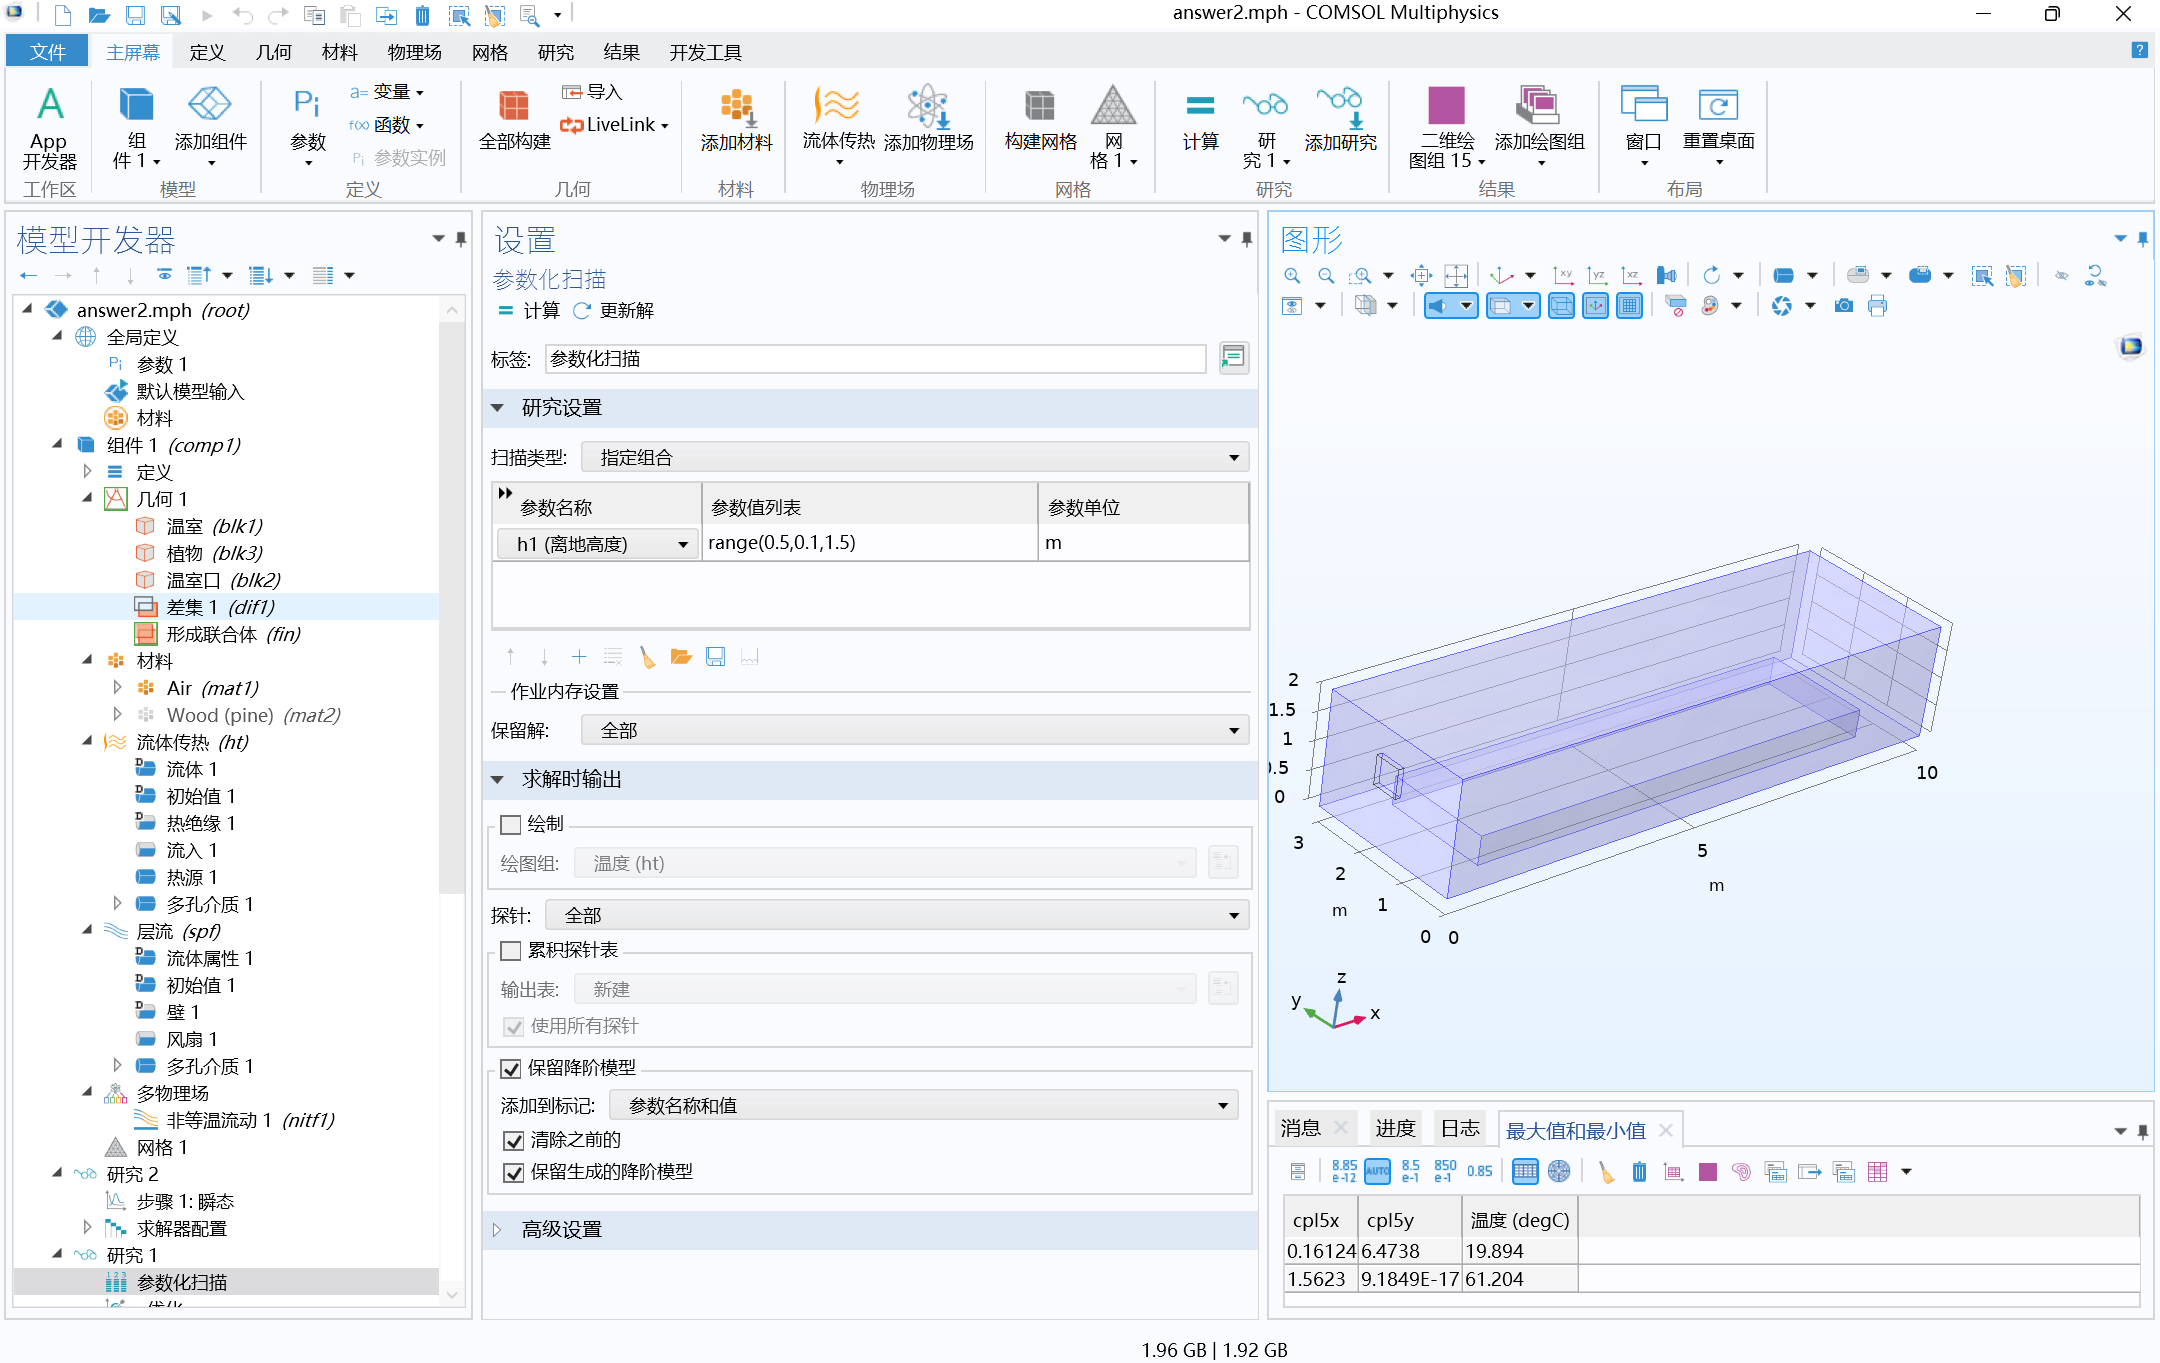
\includegraphics[width=15cm,height=10cm]{figures/last3.png}
\end{figure}
\end{document} 